\documentclass[12pt]{report}
\usepackage[utf8]{inputenc}

% Change font
\renewcommand*\rmdefault{ppl}

% Set margins
\usepackage[margin=35mm]{geometry}

% Equations
\usepackage{mathtools}

% Greek text characters
\usepackage{textgreek}

% Gap between paragraphs
\usepackage{parskip}

% Line spacing
\usepackage{setspace}

% URL formatting
\usepackage{hyperref}

% Algorithm formatting
\usepackage{algpseudocode, algorithm}

% Sideways tables
\usepackage{rotating}

% Table cell colouring
\usepackage{colortbl}

% Ticks and crosses
\usepackage{amsfonts}

% Captions over page
\usepackage{ccaption}

% References in table of contents
\usepackage[nottoc,notlof,notlot,numbib]{tocbibind}

% Page break after sections
\let\oldsection\section
\renewcommand\section{\clearpage\oldsection}

% Monospaced code blocks
\usepackage{listings}
\usepackage{color}
\definecolor{backcolour}{rgb}{0.95,0.95,0.92}
\lstdefinestyle{lststyle}{
    basicstyle=\scriptsize,
    backgroundcolor=\color{backcolour},
}
\lstset{style=lststyle}

\title{In-silico guided prediction of allosteric sites on proteins: application to cyclin-dependent kinase 2}
\author{Joe G Greener}
\date{}

\begin{document}

\maketitle

\onehalfspacing

\begin{abstract}
\thispagestyle{plain}
\setcounter{page}{3}

% Change
Allostery is the functional change at one site on a protein caused by a change at a distant site.
In order for the the benefits of allostery to be taken advantage of, both for basic understanding of proteins and to develop new classes of drugs, the structure-based prediction of allosteric binding sites, modulators and communication pathways is necessary.
Here we review the recently-emerging field of allosteric prediction, focusing mainly on computational methods.
We also describe the search for cryptic binding pockets and attempts to design allostery into proteins.
The development and adoption of such methods is essential or the long-preached potential of allostery will remain elusive.

\end{abstract}


\chapter*{Acknowledgements}


\tableofcontents

\listoffigures

\listoftables

\chapter{Introduction}
\label{cha:introduction}

This chapter introduces the concepts of allostery in proteins, structure-based allosteric prediction, normal mode analysis, the protein structural ensemble, protein kinases and cyclin-dependent kinase 2 (CDK2).
% Change this to fit flow
Some of this introduction has been written as a review (cite).


\section{Allostery in proteins}
\label{sec:introduction_allostery}

Allostery in its broadest sense is the functional change at one site on a protein caused by a change at a distant site.
The perturbation at the allosteric site can be non-covalent binding of a molecule (e.g.\ small molecule, ions, RNA, DNA), covalent binding (e.g.\ phosphorylation) or light absorption \cite{Nussinov2013}.
Changes in structure or dynamics lead to effects such as a reduction or increase in catalytic activity, changes in disordered regions or changes in oligomerisation state.

% Add MWC/KNF/Perutz/Hilser2012/Tsai2014 refs back
% And Csermely for networks
% Panjkovich2010
% All protein potentially allosteric Gunasekaran2004
Since the first discovery of allosteric systems more than 50 years ago there have been various models put forward to describe the phenomenon.
The dominant proposals for many years were the Monod-Wyman-Changeux (MWC) model, which posited that pre-existing states are subject to an equilibrium shift on modulator binding, and the Koshland-N\'{e}methy-Filmer (KNF) model, which advanced the idea that there was an induced fit of a binding site on interaction with a modulator \cite{Motlagh2014}.
The structural view of allostery, which aimed to elucidate the allosteric mechanism by finding structural changes on effector binding, began to fill the gaps left by the phenomenological MWC and KNF descriptions.
The discovery that entropic contributions to allostery can be significant predicted the phenomenon of allostery without conformational change \cite{Cooper1984}, where the allosteric effect is communicated by a change in protein dynamics rather than protein structure \cite{Motlagh2014}.

More recently these views on allostery have been revisited and reconciled in approaches that focus on the ensemble of conformational states that proteins exist in \cite{Motlagh2014, Cui2008}.
Figure~\ref{fig:allostery} outlines the current understanding of allostery.
A perturbation at any site in the structure leads to a shift in the occupancy of states by the population, so allostery is a property of the conformational ensemble.
The effect at the allosteric site is linked to the active site by small conformational changes that transmit the allosteric effect in a wave-like manner along pathways of amino acids in the protein \cite{DelSol2009}.
These pathways may be conserved by evolution.
It is also important to consider the effect of allostery on cellular networks and reaction pathways \cite{Nussinov2013}, with allosteric effects propagating via protein-protein interactions.

Allosteric drugs have hardly been explored and hold many potential benefits over orthosteric (non-allosteric) drugs: they are highly specific as they do not bind to active sites that are often conserved in protein families; they can activate as well as inhibit a protein; and they can have a ceiling to their effect \cite{Wenthur2014}.
Allosteric modulators have been elucidated for targets as diverse as G protein-coupled receptors (GPCRs), protein kinases, the GABA receptor, hepatitis C virus polymerase and RNA.
Numerous other allosteric modulators are in various stages of human clinical trails.
However, discovery of allosteric drugs presents challenges beyond those encountered in orthosteric drug discovery - see later.

In order to understand and utilise allostery it is necessary to be able to predict allosteric sites, allosteric modulators and residues involved in propagating the allosteric signal.
This review outlines advances from the last few years in the structure-based prediction of protein allostery, largely focusing on computational approaches.
Previous reviews have covered similar topics \cite{SchuelerFurman2016, Wagner2016, Guarnera2016, Lu2014}.
The emerging fields of cryptic allosteric site discovery and allosteric site design are described.

% Other stuff from Nussinov
% https://www.nature.com/articles/ncomms16018.pdf - The self-inhibitory nature of metabolic networks and its alleviation through compartmentalization - mention at network point?


\begin{figure}
\centering

\includegraphics[width=0.9\textwidth]{figures/allostery/allostery}
% Touch up and ensure symmetry

\caption[The current conception of allostery as a property of the conformational ensemble]
{The current conception of allostery.
(A) A two-state model of allostery where a protein has an active and an inactive conformation.
In the presence of the allosteric inhibitor the inactive state is favoured either by the inhibitor binding to the protein when it is in the inactive state (red arrow - conformational selection) or by the inhibitor binding to the active state and causing inactivation (blue arrow - induced fit).
(B) The variety of motions that can lead to allostery.
Larger motions or more disorder are shown further down the vertical axis.
Figure based on Figure~2 from \cite{Motlagh2014}.
(C) A simplified representation of the change in the energy landscape on binding of an allosteric inhibitor.
The shaded regions show the main occupied conformation in each case.
On inhibitor binding the relative energies of the active and inactive states are altered.
For example, disruption of a hydrogen bond could destabilise the active state and stabilise the inactive state.
(D) Glucokinase, a well-studied example of allostery \cite{Kamata2004}, is shown as a yellow cartoon.
The glucose substrate and the allosteric modulator are shown as spheres coloured by element.
The active site and allosteric site are coloured purple and green respectively.}

\label{fig:allostery}
\end{figure}


\subsection{Computational methods for allosteric prediction}

The last few years have seen the emergence of the first general methods that predict allostery based on protein structure.
Table~\ref{tab:allosteric_methods} summarises these methods, many of which are available as web servers.


\begin{sidewaystable}
\centering

\begin{footnotesize}
\begin{tabular}{ l l p{5cm} l l }
\hline
Name & Reference(s) & Output(s) & Web server available & Source code available online \\
\hline
AlloPred & \cite{Greener2015} & Predicted allosteric pockets & \url{http://www.sbg.bio.ic.ac.uk/allopred/home} & Yes, MIT licence \\
AlloSigMA & \cite{Guarnera2017} & Allosteric free energies & \url{http://allosigma.bii.a-star.edu.sg/home} & No \\
AlloSite & \cite{Huang2013} & Predicted allosteric pockets & \url{http://mdl.shsmu.edu.cn/AST} & No \\ % AlloSitePro?
AllosMod & \cite{Weinkam2012} & Modelled energy landscapes & \url{http://modbase.compbio.ucsf.edu/allosmod} & No \\
% Bond propensity method & \cite{Amor2016} & Residues coupled to active site & No & No \\
ENM method & \cite{Li2017} & Residues coupled to normal modes & \url{http://enm.pitt.edu} & Partly as ProDy, MIT licence \\
ExProSE & \cite{Greener2017} & Ensemble of protein structures,\newline predicted allosteric pockets & No & Yes, MIT licence \\
MCPath & \cite{Kaya2013} & Allosteric communication pathways & \url{http://safir.prc.boun.edu.tr/clbet_server} & No \\
% MixMD & \cite{Ghanakota2016} & Fragment-binding allosteric hotspots & No & No \\
PARS & \cite{Panjkovich2014, Panjkovich2012} & Predicted allosteric pockets & \url{http://bioinf.uab.cat/pars} & No \\
SPACER & \cite{Goncearenco2013, Mitternacht2011} & Predicted allosteric residues,\newline exploration of allosteric communication & \url{http://allostery.bii.a-star.edu.sg} & No \\ % Or predicted allosteric sites?
STRESS & \cite{Clarke2016} & Predicted surface-critical and interior-critical residues & No & Yes \\ % Server was http://stress.molmovdb.org but down
\hline
\end{tabular}
\end{footnotesize}

\caption[Computational allosteric prediction methods currently available to run locally or as a web server]
{Computational allosteric prediction methods currently available to run locally or as a web server, ordered alphabetically.
In addition there are various pocket prediction methods that aim to predict binding pockets on proteins, but not specifically allosteric pockets \cite{Huang2006, LeGuilloux2009, Cimermancic2016}.}

\label{tab:allosteric_methods}
\end{sidewaystable}


\subsubsection{Normal mode analysis}

In normal mode analysis (NMA) the structural fluctuations of a protein around an equilibrium conformation are decomposed into harmonic orthogonal modes \cite{Hayward2008}.
The process of NMA is shown in Figure~\ref{fig:nma}.
Each mode has all parts of the system moving sinusoidally, in phase and with the same frequency.
All observed configurations of the system can be generated from a linear combination of its normal modes.
The normal modes are found by diagonalising the Hessian matrix - the matrix of second derivatives of the potential energy with respect to the mass-weighted atomic coordinates.
% Have equations here?
NMA is effective at describing protein dynamics, despite ignoring the complex nature of the protein energy landscape \cite{Bahar2005}.
Even considering the C\textsuperscript{\textalpha} atoms alone as a network of balls and springs can be sufficient, meaning NMA is a computationally efficient way of exploring protein flexibility compared to MD.
The long-range nature of allosteric communication is often well-described by low-frequency modes that involve the motion of many atoms.
However, allostery does involve local effects so higher-frequency modes should also be taken into account \cite{Collier2013}.
The long-range nature of allosteric communication is often well-described by low-frequency modes that involve the motion of many atoms.
The binding leverage approach \cite{Mitternacht2011} predicts how ligand binding couples to the intrinsic motions of a protein.
Sites with high binding leverage are predicted to be allosteric.
Binding leverage was developed into the web server SPACER \cite{Goncearenco2013}, and into the general predictor STRESS \cite{Clarke2016} by a different group.
% Mention other Mitternacht methods? Geometry/local closeness
% This has been further developed \cite{Guarnera2016a}...
% And turned into a web server \cite{Guarnera2017}...
The PARS method \cite{Panjkovich2012, Panjkovich2014} calculates normal modes in the presence and absence of a simulated allosteric modulator.
If the motions are significantly different the site is predicted as allosteric.
The AlloPred method \cite{Greener2015} calculates the normal modes of a protein, then holds the springs in the region of a potential allosteric site rigid and measures the effect of this perturbation at the active site.
The DynOmics ENM server \cite{Li2017} finds hinge residues that control the two slowest normal modes of a protein, and hence are able to influence its dynamics.
Several studies have used NMA to model allosteric regulation in specific sets of proteins \cite{Balabin2009, Rodgers2013, Zheng2007}.
NMA is suitable for high-throughput, automated approaches as it can be computationally inexpensive.
However whilst NMA-based methods might be expected to reveal perturbations to vibrations, the assumption of harmonic fluctuations around an energetically-minimum structure means that other contributing motions to allostery such as local unfolding and rigid body movements \cite{Motlagh2014} are not taken into account.
% \cite{Su2014}? probably not
% Add Taguchi 2016
% Other bits from Hayward2008
% Say equations in AlloPred methods


\begin{figure}
\centering

\includegraphics[width=\textwidth]{figures/nma/nma}

\caption[Steps in normal mode analysis]
{Steps in NMA.
A protein structure is converted into an elastic network where balls are C\textsuperscript{\textalpha} atoms and springs are between C\textsuperscript{\textalpha} atoms within a certain distance.
A Hessian matrix of second derivatives of the potential energy $V$ in terms of the mass-weighted atomic coordinates $q_{i}$ is derived from the potential energy function of this elastic network.
Diagonalising the Hessian matrix yields eigenvectors and eigenvalues that correspond to the displacements for each C\textsuperscript{\textalpha} atom in the mode and the square of the mode frequency respectively.
See \cite{Hayward2008} for more.}

\label{fig:nma}
\end{figure}


\subsubsection{Machine learning}

A few methods have used machine learning to predict allostery.
AlloSite \cite{Huang2013} uses a support vector machine and features from Fpocket \cite{LeGuilloux2009} to re-rank pockets in terms of their allosteric character.
However the results are often found to be similar to the Fpocket ranking, showing the difficulty of distinguishing pockets that have specific allosteric character from those that are generally suitable for ligand binding.
% AlloSitePro? Song2017
A Random Forest approach \cite{Chen2016} uses descriptors for binding sites and associated ligands to assign protein cavities as allosteric, regular or orthosteric.


\subsubsection{Molecular dynamics}

Molecular dynamics (MD) remains the standard computational tool for structural analysis when structures are available.
A study on the signaling protein NtrC combined MD simulations and NMR data to explore the free energy landscape and investigate at atomic resolution the transition from active to inactive state \cite{Pontiggia2015}.
% Add \cite{Qi2012} here
% And Laine2010
Perturbation response scanning (PRS), in which the response of the structure to random perturbations at specific positions is examined, is a popular tool for allosteric prediction.
% Cite here others cited elsewhere in the paper that use PRS?
For example, allosteric hotspot residues were predicted using PRS for the chaperone Hsp70 \cite{Penkler2017}.
Weinkam et al.\ constructed energy landscapes and explored them with MD \cite{Weinkam2012}.
They were able to study the allosteric mechanisms involved in three proteins.
The method is available as the AllosMod web server.


\subsubsection{Evolutionary methods}

Classic work has shown that allosteric communication can be mediated by networks of residues conserved by evolution \cite{Lockless1999, Suel2003}.
One study developed previous work on protein sectors, groups of co-evolving residues physically contiguous in structure, to link sector-connected surface sites to allosteric sites \cite{Reynolds2011}.
A recent approach found that surface and interior critical residues tend to be conserved \cite{Clarke2016}.
The recent discovery that most directly co-evolving residues distant in 3D structure are close in related structures or assemblies \cite{Anishchenko2017} brings into question the concept of allosteric and active sites that directly co-evolve.
As more structural and conservation information is acquired it will be important to discover to what degree allostery in proteins is a result of selection on specific pathways, and to what degree novel allostery can be discovered on proteins in the absence of previous evolutionary pressure.
% Be clear difference between conservation and co-evolution


\subsubsection{Other methods}

A recent study \cite{Amor2016} constructs an all-atom graph and calculates for each bond the bond propensity, the strength of coupling to the active site through the graph.
The method is used to reproduce observed results for three proteins in detail and is also able to predict allosteric sites in a dataset of 20 allosteric proteins.
ExProSE \cite{Greener2017} takes two structures of the same protein and generates an ensemble of structures using distance constraints.
By adding extra constraints at a possible allosteric site, a perturbed ensemble is generated.
By comparing ensembles with and without the allosteric perturbation, allosteric sites can be predicted and the effect of perturbation on structure and dynamics can be explored.
This work also includes a quantitative comparison of available allosteric site prediction methods.


\subsubsection{Methods not specific to allostery}

The identification of binding sites on the protein surface is a problem that has long pre-dated the search for pockets that are specifically allosteric.
These methods are however useful in the structure-based prediction of allostery - the identification of a high-affinity binding site distant from a known active site could present an opportunity for allosteric regulation, for example.
The FTMap family of web servers \cite{Kozakov2015} predicts ligand-binding hotspots using small organic molecules as probes on the protein surface.
By using mixed-solvent MD this principle has been extended to the prediction of allosteric sites in particular, with success on some test cases \cite{Ghanakota2016}.
Common pocket prediction methods such as LIGSITE\textsuperscript{\it csc} \cite{Huang2006} and Fpocket \cite{LeGuilloux2009} are able to find pockets on a protein large enough to bind small molecules, and these often correspond to allosteric sites \cite{Greener2017}.


\subsubsection{Allosteric pathway prediction}

% Add Kidd2009
Allosteric signals can be propagated by multiple communication pathways \cite{DelSol2009}.
Understanding these pathways is necessary in order to predict sites that are able to communicate with the active site \cite{Dokholyan2016}.
A machine learning approach to predict residues involved in allosteric communication uses a variety of structural and network features and is able to predict these hotspots with reasonable accuracy \cite{Demerdash2009}.
A different approach, McPath, uses a Monte Carlo algorithm to define likely allosteric pathways by examining inter-residue interactions in a residue network \cite{Kaya2013}.
A study that added an allosteric domain to a protein analysed residue contact maps to find loops mechanically-coupled to the active site \cite{Dagliyan2016}.
An investigation on the PDZ domain using MD found that allosteric changes are non-linear and occur in a non-local fashion, and are similar in many ways to protein folding \cite{Buchenberg2017}.


\subsection{Experimental methods for allosteric prediction}

Experimental studies such as crystallography, NMR and site-directed mutagenesis remain the best tools for exploring allostery in a particular protein.
A synthetic azetidine derivative that kills Mycobacterium tuberculosis through allosteric inhibition of tryptophan synthase (TrpAB), a previously untargeted enzyme, was found by a high-throughput screen \cite{Wellington2017}.
The inhibition is not easily overcome by changes in metabolic environment due to the modulator binding at the TrpAB \textalpha -\textbeta -subunit interface and affecting multiple steps in the overall reaction of the enzyme.
A study on the proteasome \cite{Haselbach2017} crystallised the complex in the presence and absence of an allosteric modulator.
Having the active and inactive structures allowed the authors to propose a detailed mechanism of inactivation, which has implications for future allosteric proteasome inhibitors.
A study on flavovirus protease \cite{Brecher2017} used a virtual screen to select 29 potential allosteric compounds that were tested experimentally.
One showed an ability to inhibit the conformational change and also inhibit flavovirus growth.
Allosteric pathways in ERG proteins were proposed using fluctuation correlation data and validated by mutating residues in the pathways \cite{Ye2017}.
However, there are limits to the use of mutational studies to validate allosteric mechanisms.
It has been found that mutational data can give evidence for a deliberately poorly-conceived allosteric mechanism \cite{Tang2017}.
In the future it is to be hoped that experimental screens specifically for allosteric sites \cite{Martin2012, Jayakar2017, Pellerano2017, Pisco2017, Raman2014} become more widespread, opening the path to conventional large-scale screens for allosteric drugs.
% http://www.jbc.org/content/292/15/6429.full.pdf+html "Allostery modulates the beat rate of a cardiac pacemaker" NMR used
% Dror 2013 "Structural basis for modulation of a G-protein-coupled receptor by allosteric drugs" - actually this could go in MD section with a reference to long MD becoming more feasible
% https://www.nature.com/nsmb/journal/vaop/ncurrent/pdf/nsmb.3440.pdf - An information theoretic framework reveals a tunable allosteric network in group II chaperonins - could go in evolution section
% Shen2017 genomic screen


\subsection{Cryptic allosteric sites}

The discovery of cryptic binding pockets - pockets that are only available in some conformations of the protein and may not have an associated experimental structure - has the potential to vastly increase the number of druggable sites on proteins \cite{Boehr2009} and is directly relevant to allosteric prediction.
A recent study \cite{Lee2016} showed using NMR data that ligands of the LpxC enzyme access a cryptic site that is invisible to crystallography.
One study used Markov state modelling and MD to predict multiple hidden allosteric sites on \textbeta -lactamase and tested these using thiol labelling experiments \cite{Bowman2015}, later finding modulators for the sites \cite{Hart2017}.
The general approach CryptoSite uses machine learning to predict cryptic pockets on proteins using sequence and structural features \cite{Cimermancic2016}.
However, two problems affect the use of cryptic allosteric pockets over allosteric sites where the pocket is present in most or all conformations.
Firstly, the shape of the pocket is not known so rational drug design is difficult.
Secondly, there is potentially an energetic cost associated with the protein adopting the conformation required for the cryptic pocket \cite{Oleinikovas2016}.
However, the discovery of ligands with inhibition constants in the low picomolar range in the above study \cite{Lee2016} show that these sites are druggable.
Further computational and experimental studies are required to explore this promising area.


\subsection{Design of allosteric sites}

The rational design of allosteric sites is a problem closely related to structure-based prediction of allostery.
Introducing allosteric sites into existing proteins, or creating fusion proteins to add activity switches, has many potential applications including in biotechnology \cite{Makhlynets2015}.
A recent study added a PDZ domain into the Cas9 protein at a site that did not disrupt enzyme action \cite{Oakes2016}.
The protein showed modulator-dependent activity in cells, establishing a system for Cas9 activation.
Another study created fusion proteins that use conformational entropy to respond to temperature or pH as a switch \cite{Choi2015}.
Taylor et al.\ engineered \textit{E.\ coli} LacI to respond to one of four new inducer molecules using computational design and mutagenesis \cite{Taylor2016}.
Dagliyan et al.\ designed a protein with a unique topology, uniRapR, whose conformation is controlled by the binding of a small molecule \cite{Dagliyan2013}.
The switching and control ability of uniRapR was confirmed in silico, in vitro, and in vivo.
uniRapR was used as an artificial regulatory domain to control activity of kinases as a proof of concept.
The same group built on this and inserted the light-sensitive LOV2 domain into 3 proteins at non-conserved, surface-exposed loops identified computationally using residue contact analysis as being allosterically coupled to active sites \cite{Dagliyan2016}.


\subsection{Discussion of allostery}

It is challenging to compare different methods for allosteric prediction.
The different inputs and, more commonly, outputs make systematic comparisons difficult.
One quantitative comparison indicated broadly similar performance between four available methods \cite{Greener2017}.
One of the Critical Assessment of Genome Interpretation challenges in 2015-16 focused on predicting the influence of mutations on the allosteric regulation of human liver pyruvate kinase \cite{Xu2017}.
However the uptake was limited to four groups and the predictive ability was marginally better than random.
In the long run a dedicated community-wide initiative similar to the Critical Assessment of Structure Prediction \cite{Moult2016} would be beneficial to the field of allosteric prediction.

One factor holding allosteric prediction back is the lack of a varied and robust set of benchmarks to test methods against.
ASBench \cite{Huang2015} is a curated set of allosteric proteins, and has been used for example to benchmark AlloPred \cite{Greener2015}.
It is a subset of the AlloSteric Database (ASD, \url{http://mdl.shsmu.edu.cn/ASD}) \cite{Shen2016}.
ASD v3.0 contains over 1,400 proteins and also includes allosteric mechanisms, allosteric networks of proteins and `allosteromes' of the allostery involved in protein kinases and GPCRs.
Improvements in such resources are necessary to prevent the developers of new methods having to assemble their own datasets \cite{Panjkovich2012, Mitternacht2011, Amor2016} and to allow systematic comparisons between methods.
% Need more studies like Haselbach2017, Ozorowski2017 that get structure with and without modulator and compare

An issue that requires more study in the field of allosteric prediction is the exact relationship between an allosteric modulator and whether it acts as an activator or inhibitor.
It has been shown that under different conditions the same allosteric modulator can have opposite effects \cite{Motlagh2012}.
Another viewpoint is the anchor/driver model of allostery, with the concept of a pushing or pulling driver determining which way the ligand acts \cite{Nussinov2014}.
An approach to study this would be a quantitative structure activity relation-like study where a variety of modulators and conditions are explored on the same protein.
This would give evidence as to whether small structural differences causing a pushing or pulling effect are enough to reliably switch activator/inhibitor action.

The mechanism of dynamic allostery, where the allosteric effect is transmitted through changes in dynamics and the average structure does not necessarily change, also requires further investigation.
While experimental studies \cite{Popovych2006, Capdevila2017, Wellington2017} have found evidence for dynamic allostery, Nussinov and Tsai \cite{Nussinov2015} warn that an apparent lack of conformational change can be an artefact of various factors such as crystal packing, crystallisation conditions, disorder to order transitions, incremental activation, synergy between allosteric sites and changes in oligomeric state.
A recent MD study proposes that allostery in the well-studied PDZ domain is driven by changes in electrostatic effects rather than solely changes in dynamics \cite{Kumawat2017, Liu2017}.
The role of water in allostery also needs to be further explored as evidence has been found that re-arrangement of water molecules is a possible mechanism of allostery \cite{Buchli2013, Amor2016}.


Challenges faced in the structure-based prediction of protein allostery:

\begin{enumerate}
\item As shown in Figure 1B, an allosteric effect can arise from a variety of different mechanisms.
A general predictor would have to account for these in a unified manner.
This is particularly challenging when disorder is involved, as approaches based on a defined structure are less applicable.
Some approaches to studying disorder and allostery have been proposed \cite{Singh2017, Wang2017}.
\item The conformational changes that cause allostery are often large enough to occur on timescales of microseconds or milliseconds.
This makes them too computationally expensive to study using MD without the use of accelerated or targeted MD.
NMA is more computationally feasible but the assumption of a harmonic motion around an energy minimum does not correspond well to two distinct states with differing conformations.
\item The properties of active site pockets and small molecules that target the active site have been well-studied, for example Lipinski's rule of five \cite{Lipinski2001}.
Allosteric pockets and modulators may have generally different properties that we are not yet fully aware of, so we do not know exactly what to look for \cite{VanWesten2014, Wang2012}.
\item The effect of an allosteric modulator is difficult to predict and can range from activation to inhibition, partial or complete.
This is in comparison to orthosteric drug discovery, where drug action is presumed to be by competitive inhibition at the active site.
\item The effort of researchers and the protein structural data available is biased towards certain types of protein, such as those relevant in disease.
For example, the allostery of GPCRs has been studied in detail \cite{Wootten2013, Conn2009}.
There is a lack of protein structural data for important types of proteins such as membrane proteins and proteins with significant disorder, but these proteins have considerable potential to be allosteric \cite{Motlagh2014}.
There may be different mechanisms or approaches to prediction that are relevant to less-studied protein families.
The development of experimental methods such as cryo-electron microscopy should go some way to resolve this discrepancy \cite{Ozorowski2017}.
\end{enumerate}


\section{Protein structural ensembles}
\label{sec:introduction_ensembles}

Proteins move on a variety of timescales, encompassing motions from the vibration of a single bond to the collective movement of whole domains \cite{Henzler-Wildman2007, Wei2016}.
X-ray crystallography provides a static view of the structure of proteins.
However, when only static structures are available the dynamic processes crucial to protein function \cite{Henzler-Wildman2007a} are hard to elucidate.
Experimental techniques to explore the dynamics of proteins, such as nuclear magnetic resonance (NMR), are sophisticated and time-consuming.
Molecular dynamics (MD) is a widespread computational method for predicting protein motions and generating ensembles of protein structures.
It is effective at modelling motions up to the timescale of nanoseconds.
However, the computational cost of modelling proteins on the scale of microseconds or milliseconds means MD is not suitable for larger-scale transitions.
Advanced MD methods such as targeted or accelerated MD can overcome this sampling problem \cite{Maximova2016}, but these methods are not yet routinely applicable due to the parameterisation required for each protein.

Various non-MD methods have been used to generate ensembles of protein structures from a crystal input structure, and hence explore protein dynamics.
These ensembles have uses in flexible ligand docking \cite{Totrov2008}, generating poses for protein-protein docking \cite{Mustard2005}, predicting structures on trajectories between two crystal structures \cite{Weiss2009}, and predicting flexible regions in proteins \cite{Ahmed2011}.

CONCOORD \cite{DeGroot1997, DeGroot1999} is a distance geometry method to generate structures from an input structure and consists of a two-step process.
First, the different types of chemical interactions in the input structure, e.g.\ H-bonding and hydrophobic interactions, are converted to distance constraints with a given tolerance.
Next, an iterative minimisation procedure is performed to move a set of randomly-placed coordinates such that most distance constraints are satisfied.
This generates a protein structure in a similar manner to the way a structure is produced from NMR constraints.
The process is repeated to obtain an ensemble of structures.
tCONCOORD extends CONCOORD and gives better sampling of proteins with large conformational changes by predicting H-bonds in the structure that are liable to break \cite{Seeliger2007}.

NMA can also be used to generate conformations of proteins, usually by modelling the protein along the relevant vibrations.
The NMSim web server \cite{Kruger2012, Ahmed2011} finds flexible and rigid protein regions using the graph theoretical approach FIRST \cite{Jacobs2001}, then generates conformations along low-frequency normal modes.
This gives sampling similar to MD but is more computationally efficient.


\section{Protein kinases}
\label{sec:introduction_kinases}
% Check Mendeley kinase tag

Protein kinases regulate almost all aspects of cellular physiology, from proliferation and generation of biomass to gene expression and protein production \cite{Manning2002}.
In addition to medical benefits, regulation of kinase activity in mammalian cells is important in industrial production of biomolecules of high value, for example to prevent apoptosis and maximise yield.
In order to modulate kinase activity we need to develop specific regulators of protein kinase function, a process that is complicated by the conserved catalytic architecture of the huge range of protein kinases found in nature \cite{Muller2015}.
One way to achieve kinase regulation with enhanced selectivity is through isolation of allosteric regulators, as their target sites are likely to be less structurally conserved across the protein kinase family.

A few notable examples have highlighted this potential \cite{Gavrin2013}.
Serine/threonine-protein kinase Chk1 has been the target of high-throughput screening efforts \cite{Converso2009}, leading to the discovery of an inhibitor that binds 13 \AA\ from the active site.
This inhibitor binds largely to the protein surface, with part sliding into a narrow hydrophobic cleft, indicating that unexpected sites on proteins may reveal allosteric properties.
Despite locating the allosteric binding site, the mechanism for inhibition is not currently known \cite{Vanderpool2009}.
Study of the tyrosine-protein kinase Abl1 has revealed an inhibitor that binds far from the ATP binding site \cite{Zhang2010, Yang2011}.
Binding of the modulator leads to changes in structural dynamics at the ATP binding site, preventing the binding of ATP and leading to inhibition.
Other targets for which allosteric modulators have been discovered include the MAP kinases \cite{Comess2011} and CDK2 \cite{Betzi2011}.
Modulators such as these that bind protein kinases at sites removed from the ATP-binding site are known as type IV inhibitors.
The binding sites of the above type IV inhibitors, along with others, are shown on the conserved protein kinase structure in Figure~\ref{fig:kinase_mods}.
Type I inhibitors are directly-competitive with ATP as they target the active conformation.
Type II inhibitors bind to the DFG-out conformation and occupy the ATP-binding site and the surrounding hydrophobic region.
Type III inhibitors bind the hydrophobic cleft adjacent to the ATP-binding site but do not bind the ATP-binding site itself.
A novel class of inhibitors, the type V bisubstrate and bivalent inhibitors, has emerged recently \cite{Lamba2012}.
For example, a bivalent inhibitor was designed for a tyrosine kinase that binds to the ATP-binding site and to the regulatory domain SH3 simultaneously via a linker \cite{Hill2009}.
Such binding is able to have both high selectivity and high affinity.
The recent discovery of such sites and the conserved architecture of the eukaryotic protein kinases suggest there are many allosteric sites, particularly for type IV and type V inhibitors, yet to be discovered.

Numerous examples of allosteric kinases are listed in the ASD \cite{Shen2016}, a resource set up in 2011 that now contains over 1,400 allosteric proteins and over 70,000 allosteric modulators.
% Rep from above
The allosteric proteins in the ASD are those that have experimental evidence for allostery.
The increasing number of entries in this database shows that a large number of proteins have allosteric character, and implies that many proteins have allosteric character yet to be discovered.


\begin{figure}
\centering

\includegraphics[width=\textwidth]{figures/kinase_mods/kinase_mods}

\caption[Binding sites of known type IV allosteric inhibitors of protein kinases]
{Binding sites of known type IV allosteric inhibitors are shown in purple on the cAMP-dependent protein kinase (PKA) structure (PDB ID 1ATP).
The ATP binding site is shown in yellow.
Figure reproduced from Lamba and Ghosh (2012) \cite{Lamba2012}.}

\label{fig:kinase_mods}
\end{figure}


\section{Cyclin-dependent kinase 2}
\label{sec:introduction_cdk2}
% Look at Mendeley tag cdk2 (e.g. Hu 2015)

CDK2 is a protein kinase important in regulating cell cycle progression \cite{Peyressatre2015}.
Its deregulation has been linked to a number of diseases.
CDK2 associates with, and is regulated by, the cyclin proteins.
The G1 to S phase checkpoint of the cell cycle is largely controlled by the CDK2-cyclin A complex.
This complex therefore is a major target of drug discovery efforts to arrest or recover control of the cell cycle in dividing cells \cite{Betzi2011}.
The mechanism of activation of CDK2 by cyclin A has been elucidated \cite{Jeffrey1995}.
Changes in the PSTAIRE helix realign active site residues, and the T-loop moves which reveals the active site and makes activation phosphorylation easier.

No CDK2 inhibitors are currently approved for clinical use.
% Check this is still true
This is due to the high conservation of the ATP-binding site among protein kinases, making a discovery of a specific CDK2 inhibitor that targets this site challenging.
It has been found that the fluorophore ANS binds at a site removed from the ATP-binding site \cite{Betzi2011}.
A screening study against this site revealed compounds that bind with affinity up to the micromolar range \cite{Rastelli2014}.
Binding of these compounds does not affect ATP binding and appears to inhibit the action of CDK2, indicating a likely allosteric site.
% Check this


\chapter{AlloPred}
\label{cha:allopred}

This chapter describes the development and validation of a computational approach based on the perturbation of normal modes to predict allosteric sites on proteins.
The work is further described in \cite{Greener2015} and is available as a web server (\url{http://www.sbg.bio.ic.ac.uk/allopred/home}) that so far has had over 400 submissions from around the world.
% Could be latent allosteric sites
% Measure of how effective NMA features are alone (some in NAR paper)


\section{Materials and Methods}
\label{sec:allopred_methods}

\subsection{Data selection}

ASBench \cite{Huang2015}, a benchmarking set for allosteric discovery, was used as a source of known allosteric proteins.
ASBench is a curated subset of the ASD \cite{Shen2016}.
The `Core-Diversity set' contains 147 structurally-diverse allosteric sites on 127 proteins from a variety of protein classes such as transferases, hydrolases and transcription factors.
The PDB files, allosteric site data and active site data were obtained for each protein from ASBench.
UniProt \cite{TheUniProtConsortium2015} and the Catalytic Site Atlas \cite{Furnham2014} were used to find active site data when it was not available from ASBench.
In each PDB file, only the chain(s) containing the active and allosteric sites, and any chains linking them, were considered.
This was in order to keep the size of the proteins manageable, as using entire protein assemblies would lead to a large number of pockets.
It also allowed comparison with existing methods, which use similar criteria.
In practise the use of larger assemblies was tried during development and did not have a large effect on the results.
7 proteins were removed from the set as the PDB file did not contain the active site, i.e.\ the PDB file represented the allosteric section of a larger protein.
1 protein was removed as Fpocket did not run successfully.
This left 119 proteins in the dataset.
The dataset was randomly split into a training set of 79 proteins and a test set of 40 proteins.


\subsection{Pocket prediction}

Potential binding pockets on the proteins were predicted using the open-source Fpocket v2.0 algorithm, which has been shown to be effective in comparison to other methods \cite{LeGuilloux2009}.
The default parameters used in the Fpocket calculation produced pockets that were large enough to place most (average 86\%) allosteric binding residues in pockets but not so large that identifying a pocket as having allosteric effect was of little use.
Sometimes multiple allosteric pockets on the same protein represented different and physically-separated allosteric sites, and sometimes adjacent calculated pockets covered a single allosteric binding site.
The pockets also covered much of the protein surface, which allowed the method to detect allosteric sites that could be found anywhere on the surface.
On average 41\% of residues in each protein appeared in a pocket.

Fpocket output 2,201 pockets for the 119 proteins (average 18.5 per protein), of which 389 (18\% of pockets, average 3.3 per protein) contained at least one residue identified as binding to an allosteric modulator and were hence labelled as \emph{allosteric pockets}.
Although being defined as an allosteric pocket in this manner does not necessarily mean that binding to that pocket causes the allosteric effect, the average number of allosteric binding residues in an allosteric pocket was 4.3, indicating the utility of locating such pockets.
All but 5 proteins in the dataset had at least one allosteric binding residue placed in a pocket.
We treated pockets without known allosteric binding residues as negative examples during machine learning.
It should be noted that these pockets may not correspond directly to the actual pockets on the protein, or may have latent allosteric character yet to be discovered.


\subsection{Normal mode analysis}

In NMA the Hessian matrix - the matrix of second derivatives of the potential energy $V$ with respect to the mass-weighted atomic coordinates - is diagonalised to yield the normal modes \cite{Hayward2008}.
The potential energy $V$ was described according to the elastic network model \cite{Tirion1996} as a set of harmonic springs of strength $k$ between every pair of C\textsuperscript{\textalpha} atoms no further than distance $R_{c}$ apart:
$$
V = \sum_{\substack{r_{ij}^{0} < R_{c} \\ i < j}} k (r_{ij} - r_{ij}^{0})^{2}
$$

where $r_{ij}^{0}$ is the Euclidean distance between atoms $i$ and $j$ in the PDB file.
We used values of 1 kcal mol\textsuperscript{-1} \AA\textsuperscript{-2} and 15 \AA\ for $k$ and $R_{c}$ respectively.

The reduction in flexibility of an allosteric pocket on modulator binding is shown in Figure~\ref{fig:ligand_binding}.
To model this, the unperturbed normal modes were first calculated for the protein.
The calculation was then repeated, each time perturbing one of the pockets in the protein.
If either atom $i$ or $j$ was in the pocket to be perturbed then a higher value of 1.5 kcal mol\textsuperscript{-1} \AA\textsuperscript{-2} for $k$ (1.5 times the previous value) was used instead.
This higher value was chosen after values from 1.2 to 2.5 kcal mol\textsuperscript{-1} \AA\textsuperscript{-2} were examined.
Active site residues were not counted as being in any pocket for this alteration of $k$, in order to avoid direct perturbation of the site at which the effect was measured.
This approach assumes nothing about the shape of the modulator other than that it affects the flexibility of the whole pocket to which it binds.


\begin{figure}
\centering

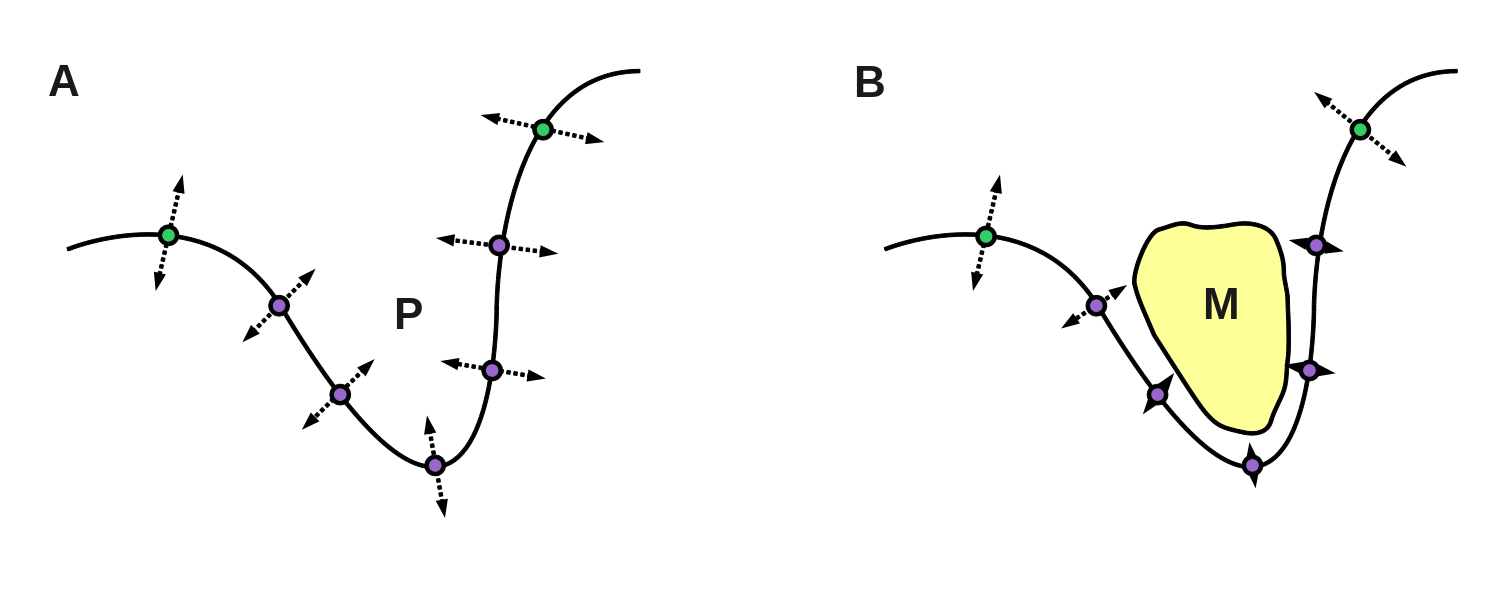
\includegraphics[width=\textwidth]{figures/ligand_binding/ligand_binding}

\caption[The change in flexibility of a protein on modulator binding at an allosteric site used as the basis for AlloPred]
{The change in flexibility of a protein on modulator binding at an allosteric site.
The black line indicates the surface of the protein and circles show residues: purple circles represent residues that are part of pocket P and green circles represent other residues.
Dashed arrows represent the magnitude of the fluctuations of a residue about equilibrium.
(A) shows the protein in the absence of a modulator.
All residues can vibrate.
(B) shows the effect of modulator M binding in pocket P.
The residues in the pocket have restricted motion and are less able to vibrate around their equilibrium positions.
Our method sought to approximate the effect of ligand binding by artificially restricting the flexibility of residues in a pocket using a higher spring constant in the elastic network.
Figure based on Figure~1 from Greener and Sternberg 2015 \cite{Greener2015}.}

\label{fig:ligand_binding}
\end{figure}


Once the perturbed NMA had been carried out, the degree of change caused by the perturbation needed to be measured.
Since changes at the active site will likely determine how strong an effect a modulator has, the effect of the perturbation on the active site should be considered.
Within each individual normal mode the effect of the perturbation was measured by averaging across all identified active site residues the magnitude of the difference between the perturbed and the unperturbed displacements from equilibrium.
This is shown visually in Figure~\ref{fig:nma_difference} and is given by:
$$
v_{i} = \frac{1}{N_{a}} \sum_{j=1}^{N_{a}} \left | \mathbf{p_{j}} - \mathbf{u_{j}} \right | = \frac{1}{N_{a}} \sum_{j=1}^{N_{a}} \left | \mathbf{d_{j}} \right |
$$

where $v_{i}$ is the effect of the perturbation in normal mode $i$, $\mathbf{p_{j}}$ is the displacement of residue $j$ in the perturbed normal mode, $\mathbf{u_{j}}$ is the displacement of residue $j$ in the unperturbed normal mode, $\mathbf{d_{j}}$ is the vector difference in the harmonic motion of residue $j$ before and after perturbation, and $N_{a}$ is the number of active site residues.


\begin{figure}
\centering

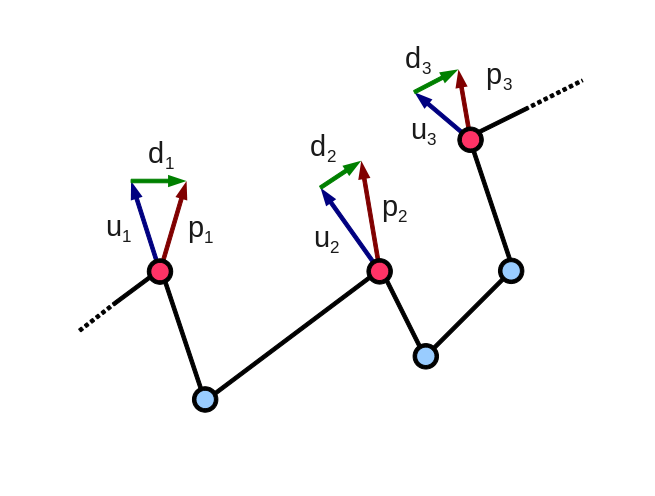
\includegraphics[width=0.5\textwidth]{figures/nma_difference/nma_difference}

\caption[Method used by AlloPred to calculate how much of an effect a change in the normal modes has at the active site]
{Diagram illustrating the method for calculating how much of an effect a change in the normal modes has at the active site.
The black lines represent the amino acid backbone of the protein.
Red circles represent amino acids identified as being active site residues; light blue circles represent other amino acids.
The dark blue arrows $\mathbf{u_{j}}$ represent the motion of C-alpha atoms in a particular normal mode before perturbation.
The brown arrows $\mathbf{p_{j}}$ represent the motion after perturbation at a particular pocket.
The differences $\mathbf{d_{j}}$ represent the vector difference between the motions, $\mathbf{d_{j}} = \mathbf{p_{j}} - \mathbf{u_{j}}$.
The differences are averaged across the active site, then a weighted average is taken across low-frequency normal modes to get a single numerical measure of the effect of the perturbation.}

\label{fig:nma_difference}
\end{figure}


The effects of the perturbation within each normal mode then needed to be averaged across the modes in order to get a single numeric measure for the strength of the effect arising from perturbation at one pocket.
The effect within each of the normal modes was weighted by the frequency such that the lowest-frequency mode of the chosen modes had the greatest influence on the results.
The equation to determine the effect of a perturbation $C_{m}$ is:
$$
C_{m} = \sum_{i=1}^{m} \frac{v_{i}}{\omega_{i}}
$$

where $v_{i}$ is defined above, $\omega_{i}$ is the frequency of mode $i$ and is hence equal to the square root of the eigenvalue $E_{i}$, and $m$ is the number of normal modes chosen for the calculation.
The justification for this method was that lower-frequency modes within the range selected are likely to be more important in allosteric communication because they consist of the long-range motions of many atoms \cite{Rodgers2013}.

It might be expected that larger pockets will have a higher $C_{m}$ value simply by virtue of having more residues perturbed.
In order to account for this a second measure, $E_{m}$, was defined as:
$$
E_{m} = \frac{C_{m}}{N_{p}}
$$

where $N_{p}$ is the number of residues in the pocket and $C_{m}$ was defined previously.
$E_{m}$ is a measure of the amount of change caused at the active site per residue in the perturbed pocket.
A Python script utilising the ProDy package \cite{Bakan2011} was used to perform NMA on the proteins.


\subsection{Machine learning}

Values of $C_{m}$ and $E_{m}$ with $m$ equal to 20, 50, 100, 200 and all modes were chosen as features in a SVM.
The features from the Fpocket output used in the SVM were:
\begin{itemize}
\item Rank
\item Score
\item Druggability score
\item Number of alpha spheres
\item Total SASA
\item Polar SASA
\item Apolar SASA
\item Volume
\item Mean local hydrophobic density
\item Mean alpha sphere radius
\item Mean alpha sphere solvent accessibility
\item Apolar alpha sphere proportion
\item Hydrophobicity score
\item Volume score
\item Polarity score
\item Charge score
\item Proportion of polar atoms
\item Alpha sphere density
\item Centre of mass - alpha sphere max distance
\item Flexibility
\end{itemize}

See the Fpocket documentation for more details on each of these measures.
Distance to the active site, number of residues in the pocket and number of pockets in the protein were also used as features.
The distance to the active site for each pocket was calculated as the distance between the geometric centre of the active site residues and the geometric centre of the residues in the pocket.
Each feature (apart from number of pockets) was utilised in two different ways: the feature value normalised across all proteins (\emph{raw}); and the ranking of the feature value within the values for that protein, where the ranks were scaled between 0 and 1 (\emph{ranked}).

The 65 features were ranked in Weka explorer \cite{Frank2004} using the ChiSquared attribute evaluator and the Ranker search method.
This evaluates the worth of a feature by computing the value of the chi-squared statistic with respect to the class.
The top 7 features only were retained, as features below this added little value.
The retained features, in descending order of descriptive power, were:
\begin{itemize}
\item Number of alpha spheres (raw)
\item $E_{200}$ (ranked)
\item Score (raw)
\item $E_{all}$ (ranked)
\item Distance to active site (raw)
\item Pocket size (raw)
\item Fpocket rank (raw)
\end{itemize}

The SVM-Light package \cite{Joachims1998} was used to run the SVM.
The Gaussian kernel was selected, containing internal parameters $C$ and $\gamma$.
The cost factor by which training errors on positive examples outweigh errors on negative examples was set as the ratio of negative to positive examples in the training set (6.19).
A leave-one-out parameterisation procedure was carried out over a grid of parameters with $C$ equal to 0.01, 0.1, 1 or 10 and $\gamma$ equal to $10^{-3}$, $10^{-4}$ or $10^{-5}$.
The procedure consisted of training the SVM on pockets from 78 of the 79 proteins in the training set and testing on pockets from the one left out.
The process was repeated for each protein in the set.
Performance was similar across the parameter range, with the parameters $C=1$ and $\gamma=10^{-4}$ being selected for the final SVM.
Due to the low number of allosteric pockets on each protein, only the top prediction was chosen as being allosteric.


\subsection{Web server}

A flowchart outlining the process of running a job is shown in Figure~\ref{fig:flowchart}.
The web server was implemented using the Django extension to Python and a SQLite database.
JSmol, a JavaScript implementation of the Jmol package, was used for molecular visualisation.
Bootstrap was used for page styling.
The standalone version of the code runs faster and it is recommended that users who intend to use the method extensively or in batch download the code for local use.


% define flowchart elements
\tikzstyle{process} = [rectangle, rounded corners, minimum width=3cm, minimum height=1cm, text width=2cm, text centered, draw=black, fill=orange!30]
\tikzstyle{input} = [trapezium, trapezium left angle=70, trapezium right angle=110, minimum width=3cm, minimum height=1cm, text width=2cm,, text centered, draw=black, fill=blue!30]
\tikzstyle{output} = [trapezium, trapezium left angle=70, trapezium right angle=110, minimum width=3cm, minimum height=1cm, text width=2cm,, text centered, draw=black, fill=red!30]
\tikzstyle{arrow} = [thick,->,>=stealth]

\begin{figure}
\centering
\singlespacing

\begin{small}
\begin{tikzpicture}[node distance=2cm]

\node (pdb) [input] {PDB ID/user file};
\node (nma) [process, below of=pdb] {Normal mode analysis};
\node (active) [input, left of=nma, xshift=-2cm] {Active site residues};
\node (fpocket) [process, right of=nma, xshift=2cm] {Fpocket calculation};
\node (svm) [process, below of=nma] {Run SVM};
\node (rerank) [process, below of=svm] {Re-rank allosteric pockets};
\node (visualisation) [output, right of=rerank, xshift=2cm] {Visualise pockets};
\node (download) [output, below of=rerank] {Download results};

\draw [arrow] (pdb) -| (fpocket);
\draw [arrow] (pdb) -- (nma);
\draw [arrow] (active) -- (nma);
\draw [arrow] (fpocket) -- (nma);
\draw [arrow] (fpocket) |- (svm);
\draw [arrow] (nma) -- (svm);
\draw [arrow] (svm) -- (rerank);
\draw [arrow] (rerank) -- (visualisation);
\draw [arrow] (rerank) -- (download);

\end{tikzpicture}
\end{small}

\caption[Flowchart showing the stages involved in running a job submitted to the AlloPred web server]
{Flowchart showing the stages involved in running a job submitted to the AlloPred web server.
Trapeziums represent inputs or outputs available to the user via the web front end (inputs purple, outputs red).
Rounded rectangles represent stages in the calculation pipeline that occur via the web back end.
Figure based on Figure~2 from Greener and Sternberg 2015 \cite{Greener2015}.}

\label{fig:flowchart}
\end{figure}


\section{Results}
\label{sec:allopred_results}

The AlloPred computational procedure, which uses NMA and other features to predict the allosteric pockets on a protein, was developed.
AlloPred models how the dynamics of a protein would be altered in the presence of a modulator at a specific pocket.
As described in Section... if the binding of a modulator causes a change in dynamics at the active site, it can be predicted to have an allosteric effect.
Pockets on the protein were first predicted using the Fpocket \cite{LeGuilloux2009} algorithm, which locates pockets using Voronoi tessellation and alpha spheres.
The normal modes of the protein were then calculated using the elastic network model, except the spring constant of any atom pair including a residue in a chosen pocket was set to be a higher value.
The effect of this perturbation was measured at the active site.
Intuitively, the interpretation of this change is that the binding of a small molecule in a pocket is expected to quench the vibrations of the surrounding residues.
These results were combined with output from Fpocket in a support vector machine (SVM) to predict allosteric pockets on proteins.

The AlloPred SVM was trained on a set of 79 known allosteric proteins (see the Methods section for selection criteria).
The top 7 retained features included 2 normal mode features, indicating the predictive power of normal mode perturbation.
AlloPred was tested on a test set of 40 known allosteric proteins.
For each protein AlloPred ranked the pockets and the top ranked pocket was examined.
For 23 of 40 proteins AlloPred ranked top a pocket containing an allosteric binding residue (an \emph{allosteric pocket}), when 18\% of pockets were allosteric pockets.
For 28 of 40 proteins an allosteric pocket was ranked first or second.
The results were compared to two existing methods for allosteric site prediction.
The AlloSite server uses the Fpocket algorithm and a machine learning approach \cite{Huang2013}, whereas the PARS server combines changes in protein flexibility and a structural conservation score \cite{Panjkovich2014}.
The correct predictions made by each method, and the overlap between the methods, are shown in Figure~\ref{fig:results_venn}.
AlloSite ranked an allosteric pocket top in 21 of 40 cases and is suitable for direct comparison to AlloPred as both methods rank pockets from Fpocket.
PARS, however, makes predictions of single points; a point was considered allosteric for our purposes if it was within 10 \AA\ of an allosteric modulator atom in the protein-modulator crystal structure.
It is important to note the different criteria for a correct prediction when considering the results.
PARS ranked an allosteric pocket top in 10 of 40 cases.
Figure~\ref{fig:results_venn} shows that AlloPred compares well to other methods and makes 4 correct predictions that neither of the other methods do.
This suggests that users of other allosteric prediction methods would benefit from the additional use of AlloPred.

In order to reduce the effects of bias during the split of the dataset into training and test sets, the dataset of 119 proteins was additionally split randomly 20 times into training and tests sets of 79 and 40 proteins respectively.
The SVM was then trained on the training set, using the previous parameters, and tested on the test set.
The average number of correct predictions across the 20 runs was 23.6 out of 40.
This shows that the above results used for comparison to other methods are indicative of the performance of the method.


\begin{figure}
\centering

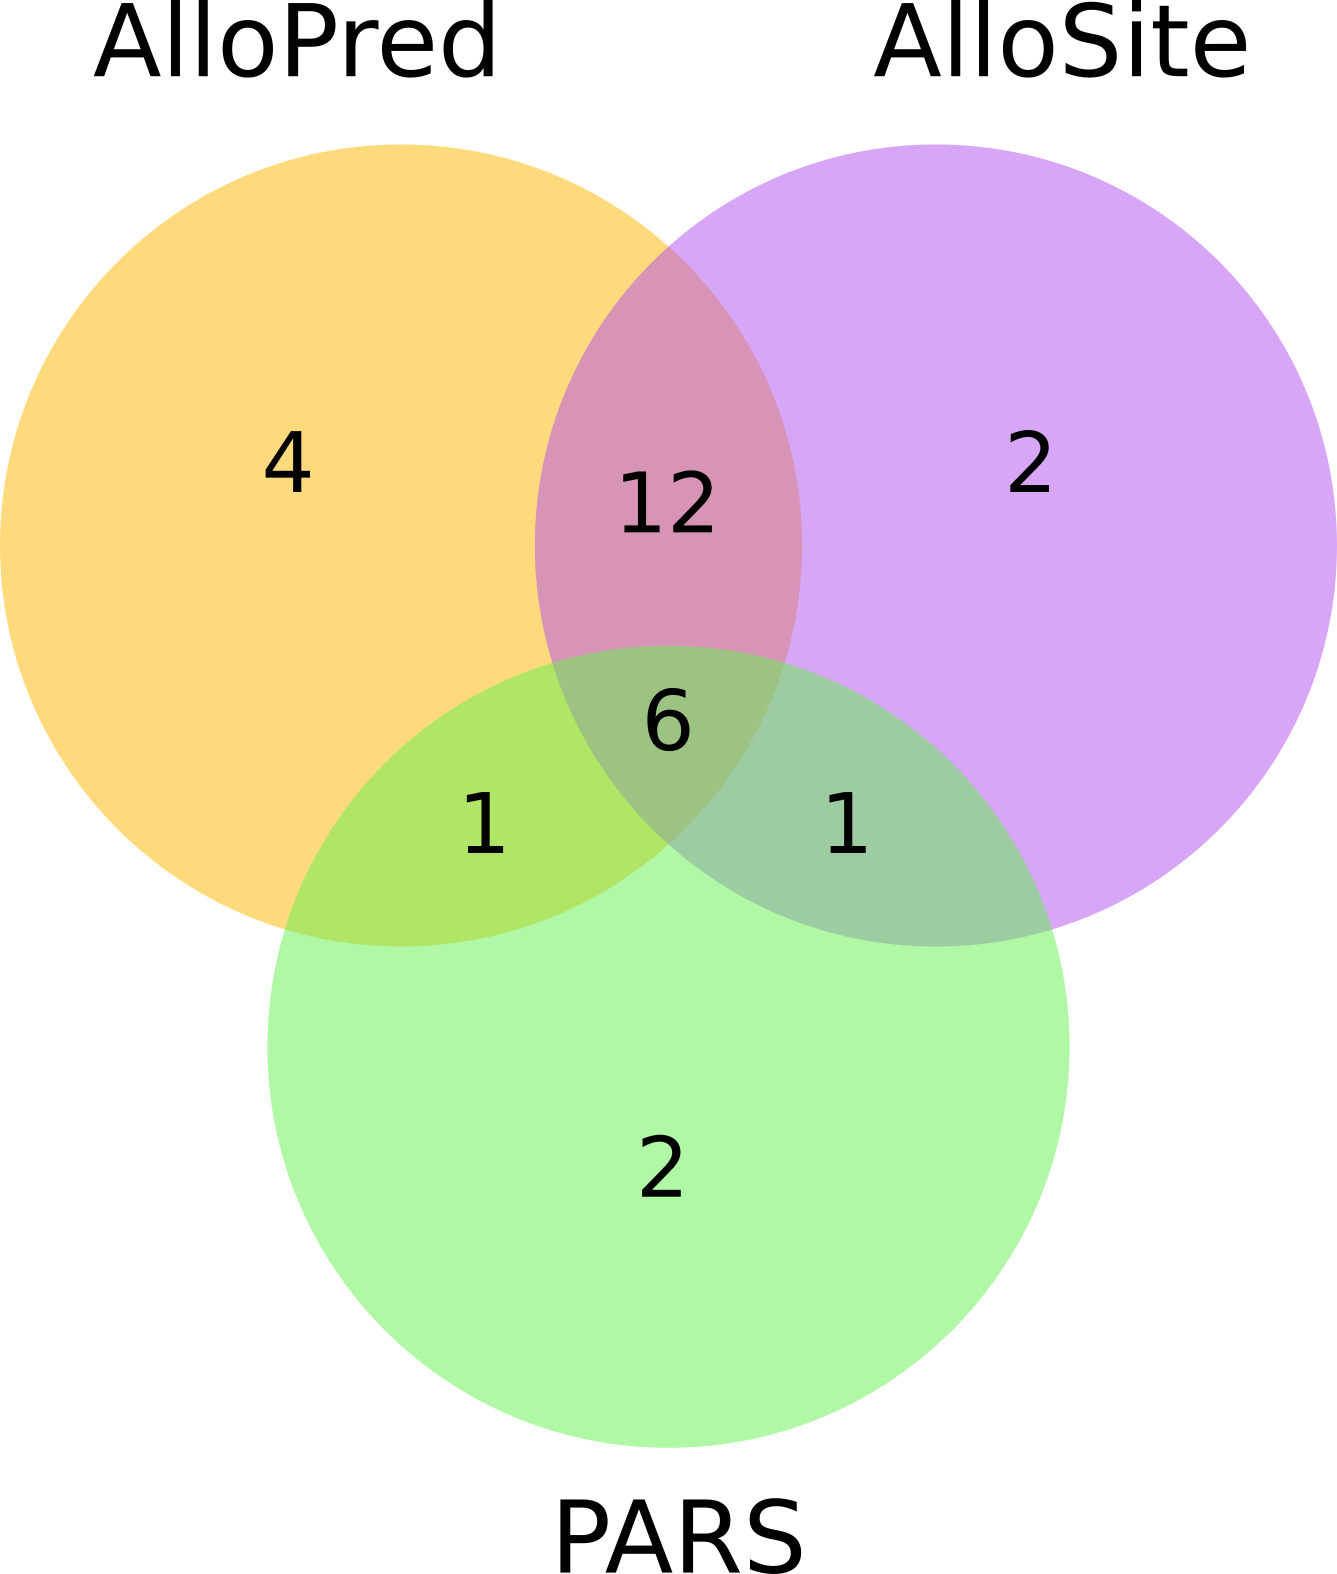
\includegraphics[width=0.5\textwidth]{figures/results_venn/results_venn}

\caption[Venn diagram comparing the performance of AlloPred on the test set to existing methods]
{Results comparison by method.
Venn diagram showing the number of top predictions for each protein by each method that were correct, from the test set of 40 proteins.
For AlloPred and AlloSite a correct prediction was prediction of a pocket containing at least one allosteric binding residue.
For PARS a correct prediction was prediction of a site within 10 \AA\ of at least one atom of the allosteric modulator in the protein-modulator crystal.
Figure based on Figure~3 from Greener and Sternberg 2015 \cite{Greener2015}.}

\label{fig:results_venn}
\end{figure}


\subsection{Web server}

The publicly-available AlloPred web server (\url{http://www.sbg.bio.ic.ac.uk/allopred/home}) allows users to analyse the prediction results via an intuitive interface.
Users can either input a PDB ID and chain(s) or upload a PDB file.
The active site residues of the protein must be given but there is an option to retrieve this data, if it is available, from the Catalytic Site Atlas (CSA, \url{http://www.ebi.ac.uk/thornton-srv/databases/CSA}) \cite{Furnham2014}.
The CSA has catalytic site data for around 70\% of enzymatic proteins in the PDB.
After submission a progress page shows the log file of the job and gives an estimated completion time.
When the results are available a link appears to the results page.
An example results page is shown in Figure~\ref{fig:web_results}.
All pockets are displayed in a table with their AlloPred rankings and Fpocket output.
The table can be sorted and filtered by any one or more of the 29 AlloPred and Fpocket features.
The page also allows users to visualise each pocket on the protein in a JSmol window that lets the user explore the protein and its predicted allosteric sites.
Features include highlighting the active site residues, selecting one of three visualisation options and a JSmol terminal to insert custom commands.
The results, including full details of each pocket, can be downloaded for further analysis as a tab-delimited text file.
The exploratory features on the website and results file containing all the pocket information set AlloPred apart from similar servers by allowing more extensive analysis of the results.
The calculation time is fast, with a 400 residue protein ($\sim$15 predicted pockets) analysed within 5 minutes.
The web server also includes a tutorial and a link to the source code to run AlloPred offline.


\begin{figure}
\centering


\includegraphics[width=0.8\textwidth]{figures/web_results/web_results}

\caption[Screenshots of the AlloPred web server results page]
{Screenshots of the AlloPred results page for the receptor-type adenylate cyclase with PDB ID 1FX2.
(A) The results table with default columns selected.
Three pockets have been chosen for visualisation.
(B) The JSmol window shown when the boxes are selected as in (A).
The ribbon visualisation option is used and the residues identified as being part of the active site are shown as balls and sticks.
Three pockets are shown in green, yellow and blue.
AlloPred correctly predicts the green pocket as being allosteric.
Figure based on Figure~4 from Greener and Sternberg 2015 \cite{Greener2015}.}

\label{fig:web_results}
\end{figure}


\section{Discussion}

Over the last few years a renewed interest in allostery, perhaps due to the potential benefits of allosteric drugs, has led to the development of a number of computational approaches to understanding allostery - see Section....
Some of these are directly associated with predicting allosteric sites on proteins from structure alone and are available as web servers that can take any PDB file as input.

The AlloSite server is similar to the method presented here in that it uses the Fpocket algorithm and attempts to elucidate allosteric pockets \cite{Huang2013}.
Whereas AlloSite solely uses the Fpocket output, our method uses an approach that combines flexibility with the Fpocket output.
A combination of methods may give better predictions than either method individually, as indicated by the unique predictions made by both methods during testing.
In fact the AlloSite predictions were found in every case to correspond to the pocket ranked top by Fpocket.
This highlights the difficulty in separating the prediction of allosteric sites from the prediction of binding sites in general.
It seems that Fpocket is able to predict good binding sites and AlloPred uses the extra flexibility information to bias this prediction towards sites with allosteric character.
% Be careful of repetition from introduction
The complete ranking of pockets provided by AlloPred may also be useful, as pockets ranked second were often found to be allosteric in the test set.

An approach that combines flexibility analysis using normal modes and structural conservation scores \cite{Panjkovich2012} is also similar to the method presented here and  was recently turned into a web server, PARS \cite{Panjkovich2014}.
Although direct comparison is difficult due to the differences in site calculation, definition of allosteric sites and datasets used, the method presented here again may be used well in combination as shown by Figure~\ref{fig:results_venn}.

The lack of input about the shape of the ligand and the large coverage of the protein in terms of pockets (average 18.5 pockets per protein) used by our method mean that it may be able to predict novel or unusual sites that methods which explicitly model the modulator might not.
This is important, for example when searching for allosteric sites on proteins believed to be non-allosteric.
Whilst the use of evolutionary information is clearly beneficial in allosteric prediction \cite{Reynolds2011} the use of structure alone is appealing for a general prediction method as it facilitates prediction of sites not currently conserved by evolution.
This is useful due to the large variety of allosteric modulators \cite{Wang2012} and mechanisms \cite{Motlagh2014}, suggesting potential novel modulators for proteins with known allosteric pathways.

Other promising approaches \cite{Demerdash2009, Kidd2009, Kaya2013} investigate the allosteric pathway and are not directly comparable with this method, which is only concerned with how the pathways transmit the effects of perturbations to the normal modes and does not directly reveal any information about the pathways themselves.
Again, a combination of our method with these approaches may be useful, as pockets predicted using our or other methods can be further investigated to reveal information about the underlying allosteric communication.

The main limitation of our method is related to the diversity found in allosteric systems.
Rigid-body motions of oligomers, side-chain dynamics, backbone motions and local unfolding are all mechanisms of allostery, with allosteric effects even present in intrinsically-disordered proteins \cite{Motlagh2014}.
A method based around the changes in dynamics on ligand binding is likely to miss many allosteric effects, and this can go some way to explaining the predictions of our method that were incorrect.
In particular, classic examples of allostery such as haemoglobin that involve oligomeric re-organisation to affect ligand cooperativity are not suitable for use with this method.
The method also relies upon knowledge of the active site location.
However, the results shown here and in other studies are encouraging and indicate a future where we can pick modulating sites on proteins with reasonable confidence.
Our method, for example, successfully predicts allosteric sites on proteins with a variety of sizes and functions.
The development of such methods that can be used by non-specialists without extensive parameter selection, and where the results are presented in a clear manner allowing exploration, will help bridge the gap between computational and experimental allosteric site prediction.


\chapter{ExProSE}
\label{cha:exprose}

This chapter describes ExProSE, a computational method based on distance geometry that generates an ensemble of protein structures from two input structures.
The structures span conformational space and the ensemble generation procedure can be perturbed to predict allosteric sites.
The work is further described in \cite{Greener2017}.


\section{Materials and Methods}
\label{sec:exprose_methods}

ExProSE is based on the CONCOORD distance geometry method \cite{DeGroot1997}, but has important differences that make it suitable for modelling conformational transitions and ensemble perturbations.
These are primarily the use of two input structures instead of one, a different procedure for achieving convergence, the ability to predict the effect of a modulator and an auto-parameterisation procedure.
ExProSE is implemented in Julia, a language that combines readable syntax similar to Python with performance approaching statically-compiled languages like C.
Work was initially begun in a combination of Python and C++ before switching to Julia.
Use of Julia allows good computational performance at the limiting steps, but also allows compact and easy-to-use code that others can modify.
The code, documentation, details of the datasets and instructions for reproducing the data are freely-available under the MIT license as a Julia package at \url{https://github.com/jgreener64/ProteinEnsembles.jl}.
The code is written in a modular way with associated unit tests and an automated building and testing procedure.


\subsection{Distance constraint generation}

The first step is to obtain a set of distance constraints from a protein structure.
Contrary to similar studies \cite{Panjkovich2012, Huang2013} the smallest biological assembly of the protein is used, rather than only the chain containing the allosteric modulator.
Hetero atom records, including the allosteric modulators, are removed.
Any existing hydrogens are removed and polar hydrogens are added using an in-house script.
Secondary structure assignments, required to obtain additional distance constraints, are obtained using the DSSP software \cite{Touw2015}.
As two structures for the same protein are utilised to generate distance constraints, only atoms common to both structures are used.
Every atom pair is examined and assigned an interaction type.
The criteria for each interaction are the same as in CONCOORD \cite{DeGroot1997} and are shown in Table~\ref{tab:interaction_types}.


\begin{sidewaystable}
\centering

\begin{small}
% Table generated by Excel2LaTeX from sheet 'interactions'
\begin{tabular}{ l l l p{10cm} }
\hline
\textbf{Number} & \textbf{Interaction name} & \textbf{Constraint tolerance / \AA} & \textbf{Definition} \\
\hline
1  & Covalent bond       & 0.02 & Pairs that are covalently bonded \\
2  & Bond angle          & 0.05 & Pairs where both atoms are covalently bonded to the same atom \\
3  & Ring                & 0.1  & Pairs that are part of ring systems \\
4  & Double bond 1-4     & 0.1  & 1-4 dihedral angle restricted pairs in side chain double bonds (found in ASN, GLN and ARG) \\
5  & Omega 1-4           & 0.1  & 1-4 pairs constrained by the rigid \textomega\ dihedral angle \\
6  & Tight phi/psi 1-4   & 0.2  & 1-4 pairs constrained by the \textphi /\textpsi\ dihedral angle where one residue is a proline or both residues are in the same helix/strand \\
7  & Loose phi/psi 1-4   & 0.4  & 1-4 pairs constrained by the \textphi /\textpsi\ dihedral angle where one residue is a glycine or both residues are in a loop region \\
8  & Other phi/psi 1-4   & 0.3  & 1-4 pairs constrained by the \textphi /\textpsi\ dihedral angle that do not fall into the above two categories \\
9  & Other 1-4           & 0.4  & Other 1-4 dihedral angle restricted pairs that do not fall into the above categories \\
10 & Secondary structure & 0.5  & Pairs of backbone atoms that are in the same helix/strand and are not more than 4 residues apart \\
11 & Salt bridge         & 0.75 & Pairs from oppositely-charged groups in close proximity (less than 4 \AA\ apart) \\
12 & Hydrogen bond       & 0.5  & Pairs that are part of a hydrogen bond; donor-acceptor distance is no more than 3.5 \AA, hydrogen-acceptor distance is no more than 2.5 \AA\ and the donor-hydrogen-acceptor angle is at least 90 degrees \\
13 & Tight hydrophobic   & 0.5  & Pairs where the interatomic distance is less than the sum of the van der Waals radii of the atoms plus 0.5 \AA; only C and H atoms are counted \\
14 & Loose hydrophobic   & 1    & Pairs where the interatomic distance is less than the sum of the van der Waals radii of the atoms plus 1.0 \AA; only C and H atoms are counted \\
15 & All other pairs     & 5    & Pairs that do not fall into any of the above categories \\
\hline
\end{tabular}
\end{small}

\caption{Interaction types between atom pairs.
These are the same as in CONCOORD \cite{DeGroot1997}.
The constraint tolerance values are used to generate lower and upper distance constraints between atoms.}

\label{tab:interaction_types}
\end{sidewaystable}


Each atom pair is assigned the first interaction for which it fulfils the criterion.
If an atom pair is not assigned any of the first 14 specific interactions, it is assigned the generic `All other pairs' interaction type.
Lower and upper distance constraints $l_{ij}$ and $u_{ij}$ are generated for each atom pair $ij$ based on the interatomic distance $d_{ij}$, the constraint tolerance for the interaction $t_{ij}$ and a tolerance weighting factor $W_{B}$ that is between 0.0 and 1.0:

$$
l_{ij} = d_{ij} - W_{B} t_{ij}, \quad u_{ij} = d_{ij} + W_{B} t_{ij}
$$

The selection of $W_{B}$ is described below.
For example two atoms 1.54 \AA\ apart and in a covalent bond with $W_{B}$ equal to 0.5 would have a lower distance constraint of 1.53 \AA\ and an upper distance constraint of 1.55 \AA, as the constraint tolerance multiplied by $W_{B}$ is 0.01 \AA.
This process yields a set of distance constraints for each crystal structure of a protein.

The distance constraints generated from the two structures for the same protein are combined to get a set of combined constraints.
The constraints are combined in such a way that the new constraints for a given atom pair cover the distance of both the individual constraints for that pair.
For example if two atoms have a lower and upper distance constraint of 6.0 \AA\ and 7.0 \AA\ in structure one, and 6.5 \AA\ and 7.5 \AA\ in structure two, then the new constraints will be 6.0 \AA\ and 7.5 \AA.
This is shown visually in Figure~\ref{fig:distance_constraints}.


\begin{figure}
\centering

%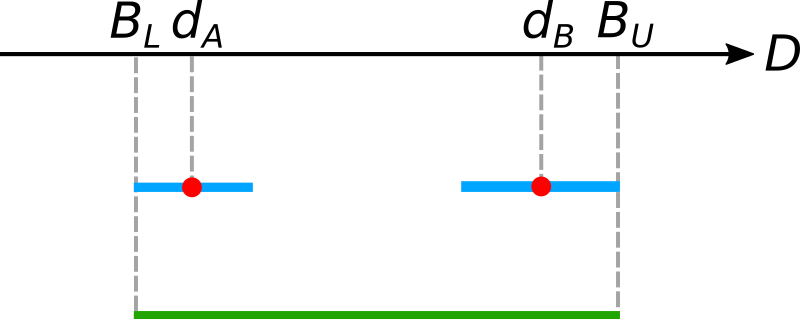
\includegraphics[width=0.7\textwidth]{figures/distance_constraints/distance_constraints}

\caption{The method to calculate the upper and lower distance constraints between two atoms given two input protein structures.
First, the distance between the two atoms in each of the two input structures is calculated ($d_{A}$ and $d_{B}$).
An upper and lower distance constraint is then calculated for each of these distances by multiplying the constraint tolerance for the interaction in that structure by the tolerance weighting factor (these constraints are shown as blue bars).
The upper and lower limits of these constraints are combined to get the new distance constraints $B_{U}$ and $B_{L}$ (green bar).}

\label{fig:distance_constraints}
\end{figure}


It is undesirable to retain all the `All other pairs' interactions (type 15 in Table~\ref{tab:interaction_types}) as they vastly outnumber the specific interactions (types 1-14).
Specific interactions scale with the atom number $N_{A}$ whereas other pairs scale as $N_{A}^{2}$.
Hence only a fraction of the other pairs are retained as distance constraints.
The probability of retaining an other pair is chosen so that the final number of other pairs is roughly $20N_{A}$, the value used by studies utilising CONCOORD \cite{DeGroot1999}.

$W_{B}$ is chosen for each protein in the apo/holo and allosteric datasets by a process of auto-parameterisation.
$W_{B}$ equal to 0.0 usually results in a narrow range of structures that are midway between the two input structures.
By contrast, $W_{B}$ equal to 1.0 usually results in structures that cover a wide conformational space beyond the input structures.
A measure for the conformational spread of the ensemble was developed.
This measure $F$ is the fraction of structures $S$ in the ensemble for which $TM(S,A) > TM(B,A)$ and $TM(S,B) > TM(A,B)$ where $TM(X,Y)$ is the TM-score between model $X$ and reference $Y$, and $A$ and $B$ are the two input crystal structures.
The TM-score is a measure of similarity between two protein structures.
$F$ therefore gives the proportion of structures that are closer to both input structures than the input structures are to each other.
$F$ equal to 0.9 indicates an ensemble that effectively covers the conformational space of the input structures.
Ensembles of 50 structures are generated with $W_{B}$ starting at 1.0 and decreasing in steps of 0.1.
When the ensemble generated has an $F$ value of at least 0.9, that $W_{B}$ is chosen.
For the specific examples T4-lysozyme and CDK2, $W_{B}$ is equal to 0.2 and 0.3 respectively.
It should be noted that the above auto-parameterisation procedure to select $W_{B}$ is implemented automatically and requires no input by the user.
For CAP only one input structure is used so $W_{B}$ is selected manually as 0.4.
This value allows flexibility in the ensemble whilst giving good quality structures.


\subsection{Protein structure generation}

Once the distance constraints have been generated, an iterative process is used to generate structures that satisfy the constraints.
Stochastic Proximity Embedding (SPE) \cite{Agrafiotis2013} was selected, as it has been shown to converge effectively and scales well with system size.
This procedure provides better convergence than the CONCOORD procedure of moving atoms to a random distance within the distance constraints.
The pseudocode for the SPE algorithm, rephrased from an existing review \cite{Agrafiotis2013}, is shown in Algorithm~\ref{algorithm:spe}.
The distance constraints do not include favourability for a particular chirality, so coordinates produced from SPE are examined and structures with the incorrect chirality are reversed by mirroring all coordinates in the $xy$ plane.


\begin{algorithm}[p]
\caption{SPE algorithm}
\label{algorithm:spe}
\begin{algorithmic}

\State Define lower and upper distance constraints $l_{ij}$ and $u_{ij}$ for atom pairs $i$ and $j$
\State Define an initial learning rate $\lambda_{d} = 1.0$
\State Randomise atomic coordinates $x_{i}$ within a cube of 100 \AA
\For{$C$ cycles}
    \For{$S$ steps}
        \State Randomly select a pair of atoms $i$ and $j$ for which a constraint exists
        \State Compute the distance $d_{ij} = \left\| x_{i} - x_{j} \right\|$
        \If{$d_{ij} < l_{ij}$ or $d_{ij} > u_{ij}$}
            \State Update the coordinates $x_{i}$ and $x_{j}$ by
                $$
                x_{i} = x_{i} + \frac{\lambda_{d}}{2} \frac{t_{ij} - d_{ij}}{d_{ij}} (x_{i} - x_{j})
                $$
                $$
                x_{j} = x_{j} + \frac{\lambda_{d}}{2} \frac{t_{ij} - d_{ij}}{d_{ij}} (x_{j} - x_{i})
                $$
            \State where $t_{ij}$ is the nearest constraint to $d_{ij}$
        \EndIf
    \EndFor
    \State Decrease the learning rate $\lambda_{d}$ by $1 / C$
\EndFor

\end{algorithmic}
\end{algorithm}


Once a set of coordinates has been generated, an SPE error score can be calculated that measures how well the distance constraints are satisfied \cite{Agrafiotis2013}.
This score is calculated as shown in Algorithm~\ref{algorithm:scoring}.
Structures with a high error score tend to have more violations of allowed stereochemistry, which is to be expected as there are more violations of allowed constraints.
In order to account for this, more structures are generated than required and those with the highest scores are discarded.
The ratio is set to be 1.5.
So if the final ensemble had 200 structures, initially 300 are generated and the 100 with the highest error score are discarded.
This was found during development to generally produce ensembles of structures with acceptable stereochemical quality.


\begin{algorithm}[p]
\caption{Scoring algorithm}
\label{algorithm:scoring}
\begin{algorithmic}

\State Set score $s = 0$
\For{each atom pair $i$, $j$ with a distance constraint}
    \If{$d_{ij} < l_{ij}$ or $d_{ij} > u_{ij}$}
        \State Increase $s$ by
        $$
        \frac{(d_{ij} - t_{ij})^{2}}{\max \left ( u_{ij} - l_{ij}, 0.001 \right )}
        $$
        \State where $t_{ij}$ is the nearest constraint to $d_{ij}$
    \EndIf
\EndFor

\end{algorithmic}
\end{algorithm}


The number of iterations per atom, the product of the number of cycles $C$ and the number of steps $S$ from Algorithm~\ref{algorithm:spe}, is taken as 60,000.
This was chosen as the SPE error score did not generally decrease for iterations beyond this.
The ratio of $S$ to $C$ is taken as 50:1 as in practice any value of $S > C$ will give similar results \cite{Agrafiotis2013}.
The reduction in learning rate over the course of the minimisation makes this process similar to simulated annealing.
Initially large movements through the conformational space allow the correct region to be found.
The movements are dampened over time to allow the system to converge to a solution.
This procedure is carried out separately multiple times to obtain an ensemble.


\subsection{Ensemble analysis}

Ensembles of structures produced are iteratively aligned following the procedure described in the methodology of a previous study \cite{Bakan2009}.
This aligns an ensemble without the use of a reference structure.
The average structure of the ensemble is taken as the centroid of the coordinates across the ensemble following this superimposition.

PCA is carried out on the generated ensemble.
The coordinates across the ensemble are compared to the average coordinates and a set of orthogonal motions are found that describe the variation in the ensemble.
The covariance matrix $C_{ij}$ is a matrix where $i$ and $j$ represent the indices of the $3 N_{C}$ atomic coordinates of the $N_{C}$ C\textsuperscript{\textalpha} atoms.
$C_{ij}$ is calculated as
$$
C_{ij} = \langle (x_{i} - \langle x_{i} \rangle) \cdot (x_{j} - \langle x_{j} \rangle) \rangle
$$
where the averages in angle brackets are over the ensemble and $x$ represents the atomic coordinates.
$C$ is then diagonalised to yield the PCs.


\subsection{Modulator constraint generation}

In order to predict how a modulator binding to the protein affects the distribution of structures in conformational space, additional distance constraints representing the modulator need to be generated.
Potential binding sites are predicted using LIGSITE\textsuperscript{\it cs} \cite{Huang2006}, which is a development of the original LIGSITE algorithm \cite{Hendlich1997}.
Additional constraints are generated based on pocket points predicted by LIGSITE\textsuperscript{\it cs}.
In order to keep the number of additional points the same for pockets of different sizes, 120 points are chosen randomly.
If fewer than 120 points are predicted by LIGSITE\textsuperscript{\it cs}, points are re-sampled.
Using 120 points was found for CDK2 and CAP to add enough constraints to potentially alter the distribution of the ensemble and see an effect, but not so many that invalid structures are produced.
Changing this parameter changes the strength of the perturbations but does not generally change the ranking of pockets by RMSD (see below).
For CAP a different procedure was used as the location of the bound cAMP molecules is known from the crystal structure.
In this case 120 fake points are added at 1.2 \AA\ gaps in a ball around the location of the C1' atom in cAMP, while the cAMP molecules are themselves omitted from the simulation.
Selected points have distance constraints of tolerance 0.1 \AA\ with all protein atoms within 7 \AA.
% NtrC phosphorylation here
Addition of the new distance constraints leads to ensembles that may differ significantly from the unperturbed ensemble.

In the allosteric prediction procedure ensembles are generated with additional constraints (termed `perturbation') at selected pockets in turn, then compared to the original `unperturbed' ensemble.
Each pocket greater than a size cutoff of 13 \AA\textsuperscript{3} is selected, up to a maximum of 8 pockets per protein.
Below this size a small-molecule modulator is unlikely to have enough space to bind.
8 pockets gives a reasonable sampling of the surface of a protein and generally includes all sizeable pockets.
The C$\alpha$ RMSD between the average structure in the unperturbed ensemble and the average structure in the perturbed ensemble is used to compare ensembles.
This RMSD is used to rank the perturbed pockets in terms of their predicted allosteric nature (largest to smallest RMSD).
This RMSD measure may seem simplistic but gave similar or superior performance to statistical measures, such as the Mann-Whitney $U$ test on the ensemble fluctuations between the unperturbed and perturbed ensembles, during development.
A pocket is considered allosteric for validation purposes if the pocket centre is within 6 \AA\ of at least one atom of the modulator defined as the allosteric modulator in the ASD.
This is similar to previous studies \cite{Panjkovich2012}.


\subsection{Apo/holo dataset}

Out of the 25 proteins used in a prior study \cite{Atilgan2010}, the 12 with apo/holo all-atom RMSD greater than 2 \AA\ are selected in order to focus on larger conformational changes.


\subsection{Allosteric dataset}

All 150 proteins in the ASD \cite{Shen2016} with apo and holo structures available in the PDB are examined.
58 proteins with apo and holo structures are selected using the following criteria: (i) apo/holo all-atom RMSD greater than 0.25 \AA, (ii) TM-score greater than 0.5 and (iii) no more than two chains and 1,000 residues in the smallest biological assembly.
Proteins are also clustered by sequence identity at a threshold of 30\%, with representatives being the proteins with the highest apo/holo RMSD, to remove similar proteins.


\subsection{Method comparison}

\subsubsection{Ensemble generation}

tCONCOORD \cite{Seeliger2007} is run with default parameters.
NMSim is run via the NMSim web server \cite{Kruger2012} with the default parameters for large scale motions.
This produces 5 trajectories of 500 structures. Every tenth structure is taken from each trajectory to yield representative ensembles of 250 structures.
Alternative parameters for tCONCOORD and NMSim are used to generate the results in Figure~\ref{fig:method_params} and these are described in the figure.


\subsubsection{Molecular dynamics}

All MD runs are carried out using the GROMACS package \cite{Abraham2015}.
Energy minimisation to improve the stereochemistry of T4-lysozyme structures is conducted using a steepest descent energy minimization of 5000 steps in a vacuum and the OPLS-AA force field.
MD runs of T4-lysozyme are conducted using periodic boundary conditions, SPC water, charge-neutralizing counter ions, the OPLS-AA force field and a 2 fs timestep.
An initial energy minimisation is followed by a constant temperature and volume equilibration for 100 ps, then a constant pressure and temperature equilibration for 100 ps.
MD is run for 50 ns.
PLUMED \cite{Tribello2014} with GROMACS is used to carry out targeted MD.
C$\alpha$ RMSD to the target structure is used as a collective variable with a $\kappa$ value starting at 0 $\textup{kJ} \: \textup{mol}^{-1} \: \textup{\AA}^{-2}$ and increasing linearly to 1000 $\textup{kJ} \: \textup{mol}^{-1} \: \textup{\AA}^{-2}$ over 10 ps, and remaining at this value for the rest of the run.


\subsubsection{Allosteric site prediction}

LIGSITE\textsuperscript{\it cs} \cite{Huang2006} and Fpocket \cite{LeGuilloux2009} are run with default parameters.
The procedure for determining if an Fpocket pocket is allosteric is as follows: the average of the locations of the vertices in the pocket is taken as the pocket centre, and the pocket is considered allosteric if this centre was within 6 \AA\ of at least one atom of the modulator defined as the allosteric modulator in the ASD.
This is consistent with the criterion for determining LIGSITE\textsuperscript{\it cs} allosteric pockets defined previously.
PARS results are obtained by using the PARS web server \cite{Panjkovich2014}.
PARS uses LIGSITE\textsuperscript{\it cs}, so the same criterion as LIGSITE\textsuperscript{\it cs} is used to determine allosteric pockets.
AlloPred is run using the offline version \cite{Greener2015} and default parameters.
The active site residues are retrieved from the Catalytic Site Atlas (CSA) \cite{Furnham2014}, or from literature inspection when not available in the CSA.
AlloPred uses Fpocket, so the same criterion as Fpocket is used to determine allosteric pockets.
STRESS \cite{Clarke2016} is run offline using the source code.
Since the output of STRESS is pocket residues, a pocket is called as allosteric if there is at least one modulator atom within 3 \AA\ of any atom in the given residues of the pocket.
This represents the modulator being close to part of the predicted pocket.
This value of 3 \AA\ is less than the value of 6 \AA\ used previously as there are many residues which the modulator can be close to, rather than a single pocket centre.


\subsubsection{Computation time}

ExProSE generates 250 structures in $\sim$20 minutes for T4-lysozyme on a 3.1 GHz Intel Core i7 processor.
For tCONCOORD the time is $\sim$10 minutes.
NMSim is run via the NMSim web server and takes $\sim$5 hours.
MD and targeted MD use considerably more resources, with a 50 ns run taking $\sim$60 hours on 16 cores (2.3 GHz Intel Xeon CPU E5-2698) or $\sim$20 days on the single processor above.

The ExProSE computation time is significantly improved over initial attempts due to optimisiation of the Julia code.
Comparison of the performance-critical step (moving the atoms to satisfy the distance constraints) shows it is significantly faster that the same algorithm implemented in simple Python.
The stochastic nature of the simulation means it is not easily amenable to vectorisation in NumPy.
The performance-critical step in Julia showed speed around 1.5 times slower than an implementation in C.


\section{Results}
\label{sec:exprose_results}

The motivation for developing ExProSE was to explore allostery in the framework of the protein structural ensemble.
% Ref to into diagram
A method was needed that could use existing structural information to generate ensembles that spanned the large conformational changes relevant in allostery.
We decided to extend the popular existing method tCONCOORD.
tCONCOORD converts a protein structure to a series of distance constraints based on chemical interactions (e.g.\ hydrogen bonds) then uses an iterative procedure to move randomly-placed atoms to satisfy the distance constraints.
We alter this by using two structures as input, meaning the structures generated can span the conformational space spanned by the input structures.
There are also other important differences to tCONCOOD (see methods).

ExProSE is able to (i) generate ensembles of protein structures from two input structures and (ii) predict allosteric pockets on proteins.
First, the use of ExProSE is exemplified and explored on a protein kinase with a hinge opening motion.
It is then shown using a dataset of structural pairs that two widely-used methods for generating ensembles cannot span large conformational changes, whereas ExProSE can.
The ability of ExProSE to produce native-like ensembles is exemplified with T4-lysozyme.
ExProSE ensembles can be perturbed to reveal the location of allosteric sites, as demonstrated on cyclin-dependent kinase 2 (CDK2).
The performance of ExProSE in predicting allosteric sites is assessed on a dataset of 58 known allosteric proteins and compared to existing methods.
Finally, a well-studied example of dynamic allostery is examined.


\subsection{Ensemble generation}

\subsubsection{Adenylate kinase}

Adenylate kinase is... hinge opening...
Importance of parameterisation and how this can be a problem with existing methods/MD.
SPE score minimisation over time.
Important parameter in ExProSE.
Desire to control it.
Fig shows ensemble spread with different parameters and set chosen by auto-parameterisation.
This method used throughout.

% Modify
It is instructive to examine the convergence of the structural generation simulations.
The SPE error score is a measure of how many distance constraints are violated.
Figure~\ref{fig:spe_convergence} shows the SPE error score over the course of the iterative constraint correcting process for 5 independent runs of CDK2 structure generation.
It can be seen that 60,000 iterations per atom is enough for the structure to improve as much as it can.
Further iterations beyond this do not have a meaningful effect on the SPE error score.
Similar convergence behaviour was seen with proteins across a variety of sizes.


\begin{figure}
\centering

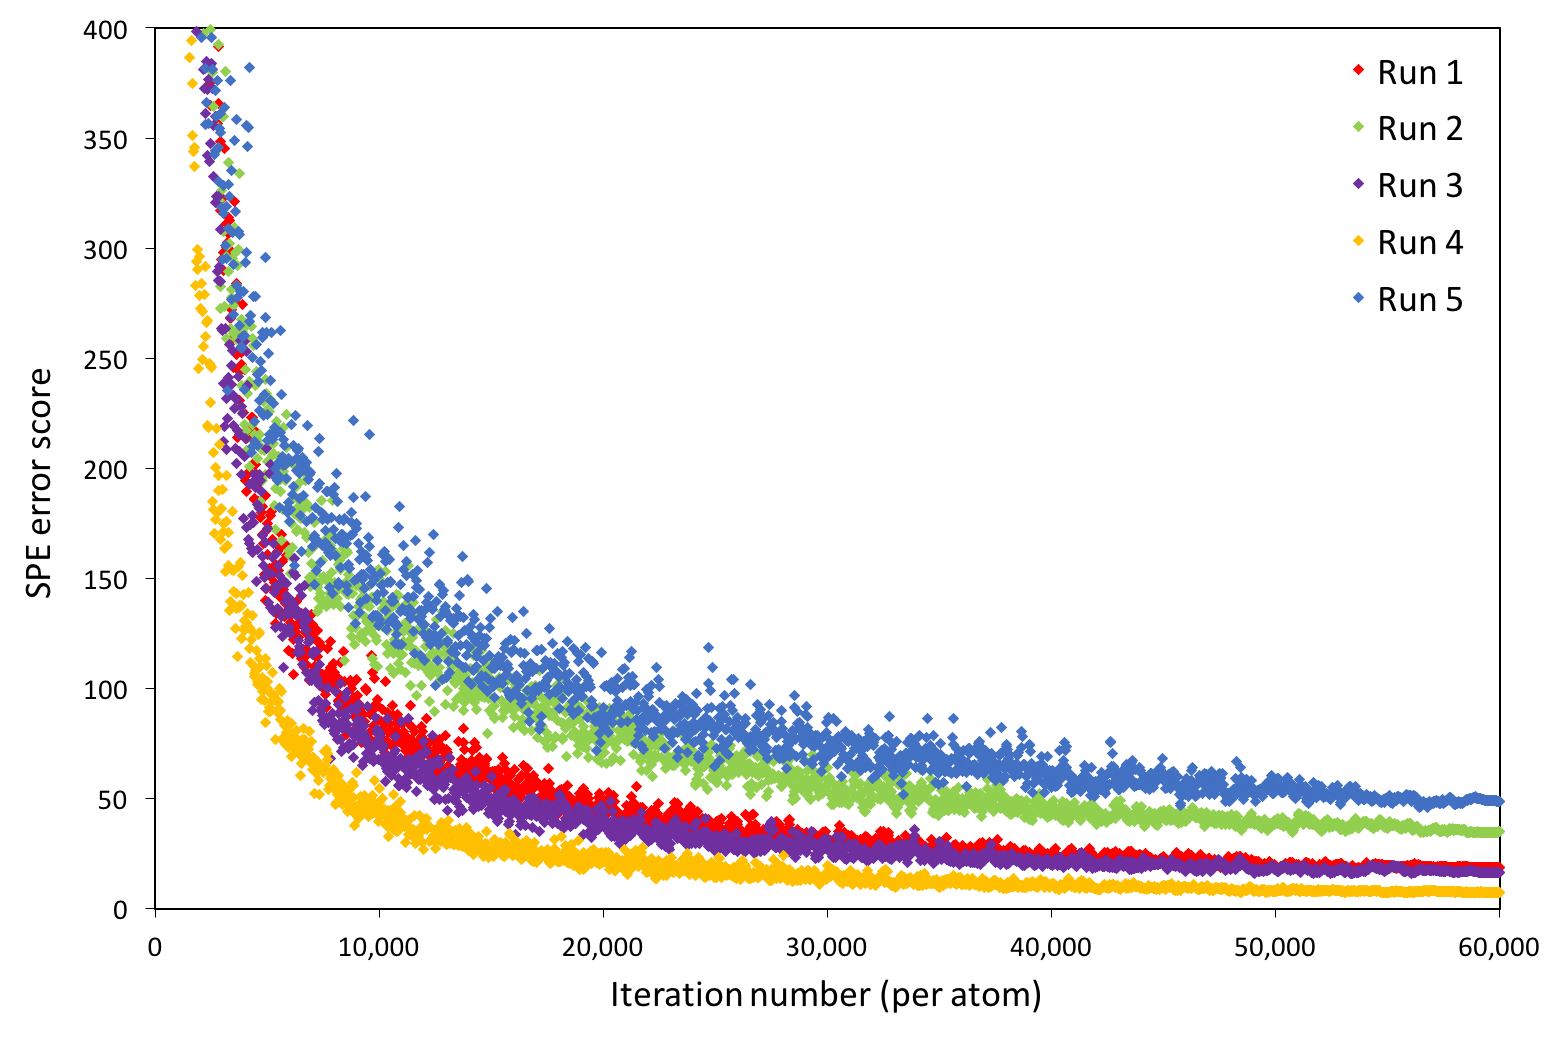
\includegraphics[width=\textwidth]{figures/spe_convergence/spe_convergence}

\caption{The SPE error score, a measure of how many distance constraints are violated, shown over the course of 5 separate runs on CDK2.
Initially the random atomic coordinates give a high score.
As the iterative procedure occurs atoms that violate distance constraints are moved, reducing the SPE error score.}

\label{fig:spe_convergence}
\end{figure}


\subsubsection{Apo/holo dataset}

In order to examine the ability of existing non-MD methods to generate ensembles that span conformational changes, a dataset of apo (no modulator) and holo (modulator bound) structures was used \cite{Atilgan2010}.
The proteins have RMSD between apo and holo structures ranging from 2 \AA\ to 19 \AA, and represent a variety of domain, subdomain and subunit motions.
tCONCOORD \cite{Seeliger2007} and NMSim \cite{Kruger2012} both seek to model conformational changes such as those in the dataset.
Default parameters were used to produce 250 structures for each protein from tCONCOORD and NMSim.
The lowest RMSD of the structures in an ensemble to a particular crystal structure was taken as a measure of how close the ensemble came to exploring the conformational space of that crystal structure.
This can be seen in Table~\ref{tab:ensemble_dataset}.

When the apo structure is used as input, structures similar to the apo structure are generated by both methods.
The median lowest RMSD to the apo crystal is 1.44 \AA\ for tCONCOORD and 0.71 \AA\ for NMSim.
However, structures similar to the holo crystal are not sampled.
The median lowest RMSD to the holo crystal is 4.15 \AA\ for tCONCOORD and 4.68 \AA\ for NMSim.
In a similar manner, when the holo structure is used as input to tCONCOORD and NMSim the ensembles sample the holo structure but not the apo structure.

ExProSE, as expected because it uses both the apo and holo crystals as input, is able to generate structures close to both crystals - see Table~\ref{tab:ensemble_dataset_ex}.
For 11 out of the 12 proteins ExProSE can generate a structure closer to the holo crystal than the other methods, where the other methods use the apo structure as input.
For the opposite case, comparing to the apo crystal, ExProSE also generates a closer structure for 11 out of 12 proteins.
Hence ExProSE is useful for generating ensembles when two or more structures are available.

PROCHECK checks the stereochemical quality of protein structures \cite{Laskowski1993}.
The PROCHECK overall G-factor is a log-odds score based on the observed distributions of various stereochemical parameters in reference proteins.
A lower overall G-factor represents a low-probability conformation, and indicates a less stereochemically-valid structure.
Ideally, scores should be above -0.5, and values below -1.0 may need investigation \cite{Esposito2006}.
The median PROCHECK overall G-factor across all generated structures is -0.99 for ExProSE, indicating that PROCHECK produces structures that are generally acceptable.
The values for NMSim and tCONCOORD are -0.32 and -1.83 respectively, indicating that NMSim produces good quality structures and tCONCOORD produces structures with poor stereochemical quality.
The stereochemistry of generated structures can be improved by energy minimisation (see below).


\begin{sidewaystable}
\centering

\begin{small}
% Table generated by Excel2LaTeX from sheet 'methods'
\begin{tabular}{rrrrrllllllll}
\hline
      &       &       &       &       & \multicolumn{2}{c}{\textbf{tCONCOORD}} & \multicolumn{2}{c}{\textbf{tCONCOORD}} & \multicolumn{2}{c}{\textbf{NMSim}} & \multicolumn{2}{c}{\textbf{NMSim}} \\
      &       &       &       &       & \multicolumn{2}{c}{\textbf{from apo}} & \multicolumn{2}{c}{\textbf{from holo}} & \multicolumn{2}{c}{\textbf{from apo}} & \multicolumn{2}{c}{\textbf{from holo}} \\
      &       &       &       &       & \multicolumn{8}{c}{Lowest RMSD from 250 generated structures to apo/holo crystal / \AA} \\
\multicolumn{1}{l}{\textbf{Protein name}} & \multicolumn{1}{l}{\textbf{Apo PDB}} & \multicolumn{1}{l}{\textbf{Holo PDB}} & \multicolumn{1}{l}{\textbf{RMSD / \AA}} & \multicolumn{1}{l}{\textit{\textbf{N}}} & \textbf{Apo} & \textbf{Holo} & \textbf{Apo} & \textbf{Holo} & \textbf{Apo} & \textbf{Holo} & \textbf{Apo} & \textbf{Holo} \\
\hline
\multicolumn{1}{l}{OxyR transcription factor} & \multicolumn{1}{l}{1I6A} & \multicolumn{1}{l}{1I69} & \multicolumn{1}{l}{2.44} & \multicolumn{1}{l}{206} & 1.18  & 2.69  & 2.66  & 1.12  & 1.04  & 2.61  & 2.51  & 0.72 \\
\multicolumn{1}{l}{Ferric binding protein}    & \multicolumn{1}{l}{1D9V} & \multicolumn{1}{l}{1MRP} & \multicolumn{1}{l}{2.68} & \multicolumn{1}{l}{309} & 1.22  & 1.81  & 1.88  & 1.41  & 0.62  & 2.07  & 2.31  & 0.71 \\
\multicolumn{1}{l}{Aspartate receptor}        & \multicolumn{1}{l}{1LIH} & \multicolumn{1}{l}{2LIG} & \multicolumn{1}{l}{2.77} & \multicolumn{1}{l}{157} & 1.16  & 2.73  & 2.94  & 1.48  & 0.94  & 2.45  & 2.65  & 0.80 \\
\multicolumn{1}{l}{HIV-1 rev. transcriptase}  & \multicolumn{1}{l}{2HMI} & \multicolumn{1}{l}{3HVT} & \multicolumn{1}{l}{3.81} & \multicolumn{1}{l}{555} & 2.49  & 4.11  & 4.66  & 3.44  & 0.64  & 3.28  & 3.14  & 0.78 \\
\multicolumn{1}{l}{Maltose binding protein}   & \multicolumn{1}{l}{1OMP} & \multicolumn{1}{l}{3MBP} & \multicolumn{1}{l}{3.88} & \multicolumn{1}{l}{370} & 0.97  & 2.62  & 2.66  & 0.89  & 0.71  & 2.35  & 2.39  & 0.57 \\
\multicolumn{1}{l}{Small G protein Arf6}      & \multicolumn{1}{l}{1E0S} & \multicolumn{1}{l}{2J5X} & \multicolumn{1}{l}{4.44} & \multicolumn{1}{l}{164} & 0.99  & 4.18  & 4.23  & 0.96  & 0.66  & 4.00  & 4.23  & 0.86 \\
\multicolumn{1}{l}{Immunoglobulin}            & \multicolumn{1}{l}{1MCP} & \multicolumn{1}{l}{4FAB} & \multicolumn{1}{l}{5.95} & \multicolumn{1}{l}{214} & 1.65  & 3.60  & 3.80  & 1.51  & 0.62  & 5.35  & 3.63  & 0.79 \\
\multicolumn{1}{l}{Myosin}                    & \multicolumn{1}{l}{1VOM} & \multicolumn{1}{l}{2AKA} & \multicolumn{1}{l}{6.23} & \multicolumn{1}{l}{730} & 2.60  & 5.11  & 5.63  & 2.38  & 0.73  & 5.53  & 5.77  & 0.63 \\
\multicolumn{1}{l}{Adenylate kinase}          & \multicolumn{1}{l}{4AKE} & \multicolumn{1}{l}{1AKE} & \multicolumn{1}{l}{7.19} & \multicolumn{1}{l}{214} & 1.70  & 4.88  & 6.00  & 1.18  & 0.58  & 6.16  & 6.09  & 0.74 \\
\multicolumn{1}{l}{Serpin}                    & \multicolumn{1}{l}{1PSI} & \multicolumn{1}{l}{7API} & \multicolumn{1}{l}{8.96} & \multicolumn{1}{l}{372} & 1.20  & 8.71  & 8.93  & 1.51  & 0.71  & 8.22  & 8.97  & 0.97 \\
\multicolumn{1}{l}{GroEL}                     & \multicolumn{1}{l}{1AON} & \multicolumn{1}{l}{1OEL} & \multicolumn{1}{l}{12.6} & \multicolumn{1}{l}{524} & 3.01  & 9.72  & 9.61  & 2.45  & 0.87  & 10.8  & 10.1  & 0.48 \\
\multicolumn{1}{l}{Topoisomerase II}          & \multicolumn{1}{l}{1BGW} & \multicolumn{1}{l}{1BJT} & \multicolumn{1}{l}{18.8} & \multicolumn{1}{l}{664} & 3.36  & 17.5  & 17.0  & 3.34  & 0.81  & 18.0  & 17.3  & 0.65 \\
\hline
\multicolumn{5}{r}{\textbf{Median across all proteins}} & 1.44  & 4.15  & 4.45  & 1.50  & 0.71  & 4.68  & 3.93  & 0.73 \\
\hline
\end{tabular}
\end{small}

\caption{Comparison of ensemble generation methods.
The columns Apo PDB and Holo PDB refer to the PDB IDs of the apo and holo structures used.
RMSD is the all-atom RMSD in \AA\ between the apo and holo structures.
The rows are ordered by increasing RMSD.
\textit{N} is the number of residues in common between the apo and holo chains used.
The values on the right are the lowest RMSD in \AA\ of the structures in an ensemble produced using the method and input indicated, to the crystal structure indicated.
A low value indicates that the ensemble sampled a structure close to the crystal structure.
The median of the lowest RMSDs for each method/input combination is also given.}

\label{tab:ensemble_dataset}
\end{sidewaystable}


\begin{table}
\centering

\begin{small}
% Table generated by Excel2LaTeX from sheet 'exprose'
\begin{tabular}{rrrrrll}
\hline
      &       &       &       &       & \multicolumn{2}{c}{Lowest RMSD from 250 generated ExProSE structures to apo/holo crystal / \AA} \\
\multicolumn{1}{l}{\textbf{Protein name}} & \multicolumn{1}{l}{\textbf{Apo PDB}} & \multicolumn{1}{l}{\textbf{Holo PDB}} & \multicolumn{1}{l}{\textbf{RMSD / \AA}} & \multicolumn{1}{l}{\textit{\textbf{N}}} & \textbf{Apo} & \textbf{Holo} \\
\hline
\multicolumn{1}{l}{OxyR transcription factor} & \multicolumn{1}{l}{1I6A} & \multicolumn{1}{l}{1I69} & \multicolumn{1}{l}{2.44} & \multicolumn{1}{l}{206} & 1.02  & 1.16 \\
\multicolumn{1}{l}{Ferric binding protein}    & \multicolumn{1}{l}{1D9V} & \multicolumn{1}{l}{1MRP} & \multicolumn{1}{l}{2.68} & \multicolumn{1}{l}{309} & 0.90  & 1.08 \\
\multicolumn{1}{l}{Aspartate receptor}        & \multicolumn{1}{l}{1LIH} & \multicolumn{1}{l}{2LIG} & \multicolumn{1}{l}{2.77} & \multicolumn{1}{l}{157} & 1.25  & 0.88 \\
\multicolumn{1}{l}{HIV-1 rev. transcriptase}  & \multicolumn{1}{l}{2HMI} & \multicolumn{1}{l}{3HVT} & \multicolumn{1}{l}{3.81} & \multicolumn{1}{l}{555} & 1.84  & 1.45 \\
\multicolumn{1}{l}{Maltose binding protein}   & \multicolumn{1}{l}{1OMP} & \multicolumn{1}{l}{3MBP} & \multicolumn{1}{l}{3.88} & \multicolumn{1}{l}{370} & 0.85  & 1.50 \\
\multicolumn{1}{l}{Small G protein Arf6}      & \multicolumn{1}{l}{1E0S} & \multicolumn{1}{l}{2J5X} & \multicolumn{1}{l}{4.44} & \multicolumn{1}{l}{164} & 1.70  & 1.88 \\
\multicolumn{1}{l}{Immunoglobulin}            & \multicolumn{1}{l}{1MCP} & \multicolumn{1}{l}{4FAB} & \multicolumn{1}{l}{5.95} & \multicolumn{1}{l}{214} & 3.90  & 5.33 \\
\multicolumn{1}{l}{Myosin}                    & \multicolumn{1}{l}{1VOM} & \multicolumn{1}{l}{2AKA} & \multicolumn{1}{l}{6.23} & \multicolumn{1}{l}{730} & 2.38  & 1.89 \\
\multicolumn{1}{l}{Adenylate kinase}          & \multicolumn{1}{l}{4AKE} & \multicolumn{1}{l}{1AKE} & \multicolumn{1}{l}{7.19} & \multicolumn{1}{l}{214} & 3.15  & 1.98 \\
\multicolumn{1}{l}{Serpin}                    & \multicolumn{1}{l}{1PSI} & \multicolumn{1}{l}{7API} & \multicolumn{1}{l}{8.96} & \multicolumn{1}{l}{372} & 1.08  & 1.01 \\
\multicolumn{1}{l}{GroEL}                     & \multicolumn{1}{l}{1AON} & \multicolumn{1}{l}{1OEL} & \multicolumn{1}{l}{12.6} & \multicolumn{1}{l}{524} & 3.13  & 3.70 \\
\multicolumn{1}{l}{Topoisomerase II}          & \multicolumn{1}{l}{1BGW} & \multicolumn{1}{l}{1BJT} & \multicolumn{1}{l}{18.8} & \multicolumn{1}{l}{664} & 3.54  & 5.10 \\
\hline
\multicolumn{5}{r}{\textbf{Median across all proteins}} & 1.77  & 1.69 \\
\hline
\end{tabular}
\end{small}


\caption{Ability of ExProSE ensembles to reach apo and holo structures.
The columns Apo PDB, Holo PDB, RMSD and \textit{N} are the same as in Table~\ref{tab:ensemble_dataset}.
The values on the right are the lowest RMSD in \AA\ of the structures in an ExProSE ensemble to the crystal structure indicated.
A low value indicates that the ensemble sampled a structure close to the crystal structure.
The median of the lowest RMSDs is also given.}

\label{tab:ensemble_dataset_ex}
\end{table}


\subsubsection{T4-lysozyme}

Here, we demonstrate that ExProSE can generate structures close to crystals not used as input.
Lysozymes damage bacterial cell walls by catalysing the hydrolysis of peptidoglycans.
Bacteriophage T4-lysozyme is a suitable protein for analysing conformational variability as there are many crystal structures available and MD simulations of the protein have shown that simulations up to 200 ns do not reliably reach both the open and closed conformations \cite{Seeliger2007}.
The pairwise RMSDs of the crystals range from 0.64 \AA\ to 4.25 \AA.

An ensemble was generated using ExProSE from the open (PDB ID 169L, chain E) and closed (PDB ID 2LZM) conformations.
Four random structures from this ensemble are shown compared to the open and closed crystal structures in Figure~\ref{fig:t4l}A.
Principal components analysis (PCA) can be carried out on an ensemble of structures to find the orthogonal motions that describe the variation in the ensemble.
Figure~\ref{fig:t4l}B shows the projections of the generated ensemble and the 38 crystal structures used in a prior study \cite{DeGroot1998} onto the first and second principal components (PCs), which account for 70\% and 12\% of the motion respectively.
The dominant first eigenvector corresponds to opening and closing of the structure.
It can be seen that the method is able to sample conformations corresponding to experimentally-observed structures, as the ensembles largely overlap.

Ensembles produced by tCONCOORD starting from the open and closed structures separately are shown in Figure~\ref{fig:t4l}C.
As demonstrated previously on other proteins, the ensemble generated from the open structure cannot reach all the way to the closed structure, and vice versa.
The tCONCOORD ensembles also sample structures not found in the ensemble of crystal structures, particularly when using the open conformation as input.
This tendency of tCONCOORD to produce ensembles with too much structural variability was also noted by the authors \cite{Seeliger2009}.

Ensembles produced by NMSim starting from the open and closed structures separately are shown in Figure~\ref{fig:t4l}D.
In this case, the ensemble generated from the open and closed structures can largely span the conformational space.
Similar to tCONCOORD, regions not explored by the crystals are sampled by NMSim.
For example, there is one model in the ensemble generated from the open structure that has an RMSD of 7.38 \AA\ to the nearest crystal structure.

Alternative parameters were also used for tCONCOORD and NMSim to see how the ensembles varied - see Figure~\ref{fig:method_params}.
For tCONCOORD decreasing the upper bound for long range constraints, and/or turning off close pairs as constraints, had little effect on the distribution of the ensembles.
For NMSim using the parameters for small scale motions led to ensembles that could not span the conformational space.
In each case the default parameters gave similar or better coverage of the conformational space of the crystals by visual inspection, and were hence used for the analysis below.


\begin{figure}
\centering

%\includegraphics[width=\textwidth]{figures/t4l}

\caption{T4-lysozyme ensembles.
(\textbf{A}) Four structures generated from ExProSE using the open (PDB ID 169L, chain E)  and closed (PDB ID 2LZM) conformations as input are shown in orange.
The crystal structures of the open and closed conformations are shown in blue and green respectively for reference.
The arrow shows the opening motion caused by the breaking of a hydrogen bond between ARG137 and GLU22.
(\textbf{B}) Projections of the 38 crystal structures used in a prior study \cite{DeGroot1998} onto the first (x-axis) and second (y-axis) PCs of the PCA of the crystal structures, which account for 70\% and 12\% of the motion respectively (black dots).
Projections from the ensembles generated with ExProSE are also shown (red dots).
(\textbf{C}) Projections of two tCONCOORD ensembles on the same plot as (B).
An ensemble using the open structure as input (blue dots) and an ensemble using the closed structure as input (yellow dots) are shown.
(\textbf{D}) Projections of two NMSim ensembles with parameters for large scale motions on the same plot as (B).
An ensemble using the open structure as input (blue dots) and an ensemble using the closed structure as input (yellow dots) are shown.}

\label{fig:t4l}
\end{figure}


\begin{figure}
\centering

%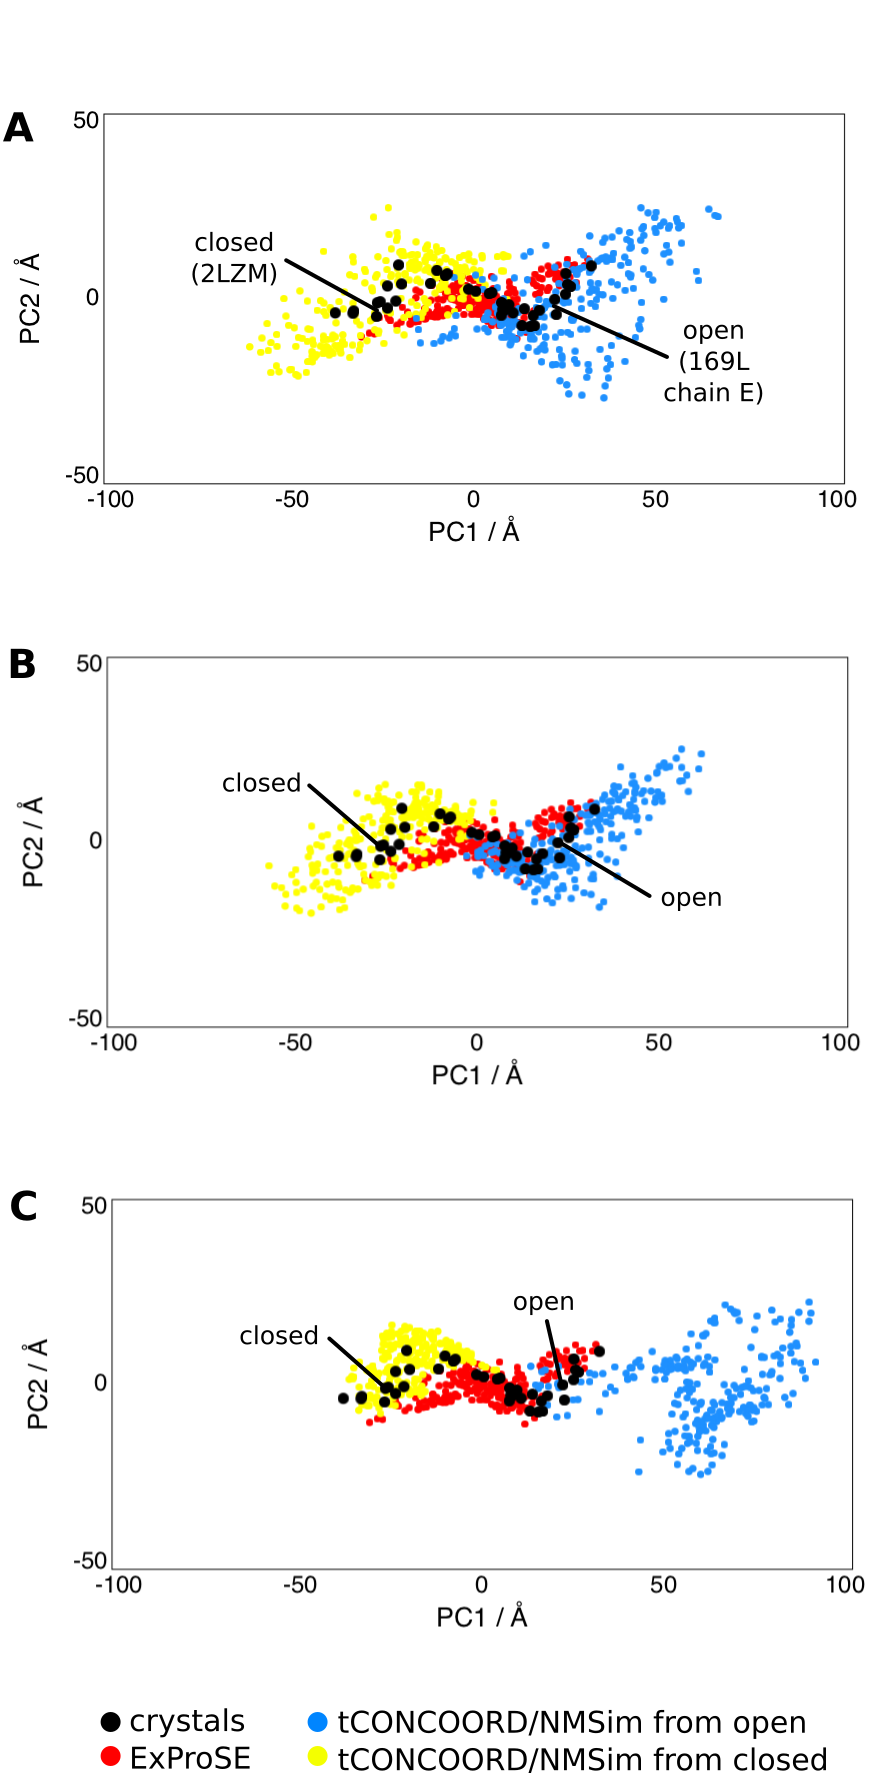
\includegraphics[width=\textwidth]{figures/method_params}

\caption{Ensemble generation for T4-lysozyme with different parameters.
Projections of tCONCOORD/NMSim ensembles from the open (blue dots) and closed (yellow dots) structures onto the PCA of the crystal structures are shown.
Similar to Figure~\ref{fig:t4l}, in each graph the projections of the crystals (black dots) and projections from the ensembles generated with ExProSE (red dots) are also shown.
(A) tCONCOORD ensembles with the upper bound for long range constraints set to 1.3 \AA\ (default 2.0 \AA ).
(B) tCONCOORD ensembles with the upper bound for long range constraints set to 1.3 \AA\ and close pairs not used as constraints.
(C) NMSim ensembles using the default parameters for small scale motions.}

\label{fig:method_params}
\end{figure}


T4-lysozyme was also studied with MD.
50 ns MD runs starting from the closed conformation were not able to reach the open conformation and vice versa - see Figure~\ref{fig:t4l_md}A and \ref{fig:t4l_md}B.
Targeted MD runs starting from the closed conformation and targeting the open conformation (and vice versa) were also carried out.
In targeted MD the atoms are guided to a target structure with the use of a steering force that seeks to minimise the RMSD of the structure to the target structure.
These ensembles can be seen in Figure~\ref{fig:t4l_md}C and \ref{fig:t4l_md}D, and are generally able to cross conformational space over the course of around 20 ns.
However beyond this time they show unpredictable behaviour and can deviate from the experimental structures.
Retaining only the structures up to 20 ns, as in Figure~\ref{fig:t4l_md}C and \ref{fig:t4l_md}D, gives ensembles that largely overlap with the experimental structures.


\begin{figure}
\centering

%\includegraphics[width=\textwidth]{figures/t4l_md}

\caption{MD T4-lysozyme ensembles.
Projections of two repeats of a particular MD run onto the PCA of the crystal structures are shown (blue and yellow dots), with snapshots taken every 100 ps.
Similar to Figure~\ref{fig:t4l}, in each graph the projections of the crystals are also shown (black dots).
(\textbf{A}) 50 ns MD runs starting from the closed structure (PDB ID 2LZM).
(\textbf{B}) 50 ns MD runs starting from the open structure (PDB ID 169L).
(\textbf{C}) 20 ns targeted MD runs starting from the closed structure and targeting the open structure.
(\textbf{D}) 20 ns targeted MD runs starting from the open structure and targeting the closed structure.}

\label{fig:t4l_md}
\end{figure}


By combining tCONCOORD, NMSim and targeted MD ensembles generated using the open and closed structures as input, a fair comparison to ExProSE can be made.
A generated ensemble should ideally contain models close to all the crystal structures.
The degree to which this occurs for ExProSE ensembles, and combined ensembles for tCONCOORD, NMSim and targeted MD up to 20 ns, is shown in Figure~\ref{fig:t4l_rmsd}A.
It can be seen that ExProSE is able to generate structures close to all crystals, with all crystals having an RMSD of 1.7 \AA\ or less to a generated structure.
For 26 out of 38 crystals ExProSE generates a model closer to the crystal than NMSim.
It generates a closer model than tCONCOORD in all cases.
For 15 out of 38 crystals ExProSE generates a model closer to the crystal than targeted MD.
However, this is the case for 14 out of the 27 structures that have an RMSD of more than 1.0 \AA\ to both the open and closed reference structures.
Of these 27, ExProSE performs better for all of the 4 structures that have an RMSD of more than 1.5 \AA.
Hence ExProSE is able to generate better models than the other methods for crystals which are far from either input structure, as seen on the right side of Figure~\ref{fig:t4l_rmsd}A.
The PROCHECK overall G-factor of the closest models for each method is shown in Figure~\ref{fig:t4l_rmsd}B.
ExProSE is able to produce models of acceptable quality close to all the crystals, even for those further from the input structures.

In order to determine whether the stereochemical quality of generated structures could be improved, energy minimisation was carried out on all structures.
For all methods, energy minimisation improved median PROCHECK overall G-factors.
Across the ensembles the median values increased from the range [-2.23, -0.45] to the range [-0.31, -0.17] - see Table~\ref{tab:energy_minimisation}.
This shows that stereochemical problems in generated structures can in general be improved by energy minimisation, important if using generated structures for docking studies.

By using two input structures rather than one, ExProSE is able to produce models of acceptable quality close to other crystal structures.
It can explore conformational space better than methods that use a single structure as input.


\begin{figure}
\centering

%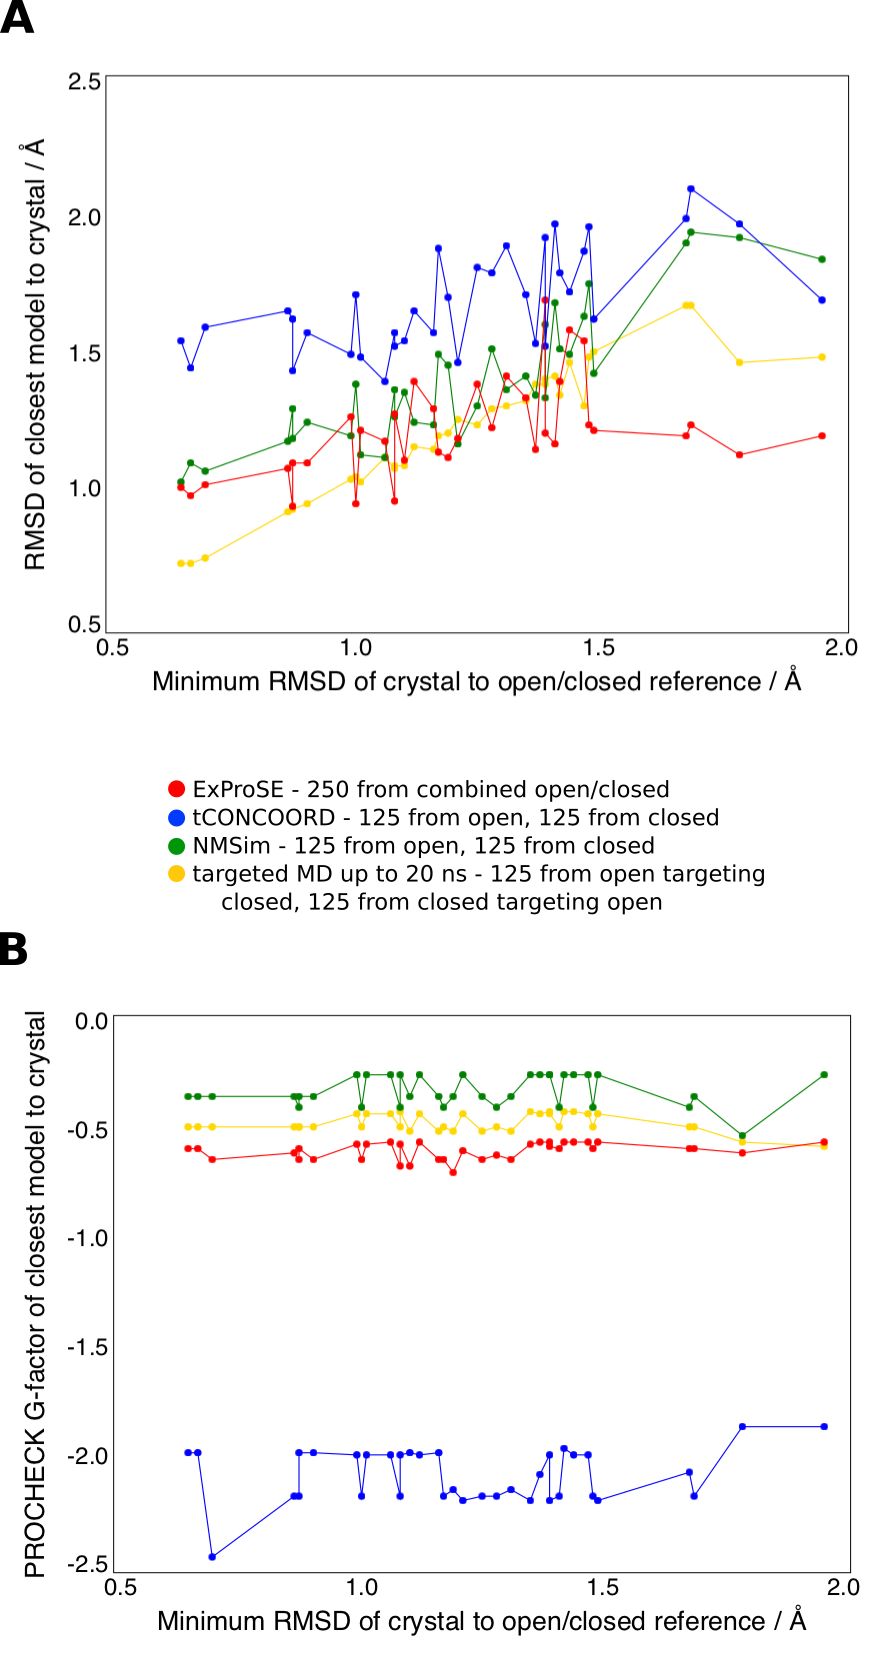
\includegraphics[width=0.5\textwidth]{figures/t4l_rmsd}

\caption{Closest models from each ensemble to T4-lysozyme crystal structures.
(\textbf{A}) The RMSD of the closest model from each generated ensemble to the crystal structures.
The crystal structures are sorted by the lower of the two RMSD values to the open and closed crystals used as input.
The crystals used as inputs are omitted from the graph.
(\textbf{B}) PROCHECK overall G-factors of the closest model from each generated ensemble to the crystal structures.
The crystal structures are sorted as in (A).}

\label{fig:t4l_rmsd}
\end{figure}


\begin{table}
\centering

\begin{scriptsize}
% Table generated by Excel2LaTeX from sheet 'minimise'
\begin{tabular}{ l l p{4cm} p{4cm} }
\hline
\textbf{Method} & \textbf{Strucure(s) used} & \textbf{Median overall G-factor\newline before energy minimisation} & \textbf{Median overall G-factor\newline after energy minimisation} \\
\hline
ExProSE     & open and closed                 & -0.58 & -0.26 \\
tCONCOORD   & open                            & -2.23 & -0.31 \\
tCONCOORD   & closed                          & -2.09 & -0.27 \\
NMSim       & open                            & -0.50 & -0.31 \\
NMSim       & closed                          & -0.45 & -0.29 \\
targeted MD & starting open, targeting closed & -0.56 & -0.17 \\
targeted MD & starting closed, targeting open & -0.57 & -0.20 \\
\hline
\end{tabular}
\end{scriptsize}

\caption{Improvement in stereochemical quality on energy minimisation.
The structures in each ensemble were analysed with PROCHECK and the median overall G-factor across the ensemble was noted.
The median of the overall G-factor of each structure after energy minimisation was also recorded.}

\label{tab:energy_minimisation}
\end{table}


\subsection{Ensemble perturbation for CDK2}

Here, we demonstrate that ExProSE ensembles can be perturbed to reveal modulating sites.
CDK2 is a protein kinase essential for the G1/S phase transition in the cell cycle - see (section ref).
An ExProSE ensemble was generated using the apo native structure (PDB ID 1HCL) and the holo structure bound to two ANS molecules in an allosteric site (PDB ID 3PXF).
The ANS-bound structure is inactive, as ANS binding causes a conformational shift in the C-helix that prevents cyclin binding \cite{Betzi2011}.
A further screening study has found potential modulators for the ANS binding site \cite{Rastelli2014}.

Figure~\ref{fig:cdk}A shows the pockets predicted by LIGSITE\textsuperscript{\it cs} \cite{Huang2006} on CDK2 bound to two ANS molecules.
The ensemble perturbation procedure was carried out at each of the 8 pocket centres as described in the experimental procedures.
In brief, additional constraints are added representing a modulator bound in the selected pocket.
Projections of the structures of the unperturbed ensemble and the structures of the ensemble with perturbation at the pocket centre are shown in Figure~\ref{fig:cdk}B, one graph per pocket centre.
The third PC was chosen for visualisation instead of the second as it represents the inactivating motion of the C-helix, whereas the second PC represents a rotation in the region of the protein considered to be functionally less important, the C-lobe.

Site 1 in Figure~\ref{fig:cdk}A and \ref{fig:cdk}B is the ANS allosteric pocket.
Simulating a modulator there shifts the ensemble towards the inactive state, agreeing with previous experimental data \cite{Betzi2011}.
Site 2 is the ATP-binding site and there is no change in the ensemble by simulating a modulator there.
This is encouraging as ATP binding does not cause structural changes that lead to cyclin dissociation.
Site 3 is found in a pocket near the activation segment.
A shift in the ensemble towards the inactive state is seen on perturbation at this site.
In fact this site is close to a potential allosteric site suggested in another computational study \cite{Pitt2014}, and is part of the region associated with cyclin-binding.
This indicates that the site could potentially be an allosteric site, though further effort would be required to determine whether it is druggable.
Simulating modulators at sites 4 to 8 does not shift the ensemble, suggesting that binding at these sites is unable to cause an allosteric effect.
No allosteric modulators have been reported experimentally for these sites.


\begin{figure}
\centering

%\includegraphics[width=\textwidth]{figures/cdk}

\caption{CDK2 pockets and projections of ensembles.
(\textbf{A}) CDK2 in its holo conformation bound to two ANS molecules in the allosteric site (PDB ID 3PXF).
CDK2 is shown as a green cartoon with the two bound ANS shown as blue sticks.
Pocket centres predicted by LIGSITE\textsuperscript{\it cs} are shown as purple spheres.
The pockets are numbered by descending volume.
Pocket 1 represents the ANS allosteric pocket.
Pocket 2 represents the ATP binding pocket.
(\textbf{B}) Structures generated using ExProSE, with input structures the apo and holo structures (PDB ID 1HCL and 3PXF respectively), are shown as red dots.
The axes are projections onto the first (x-axis) and third (y-axis) PCs of the ExProSE ensemble, which account for 35\% and 8\% of the motion respectively.
The blue dots represent the structures in the ensemble with perturbation at pocket centres 1-8 from (A).}

\label{fig:cdk}
\end{figure}


\subsection{Allosteric site prediction}

Systematic methods to predict allosteric sites on proteins are necessary to utilise the potential advantages of allosteric drugs.
A diverse dataset of 58 apo/holo pairs representing the unbound protein and the protein bound to a known allosteric modulator was assembled from the ASD \cite{Shen2016}.
This dataset showed a large range in protein size (153 to 955 residues) and included a variety of proteins including transcriptional regulators, transporters and protein kinases.

LIGSITE\textsuperscript{\it cs} was used to predict pockets on the holo crystal structures and ExProSE was used to generate a perturbed ensemble for each pocket centre as described in the experimental procedures.
These perturbed ensembles were used to rank the pockets in terms of predicted allosteric effect.
In this study a correct prediction for a protein indicates that an allosteric pocket was ranked first or second.
This criterion was chosen as a measure of success because typically the top few pockets predicted by a method would be examined and studied further.

The ability of ExProSE to predict allosteric pockets on the dataset is compared to existing allosteric prediction methods, which are run with the holo crystal structures as input.
This was found to give better results for the existing methods than using the apo crystals.
PARS \cite{Panjkovich2014} uses NMA with and without a predicted modulator to predict changes in flexibility.
STRESS \cite{Clarke2016} is an implementation of the earlier binding leverage algorithm \cite{Mitternacht2011}, which models how perturbations due to binding couple to the motions of the protein as expressed by low-frequency normal modes.
AlloPred \cite{Greener2015} uses perturbation of normal modes and pocket features in a machine learning approach to predict allosteric pockets.
It should be noted that different criteria are used to define an allosteric pocket for each method, due to the nature of their output - see the experimental procedures.
For 27 of 58 proteins ExProSE ranked an allosteric pocket first or second, performing better than the other three methods.
This is shown in Table~\ref{tab:allosteric_methods}.
Only 7 proteins have an allosteric pocket ranked first or second by all four methods.
In 3 cases ExProSE makes a correct prediction for a protein while none of the other methods did.

The performance of the allosteric prediction methods is also compared to the pocket prediction methods LIGSITE\textsuperscript{\it cs} and Fpocket \cite{LeGuilloux2009} in Table~\ref{tab:allosteric_methods}.
LIGSITE\textsuperscript{\it cs} and Fpocket are effective at finding allosteric sites, both ranking an allosteric pocket first or second for 31 out of 58 proteins, even though they are not designed specifically for allosteric site prediction.
This is not too surprising as the holo structures were used as input, so the modulator had a reasonable chance of being in one of the two largest pockets.
However ExProSE is still valuable as it finds smaller, less obvious allosteric pockets.
This could be due to the extra structural information used as input.
For example, ExProSE in 6 cases finds sites not ranked in the top 2 by LIGSITE\textsuperscript{\it cs} and in 8 cases finds sites not ranked in the top 2 by Fpocket.
ExProSE shows the best complementarity to the pocket prediction methods along with STRESS, which makes fewer correct predictions.
ExProSE also gives information on how the ensemble may be affected by the modulators, as demonstrated in Figure~\ref{fig:cdk}, allowing inspection of the predicted structural and dynamic changes arising from perturbation.

The performance on each protein by each method is shown in Table~\ref{tab:allosteric_proteins}.
This is to our knowledge the first systematic comparison of multiple allosteric prediction methods.
49 of 58 proteins had an allosteric pocket ranked first or second by at least one of the 6 methods compared in Table~\ref{tab:allosteric_methods}.
This complementarity indicates the potential for a meta approach that combines predictions from multiple methods.


\begin{table}
\centering

% Table generated by Excel2LaTeX from sheet 'summary'
\begin{tabular}{ p{3cm} p{3cm} p{3cm} p{3cm} }
\hline
\textbf{Method} & \textbf{Correct in top 2\newline (out of 58)} & \textbf{Unique from\newline LIGSITE\textsuperscript{\it cs}} & \textbf{Unique from\newline Fpocket} \\
\hline
ExProSE                         & 27 & 6/27 & 8/27 \\
PARS                            & 25 & 3/25 & 7/25 \\
STRESS                          & 18 & 6/18 & 8/18 \\
AlloPred                        & 26 & 5/26 & 1/26 \\
LIGSITE\textsuperscript{\it cs} & 31 & -    & 8/31 \\
Fpocket                         & 31 & 8/31 & -    \\
\hline
\end{tabular}

\caption{Performance of allosteric site prediction methods on a dataset of 58 known allosteric proteins.
Correct in top 2 is the number of proteins for which the method successfully ranked an allosteric pocket first or second.
The definition for an allosteric pocket is given in the experimental procedures.
The number of correct predictions by each method that are unique from the correct predictions of LIGSITE\textsuperscript{\it cs} and Fpocket is also shown.
STRESS could not run on 4 proteins as they were too small.}

\label{tab:allosteric_methods}
\end{table}


\begin{table}
\centering

\begin{scriptsize}
% Table generated by Excel2LaTeX from sheet 'full'
\begin{tabular}{rrrrrrrrrrrr}
\hline
\multicolumn{1}{r}{\textbf{Protein name}} & \multicolumn{1}{l}{\textbf{Apo PDB}} & \multicolumn{1}{l}{\textbf{Holo PDB}} & \multicolumn{1}{l}{\textbf{Apo chains}} & \multicolumn{1}{l}{\textbf{Holo chains}} & \multicolumn{1}{l}{\textbf{N}} & \multicolumn{1}{l}{\begin{sideways}\textbf{ExProSE}\end{sideways}} & \multicolumn{1}{l}{\begin{sideways}\textbf{PARS}\end{sideways}} & \multicolumn{1}{l}{\begin{sideways}\textbf{STRESS}\end{sideways}} & \multicolumn{1}{l}{\begin{sideways}\textbf{AlloPred}\end{sideways}} & \multicolumn{1}{l}{\begin{sideways}\textbf{LIGSITEcs}\end{sideways}} & \multicolumn{1}{l}{\begin{sideways}\textbf{Fpocket}\end{sideways}} \\
\hline
\multicolumn{1}{r}{Pyruvate kinase} & \multicolumn{1}{l}{1A3X} & \multicolumn{1}{l}{1A3W} & \multicolumn{1}{l}{AB} & \multicolumn{1}{l}{AB} & 955   & \cellcolor[rgb]{ .573,  .816,  .314}  & \cellcolor[rgb]{ .573,  .816,  .314}  & \cellcolor[rgb]{ 1,  .494,  .475}  & \cellcolor[rgb]{ 1,  .494,  .475}  & \cellcolor[rgb]{ 1,  .494,  .475}  & \cellcolor[rgb]{ .573,  .816,  .314}  \\
\multicolumn{1}{r}{Antithrombin-III} & \multicolumn{1}{l}{1ANT} & \multicolumn{1}{l}{3KCG} & \multicolumn{1}{l}{I} & \multicolumn{1}{l}{I} & 399   & \cellcolor[rgb]{ 1,  .494,  .475}  & \cellcolor[rgb]{ 1,  .494,  .475}  & \cellcolor[rgb]{ 1,  .494,  .475}  & \cellcolor[rgb]{ 1,  .494,  .475}  & \cellcolor[rgb]{ 1,  .494,  .475}  & \cellcolor[rgb]{ 1,  .494,  .475}  \\
\multicolumn{1}{r}{HIV-1 integrase} & \multicolumn{1}{l}{1BIZ} & \multicolumn{1}{l}{4CHO} & \multicolumn{1}{l}{AB} & \multicolumn{1}{l}{AB} & 276   & \cellcolor[rgb]{ 1,  .494,  .475}  & \cellcolor[rgb]{ .573,  .816,  .314}  & \cellcolor[rgb]{ 1,  .494,  .475}  & \cellcolor[rgb]{ 1,  .494,  .475}  & \cellcolor[rgb]{ 1,  .494,  .475}  & \cellcolor[rgb]{ 1,  .494,  .475}  \\
\multicolumn{1}{r}{Chorismate mutase} & \multicolumn{1}{l}{1CSM} & \multicolumn{1}{l}{2CSM} & \multicolumn{1}{l}{AB} & \multicolumn{1}{l}{2 x A} & 490   & \cellcolor[rgb]{ 1,  .494,  .475}  & \cellcolor[rgb]{ 1,  .494,  .475}  & \cellcolor[rgb]{ 1,  .494,  .475}  & \cellcolor[rgb]{ .573,  .816,  .314}  & \cellcolor[rgb]{ 1,  .494,  .475}  & \cellcolor[rgb]{ .573,  .816,  .314}  \\
\multicolumn{1}{r}{Plasminogen activator inhibitor 1} & \multicolumn{1}{l}{1DB2} & \multicolumn{1}{l}{4AQH} & \multicolumn{1}{l}{A} & \multicolumn{1}{l}{A} & 377   & \cellcolor[rgb]{ 1,  .494,  .475}  & \cellcolor[rgb]{ .573,  .816,  .314}  & \cellcolor[rgb]{ 1,  .494,  .475}  & \cellcolor[rgb]{ .573,  .816,  .314}  & \cellcolor[rgb]{ .573,  .816,  .314}  & \cellcolor[rgb]{ .573,  .816,  .314}  \\
\multicolumn{1}{r}{HTH-type transcriptional repressor purR} & \multicolumn{1}{l}{1DBQ} & \multicolumn{1}{l}{1JH9} & \multicolumn{1}{l}{AB} & \multicolumn{1}{l}{2 x A} & 550   & \cellcolor[rgb]{ .573,  .816,  .314}  & \cellcolor[rgb]{ 1,  .494,  .475}  & \cellcolor[rgb]{ 1,  .494,  .475}  & \cellcolor[rgb]{ 1,  .494,  .475}  & \cellcolor[rgb]{ 1,  .494,  .475}  & \cellcolor[rgb]{ 1,  .494,  .475}  \\
\multicolumn{1}{r}{Ribose-phosphate pyrophosphokinase} & \multicolumn{1}{l}{1DKR} & \multicolumn{1}{l}{1DKU} & \multicolumn{1}{l}{AB} & \multicolumn{1}{l}{AB} & 588   & \cellcolor[rgb]{ .573,  .816,  .314}  & \cellcolor[rgb]{ 1,  .494,  .475}  & \cellcolor[rgb]{ .573,  .816,  .314}  & \cellcolor[rgb]{ 1,  .494,  .475}  & \cellcolor[rgb]{ .573,  .816,  .314}  & \cellcolor[rgb]{ 1,  .494,  .475}  \\
\multicolumn{1}{r}{Fatty acid metabolism regulator protein} & \multicolumn{1}{l}{1E2X} & \multicolumn{1}{l}{1H9G} & \multicolumn{1}{l}{2 x A} & \multicolumn{1}{l}{2 x A} & 444   & \cellcolor[rgb]{ 1,  .494,  .475}  & \cellcolor[rgb]{ 1,  .494,  .475}  & \cellcolor[rgb]{ 1,  .494,  .475}  & \cellcolor[rgb]{ .573,  .816,  .314}  & \cellcolor[rgb]{ .573,  .816,  .314}  & \cellcolor[rgb]{ .573,  .816,  .314}  \\
\multicolumn{1}{r}{Androgen receptor} & \multicolumn{1}{l}{1E3G} & \multicolumn{1}{l}{4K7A} & \multicolumn{1}{l}{A} & \multicolumn{1}{l}{A} & 242   & \cellcolor[rgb]{ 1,  .494,  .475}  & \cellcolor[rgb]{ 1,  .494,  .475}  & \cellcolor[rgb]{ 1,  .494,  .475}  & \cellcolor[rgb]{ 1,  .494,  .475}  & \cellcolor[rgb]{ 1,  .494,  .475}  & \cellcolor[rgb]{ 1,  .494,  .475}  \\
\multicolumn{1}{r}{Herpesvirus protease} & \multicolumn{1}{l}{1FL1} & \multicolumn{1}{l}{4P3H} & \multicolumn{1}{l}{A} & \multicolumn{1}{l}{A} & 153   & \cellcolor[rgb]{ 1,  .494,  .475}  & \cellcolor[rgb]{ .573,  .816,  .314}  & \cellcolor[rgb]{ 1,  .494,  .475}  & \cellcolor[rgb]{ .573,  .816,  .314}  & \cellcolor[rgb]{ .573,  .816,  .314}  & \cellcolor[rgb]{ .573,  .816,  .314}  \\
\multicolumn{1}{r}{Glutamate receptor 2} & \multicolumn{1}{l}{1FTO} & \multicolumn{1}{l}{3ILT} & \multicolumn{1}{l}{A} & \multicolumn{1}{l}{B} & 257   & \cellcolor[rgb]{ 1,  .494,  .475}  & \cellcolor[rgb]{ 1,  .494,  .475}  & \cellcolor[rgb]{ .573,  .816,  .314}  & \cellcolor[rgb]{ 1,  .494,  .475}  & \cellcolor[rgb]{ 1,  .494,  .475}  & \cellcolor[rgb]{ 1,  .494,  .475}  \\
\multicolumn{1}{r}{Annexin A5} & \multicolumn{1}{l}{1HVG} & \multicolumn{1}{l}{1HAK} & \multicolumn{1}{l}{A} & \multicolumn{1}{l}{A} & 313   & \cellcolor[rgb]{ 1,  .494,  .475}  & \cellcolor[rgb]{ 1,  .494,  .475}  & \cellcolor[rgb]{ 1,  .494,  .475}  & \cellcolor[rgb]{ .573,  .816,  .314}  & \cellcolor[rgb]{ .573,  .816,  .314}  & \cellcolor[rgb]{ 1,  .494,  .475}  \\
\multicolumn{1}{r}{Neurolysin, mitochondrial} & \multicolumn{1}{l}{1I1I} & \multicolumn{1}{l}{4FXY} & \multicolumn{1}{l}{P} & \multicolumn{1}{l}{P} & 664   & \cellcolor[rgb]{ 1,  .494,  .475}  & \cellcolor[rgb]{ 1,  .494,  .475}  & \cellcolor[rgb]{ 1,  .494,  .475}  & \cellcolor[rgb]{ 1,  .494,  .475}  & \cellcolor[rgb]{ 1,  .494,  .475}  & \cellcolor[rgb]{ .573,  .816,  .314}  \\
\multicolumn{1}{r}{Cell division control protein 4} & \multicolumn{1}{l}{1NEX} & \multicolumn{1}{l}{3MKS} & \multicolumn{1}{l}{AB} & \multicolumn{1}{l}{CD} & 572   & \cellcolor[rgb]{ .573,  .816,  .314}  & \cellcolor[rgb]{ 1,  .494,  .475}  & \cellcolor[rgb]{ 1,  .494,  .475}  & \cellcolor[rgb]{ .573,  .816,  .314}  & \cellcolor[rgb]{ 1,  .494,  .475}  & \cellcolor[rgb]{ .573,  .816,  .314}  \\
\multicolumn{1}{r}{Phospho-2-dehydro-3-deoxyheptonate aldolase} & \multicolumn{1}{l}{1OFP} & \multicolumn{1}{l}{1OFR} & \multicolumn{1}{l}{AB} & \multicolumn{1}{l}{GH} & 628   & \cellcolor[rgb]{ 1,  .494,  .475}  & \cellcolor[rgb]{ 1,  .494,  .475}  & \cellcolor[rgb]{ 1,  .494,  .475}  & \cellcolor[rgb]{ .573,  .816,  .314}  & \cellcolor[rgb]{ 1,  .494,  .475}  & \cellcolor[rgb]{ .573,  .816,  .314}  \\
\multicolumn{1}{r}{Organophosphorus hydrolase} & \multicolumn{1}{l}{1PTA} & \multicolumn{1}{l}{1QW7} & \multicolumn{1}{l}{2 x A} & \multicolumn{1}{l}{AB} & 636   & \cellcolor[rgb]{ 1,  .494,  .475}  & \cellcolor[rgb]{ 1,  .494,  .475}  & \cellcolor[rgb]{ 1,  .494,  .475}  & \cellcolor[rgb]{ 1,  .494,  .475}  & \cellcolor[rgb]{ 1,  .494,  .475}  & \cellcolor[rgb]{ 1,  .494,  .475}  \\
\multicolumn{1}{r}{Ribonucleotide reductase} & \multicolumn{1}{l}{1RLR} & \multicolumn{1}{l}{3UUS} & \multicolumn{1}{l}{A} & \multicolumn{1}{l}{A} & 727   & \cellcolor[rgb]{ .573,  .816,  .314}  & \cellcolor[rgb]{ .573,  .816,  .314}  & \cellcolor[rgb]{ 1,  .494,  .475}  & \cellcolor[rgb]{ 1,  .494,  .475}  & \cellcolor[rgb]{ .573,  .816,  .314}  & \cellcolor[rgb]{ 1,  .494,  .475}  \\
\multicolumn{1}{r}{Cytochrome P450 3A4} & \multicolumn{1}{l}{1W0E} & \multicolumn{1}{l}{1W0F} & \multicolumn{1}{l}{A} & \multicolumn{1}{l}{A} & 452   & \cellcolor[rgb]{ 1,  .494,  .475}  & \cellcolor[rgb]{ 1,  .494,  .475}  & \cellcolor[rgb]{ 1,  .494,  .475}  & \cellcolor[rgb]{ 1,  .494,  .475}  & \cellcolor[rgb]{ 1,  .494,  .475}  & \cellcolor[rgb]{ 1,  .494,  .475}  \\
\multicolumn{1}{r}{Acetyl-CoA carboxylase} & \multicolumn{1}{l}{1W93} & \multicolumn{1}{l}{1W96} & \multicolumn{1}{l}{A} & \multicolumn{1}{l}{A} & 549   & \cellcolor[rgb]{ .573,  .816,  .314}  & \cellcolor[rgb]{ 1,  .494,  .475}  & \cellcolor[rgb]{ .573,  .816,  .314}  & \cellcolor[rgb]{ .573,  .816,  .314}  & \cellcolor[rgb]{ 1,  .494,  .475}  & \cellcolor[rgb]{ .573,  .816,  .314}  \\
\multicolumn{1}{r}{Hypothetical biotin--[acetyl-CoA-carboxylase] ligase} & \multicolumn{1}{l}{1WQ7} & \multicolumn{1}{l}{2DVE} & \multicolumn{1}{l}{AB} & \multicolumn{1}{l}{AB} & 456   & \cellcolor[rgb]{ .573,  .816,  .314}  & \cellcolor[rgb]{ .573,  .816,  .314}  & \cellcolor[rgb]{ .573,  .816,  .314}  & \cellcolor[rgb]{ .573,  .816,  .314}  & \cellcolor[rgb]{ .573,  .816,  .314}  & \cellcolor[rgb]{ .573,  .816,  .314}  \\
\multicolumn{1}{r}{Putative uncharacterized protein PH0207} & \multicolumn{1}{l}{1X0M} & \multicolumn{1}{l}{3ATH} & \multicolumn{1}{l}{A} & \multicolumn{1}{l}{A} & 403   & \cellcolor[rgb]{ .573,  .816,  .314}  & \cellcolor[rgb]{ .573,  .816,  .314}  & \cellcolor[rgb]{ .573,  .816,  .314}  & \cellcolor[rgb]{ .573,  .816,  .314}  & \cellcolor[rgb]{ .573,  .816,  .314}  & \cellcolor[rgb]{ .573,  .816,  .314}  \\
\multicolumn{1}{r}{Integrin alpha-L} & \multicolumn{1}{l}{1ZON} & \multicolumn{1}{l}{1RD4} & \multicolumn{1}{l}{A} & \multicolumn{1}{l}{A} & 181   & \cellcolor[rgb]{ .573,  .816,  .314}  & \cellcolor[rgb]{ .573,  .816,  .314}  & \cellcolor[rgb]{ 1,  1,  0}  & \cellcolor[rgb]{ .573,  .816,  .314}  & \cellcolor[rgb]{ .573,  .816,  .314}  & \cellcolor[rgb]{ .573,  .816,  .314}  \\
\multicolumn{1}{r}{Pyruvate dehydrogenase kinase isoform 2} & \multicolumn{1}{l}{2BTZ} & \multicolumn{1}{l}{2BU2} & \multicolumn{1}{l}{2 x A} & \multicolumn{1}{l}{2 x A} & 708   & \cellcolor[rgb]{ 1,  .494,  .475}  & \cellcolor[rgb]{ 1,  .494,  .475}  & \cellcolor[rgb]{ 1,  .494,  .475}  & \cellcolor[rgb]{ 1,  .494,  .475}  & \cellcolor[rgb]{ 1,  .494,  .475}  & \cellcolor[rgb]{ 1,  .494,  .475}  \\
\multicolumn{1}{r}{Farnesyl pyrophosphate synthase} & \multicolumn{1}{l}{2F7M} & \multicolumn{1}{l}{3N45} & \multicolumn{1}{l}{2 x F} & \multicolumn{1}{l}{2 x F} & 682   & \cellcolor[rgb]{ .573,  .816,  .314}  & \cellcolor[rgb]{ .573,  .816,  .314}  & \cellcolor[rgb]{ 1,  .494,  .475}  & \cellcolor[rgb]{ 1,  .494,  .475}  & \cellcolor[rgb]{ .573,  .816,  .314}  & \cellcolor[rgb]{ 1,  .494,  .475}  \\
\multicolumn{1}{r}{Fructose-1,6-bisphosphatase} & \multicolumn{1}{l}{2FBP} & \multicolumn{1}{l}{1Q9D} & \multicolumn{1}{l}{AB} & \multicolumn{1}{l}{AB} & 630   & \cellcolor[rgb]{ 1,  .494,  .475}  & \cellcolor[rgb]{ 1,  .494,  .475}  & \cellcolor[rgb]{ .573,  .816,  .314}  & \cellcolor[rgb]{ 1,  .494,  .475}  & \cellcolor[rgb]{ 1,  .494,  .475}  & \cellcolor[rgb]{ 1,  .494,  .475}  \\
\multicolumn{1}{r}{Protein arginine N-methyltransferase 3} & \multicolumn{1}{l}{2FYT} & \multicolumn{1}{l}{3SMQ} & \multicolumn{1}{l}{A} & \multicolumn{1}{l}{A} & 299   & \cellcolor[rgb]{ 1,  .494,  .475}  & \cellcolor[rgb]{ .573,  .816,  .314}  & \cellcolor[rgb]{ .573,  .816,  .314}  & \cellcolor[rgb]{ 1,  .494,  .475}  & \cellcolor[rgb]{ .573,  .816,  .314}  & \cellcolor[rgb]{ .573,  .816,  .314}  \\
\multicolumn{1}{r}{Glycogen phosphorylase} & \multicolumn{1}{l}{2GPN} & \multicolumn{1}{l}{1PYG} & \multicolumn{1}{l}{A} & \multicolumn{1}{l}{A} & 787   & \cellcolor[rgb]{ .573,  .816,  .314}  & \cellcolor[rgb]{ 1,  .494,  .475}  & \cellcolor[rgb]{ 1,  .494,  .475}  & \cellcolor[rgb]{ 1,  .494,  .475}  & \cellcolor[rgb]{ 1,  .494,  .475}  & \cellcolor[rgb]{ 1,  .494,  .475}  \\
\multicolumn{1}{r}{Glutamate racemase} & \multicolumn{1}{l}{2JFX} & \multicolumn{1}{l}{4B1F} & \multicolumn{1}{l}{AB} & \multicolumn{1}{l}{AB} & 498   & \cellcolor[rgb]{ 1,  .494,  .475}  & \cellcolor[rgb]{ 1,  .494,  .475}  & \cellcolor[rgb]{ 1,  .494,  .475}  & \cellcolor[rgb]{ 1,  .494,  .475}  & \cellcolor[rgb]{ 1,  .494,  .475}  & \cellcolor[rgb]{ 1,  .494,  .475}  \\
\multicolumn{1}{r}{Myosin-2 heavy chain} & \multicolumn{1}{l}{2JJ9} & \multicolumn{1}{l}{2JHR} & \multicolumn{1}{l}{A} & \multicolumn{1}{l}{A} & 692   & \cellcolor[rgb]{ .573,  .816,  .314}  & \cellcolor[rgb]{ .573,  .816,  .314}  & \cellcolor[rgb]{ .573,  .816,  .314}  & \cellcolor[rgb]{ .573,  .816,  .314}  & \cellcolor[rgb]{ .573,  .816,  .314}  & \cellcolor[rgb]{ .573,  .816,  .314}  \\
\multicolumn{1}{r}{Ubiquitin-conjugating enzyme E2 R1} & \multicolumn{1}{l}{2OB4} & \multicolumn{1}{l}{3RZ3} & \multicolumn{1}{l}{A} & \multicolumn{1}{l}{A} & 153   & \cellcolor[rgb]{ .573,  .816,  .314}  & \cellcolor[rgb]{ .573,  .816,  .314}  & \cellcolor[rgb]{ 1,  1,  0}  & \cellcolor[rgb]{ .573,  .816,  .314}  & \cellcolor[rgb]{ .573,  .816,  .314}  & \cellcolor[rgb]{ .573,  .816,  .314}  \\
\multicolumn{1}{r}{Cytosolic purine 5'-nucleotidase} & \multicolumn{1}{l}{2XCX} & \multicolumn{1}{l}{2JC9} & \multicolumn{1}{l}{2 x A} & \multicolumn{1}{l}{2 x A} & 916   & \cellcolor[rgb]{ .573,  .816,  .314}  & \cellcolor[rgb]{ 1,  .494,  .475}  & \cellcolor[rgb]{ 1,  .494,  .475}  & \cellcolor[rgb]{ 1,  .494,  .475}  & \cellcolor[rgb]{ .573,  .816,  .314}  & \cellcolor[rgb]{ 1,  .494,  .475}  \\
\multicolumn{1}{r}{cAMP receptor protein} & \multicolumn{1}{l}{3D0S} & \multicolumn{1}{l}{3I54} & \multicolumn{1}{l}{AB} & \multicolumn{1}{l}{AB} & 422   & \cellcolor[rgb]{ .573,  .816,  .314}  & \cellcolor[rgb]{ .573,  .816,  .314}  & \cellcolor[rgb]{ .573,  .816,  .314}  & \cellcolor[rgb]{ .573,  .816,  .314}  & \cellcolor[rgb]{ .573,  .816,  .314}  & \cellcolor[rgb]{ .573,  .816,  .314}  \\
\multicolumn{1}{r}{Endothelial PAS domain-containing protein 1} & \multicolumn{1}{l}{3F1P} & \multicolumn{1}{l}{3H82} & \multicolumn{1}{l}{AB} & \multicolumn{1}{l}{AB} & 222   & \cellcolor[rgb]{ 1,  .494,  .475}  & \cellcolor[rgb]{ .573,  .816,  .314}  & \cellcolor[rgb]{ 1,  .494,  .475}  & \cellcolor[rgb]{ .573,  .816,  .314}  & \cellcolor[rgb]{ .573,  .816,  .314}  & \cellcolor[rgb]{ .573,  .816,  .314}  \\
\multicolumn{1}{r}{Acetylcholinesterase} & \multicolumn{1}{l}{3GEL} & \multicolumn{1}{l}{2J3Q} & \multicolumn{1}{l}{A} & \multicolumn{1}{l}{A} & 527   & \cellcolor[rgb]{ 1,  .494,  .475}  & \cellcolor[rgb]{ 1,  .494,  .475}  & \cellcolor[rgb]{ 1,  .494,  .475}  & \cellcolor[rgb]{ .573,  .816,  .314}  & \cellcolor[rgb]{ .573,  .816,  .314}  & \cellcolor[rgb]{ .573,  .816,  .314}  \\
\multicolumn{1}{r}{NAD-dependent deacetylase sirtuin-3, mitochondrial} & \multicolumn{1}{l}{3GLU} & \multicolumn{1}{l}{4C7B} & \multicolumn{1}{l}{AB} & \multicolumn{1}{l}{AB} & 261   & \cellcolor[rgb]{ .573,  .816,  .314}  & \cellcolor[rgb]{ 1,  .494,  .475}  & \cellcolor[rgb]{ .573,  .816,  .314}  & \cellcolor[rgb]{ .573,  .816,  .314}  & \cellcolor[rgb]{ .573,  .816,  .314}  & \cellcolor[rgb]{ .573,  .816,  .314}  \\
\multicolumn{1}{r}{FimX} & \multicolumn{1}{l}{3HV9} & \multicolumn{1}{l}{3HV8} & \multicolumn{1}{l}{A} & \multicolumn{1}{l}{A} & 242   & \cellcolor[rgb]{ .573,  .816,  .314}  & \cellcolor[rgb]{ .573,  .816,  .314}  & \cellcolor[rgb]{ .573,  .816,  .314}  & \cellcolor[rgb]{ .573,  .816,  .314}  & \cellcolor[rgb]{ .573,  .816,  .314}  & \cellcolor[rgb]{ .573,  .816,  .314}  \\
\multicolumn{1}{r}{Glucokinase} & \multicolumn{1}{l}{3IDH} & \multicolumn{1}{l}{4ISE} & \multicolumn{1}{l}{A} & \multicolumn{1}{l}{A} & 419   & \cellcolor[rgb]{ 1,  .494,  .475}  & \cellcolor[rgb]{ 1,  .494,  .475}  & \cellcolor[rgb]{ 1,  .494,  .475}  & \cellcolor[rgb]{ .573,  .816,  .314}  & \cellcolor[rgb]{ .573,  .816,  .314}  & \cellcolor[rgb]{ .573,  .816,  .314}  \\
\multicolumn{1}{r}{Glutamate receptor ionotropic, NMDA 2B} & \multicolumn{1}{l}{3JPW} & \multicolumn{1}{l}{3QEL} & \multicolumn{1}{l}{A} & \multicolumn{1}{l}{B} & 349   & \cellcolor[rgb]{ 1,  .494,  .475}  & \cellcolor[rgb]{ 1,  .494,  .475}  & \cellcolor[rgb]{ 1,  .494,  .475}  & \cellcolor[rgb]{ 1,  .494,  .475}  & \cellcolor[rgb]{ 1,  .494,  .475}  & \cellcolor[rgb]{ 1,  .494,  .475}  \\
\multicolumn{1}{r}{Global nitrogen regulator} & \multicolumn{1}{l}{3LA7} & \multicolumn{1}{l}{3LA3} & \multicolumn{1}{l}{AB} & \multicolumn{1}{l}{AB} & 382   & \cellcolor[rgb]{ 1,  .494,  .475}  & \cellcolor[rgb]{ 1,  .494,  .475}  & \cellcolor[rgb]{ .573,  .816,  .314}  & \cellcolor[rgb]{ 1,  .494,  .475}  & \cellcolor[rgb]{ 1,  .494,  .475}  & \cellcolor[rgb]{ 1,  .494,  .475}  \\
\multicolumn{1}{r}{Genome polyprotein} & \multicolumn{1}{l}{3MWV} & \multicolumn{1}{l}{4JTZ} & \multicolumn{1}{l}{A} & \multicolumn{1}{l}{A} & 559   & \cellcolor[rgb]{ 1,  .494,  .475}  & \cellcolor[rgb]{ 1,  .494,  .475}  & \cellcolor[rgb]{ 1,  .494,  .475}  & \cellcolor[rgb]{ 1,  .494,  .475}  & \cellcolor[rgb]{ 1,  .494,  .475}  & \cellcolor[rgb]{ 1,  .494,  .475}  \\
\multicolumn{1}{r}{Beta-lactamase SHV-1} & \multicolumn{1}{l}{3N4I} & \multicolumn{1}{l}{1VM1} & \multicolumn{1}{l}{A} & \multicolumn{1}{l}{A} & 265   & \cellcolor[rgb]{ .573,  .816,  .314}  & \cellcolor[rgb]{ .573,  .816,  .314}  & \cellcolor[rgb]{ 1,  .494,  .475}  & \cellcolor[rgb]{ .573,  .816,  .314}  & \cellcolor[rgb]{ .573,  .816,  .314}  & \cellcolor[rgb]{ .573,  .816,  .314}  \\
\multicolumn{1}{r}{DNA double-strand break repair Rad50 ATPase} & \multicolumn{1}{l}{3QG5} & \multicolumn{1}{l}{3THO} & \multicolumn{1}{l}{A} & \multicolumn{1}{l}{A} & 349   & \cellcolor[rgb]{ 1,  .494,  .475}  & \cellcolor[rgb]{ 1,  .494,  .475}  & \cellcolor[rgb]{ 1,  .494,  .475}  & \cellcolor[rgb]{ 1,  .494,  .475}  & \cellcolor[rgb]{ 1,  .494,  .475}  & \cellcolor[rgb]{ 1,  .494,  .475}  \\
\multicolumn{1}{r}{N-acetylglutamate kinase / N-acetylglutamate synthase} & \multicolumn{1}{l}{3S7Y} & \multicolumn{1}{l}{4KZT} & \multicolumn{1}{l}{AX} & \multicolumn{1}{l}{AX} & 862   & \cellcolor[rgb]{ 1,  .494,  .475}  & \cellcolor[rgb]{ 1,  .494,  .475}  & \cellcolor[rgb]{ .573,  .816,  .314}  & \cellcolor[rgb]{ 1,  .494,  .475}  & \cellcolor[rgb]{ 1,  .494,  .475}  & \cellcolor[rgb]{ 1,  .494,  .475}  \\
\multicolumn{1}{r}{Leucine transporter} & \multicolumn{1}{l}{3TU0} & \multicolumn{1}{l}{2QEI} & \multicolumn{1}{l}{A} & \multicolumn{1}{l}{A} & 509   & \cellcolor[rgb]{ .573,  .816,  .314}  & \cellcolor[rgb]{ .573,  .816,  .314}  & \cellcolor[rgb]{ 1,  .494,  .475}  & \cellcolor[rgb]{ .573,  .816,  .314}  & \cellcolor[rgb]{ .573,  .816,  .314}  & \cellcolor[rgb]{ .573,  .816,  .314}  \\
\multicolumn{1}{r}{6-phosphofructokinase isozyme 2} & \multicolumn{1}{l}{3UMP} & \multicolumn{1}{l}{3CQD} & \multicolumn{1}{l}{AB} & \multicolumn{1}{l}{AB} & 612   & \cellcolor[rgb]{ .573,  .816,  .314}  & \cellcolor[rgb]{ .573,  .816,  .314}  & \cellcolor[rgb]{ .573,  .816,  .314}  & \cellcolor[rgb]{ 1,  .494,  .475}  & \cellcolor[rgb]{ .573,  .816,  .314}  & \cellcolor[rgb]{ 1,  .494,  .475}  \\
\multicolumn{1}{r}{Kinesin-like protein KIF11} & \multicolumn{1}{l}{4A28} & \multicolumn{1}{l}{4BXN} & \multicolumn{1}{l}{A} & \multicolumn{1}{l}{A} & 330   & \cellcolor[rgb]{ .573,  .816,  .314}  & \cellcolor[rgb]{ .573,  .816,  .314}  & \cellcolor[rgb]{ .573,  .816,  .314}  & \cellcolor[rgb]{ .573,  .816,  .314}  & \cellcolor[rgb]{ .573,  .816,  .314}  & \cellcolor[rgb]{ .573,  .816,  .314}  \\
\multicolumn{1}{r}{Eukaryotic translation initiation factor 4E} & \multicolumn{1}{l}{4BEA} & \multicolumn{1}{l}{4TQC} & \multicolumn{1}{l}{A} & \multicolumn{1}{l}{A} & 174   & \cellcolor[rgb]{ 1,  .494,  .475}  & \cellcolor[rgb]{ 1,  .494,  .475}  & \cellcolor[rgb]{ 1,  1,  0}  & \cellcolor[rgb]{ 1,  .494,  .475}  & \cellcolor[rgb]{ 1,  .494,  .475}  & \cellcolor[rgb]{ 1,  .494,  .475}  \\
\multicolumn{1}{r}{Penicillin binding protein 2 prime} & \multicolumn{1}{l}{4BL2} & \multicolumn{1}{l}{3ZG0} & \multicolumn{1}{l}{A} & \multicolumn{1}{l}{A} & 636   & \cellcolor[rgb]{ 1,  .494,  .475}  & \cellcolor[rgb]{ .573,  .816,  .314}  & \cellcolor[rgb]{ 1,  .494,  .475}  & \cellcolor[rgb]{ 1,  .494,  .475}  & \cellcolor[rgb]{ 1,  .494,  .475}  & \cellcolor[rgb]{ 1,  .494,  .475}  \\
\multicolumn{1}{r}{CAMP-dependent protein kinase} & \multicolumn{1}{l}{4DFY} & \multicolumn{1}{l}{4DFX} & \multicolumn{1}{l}{A} & \multicolumn{1}{l}{E} & 311   & \cellcolor[rgb]{ .573,  .816,  .314}  & \cellcolor[rgb]{ .573,  .816,  .314}  & \cellcolor[rgb]{ 1,  .494,  .475}  & \cellcolor[rgb]{ 1,  .494,  .475}  & \cellcolor[rgb]{ .573,  .816,  .314}  & \cellcolor[rgb]{ .573,  .816,  .314}  \\
\multicolumn{1}{r}{Casein kinase II} & \multicolumn{1}{l}{4DGL} & \multicolumn{1}{l}{3H30} & \multicolumn{1}{l}{C} & \multicolumn{1}{l}{A} & 333   & \cellcolor[rgb]{ .573,  .816,  .314}  & \cellcolor[rgb]{ 1,  .494,  .475}  & \cellcolor[rgb]{ 1,  .494,  .475}  & \cellcolor[rgb]{ .573,  .816,  .314}  & \cellcolor[rgb]{ 1,  .494,  .475}  & \cellcolor[rgb]{ .573,  .816,  .314}  \\
\multicolumn{1}{r}{Mitogen-activated protein kinase 14} & \multicolumn{1}{l}{4E5B} & \multicolumn{1}{l}{3NNX} & \multicolumn{1}{l}{A} & \multicolumn{1}{l}{A} & 321   & \cellcolor[rgb]{ .573,  .816,  .314}  & \cellcolor[rgb]{ 1,  .494,  .475}  & \cellcolor[rgb]{ 1,  .494,  .475}  & \cellcolor[rgb]{ .573,  .816,  .314}  & \cellcolor[rgb]{ .573,  .816,  .314}  & \cellcolor[rgb]{ .573,  .816,  .314}  \\
\multicolumn{1}{r}{PelD} & \multicolumn{1}{l}{4ETX} & \multicolumn{1}{l}{4ETZ} & \multicolumn{1}{l}{A} & \multicolumn{1}{l}{A} & 285   & \cellcolor[rgb]{ 1,  .494,  .475}  & \cellcolor[rgb]{ 1,  .494,  .475}  & \cellcolor[rgb]{ .573,  .816,  .314}  & \cellcolor[rgb]{ 1,  .494,  .475}  & \cellcolor[rgb]{ 1,  .494,  .475}  & \cellcolor[rgb]{ 1,  .494,  .475}  \\
\multicolumn{1}{r}{Caspase 7} & \multicolumn{1}{l}{4FDL} & \multicolumn{1}{l}{4FEA} & \multicolumn{1}{l}{AB} & \multicolumn{1}{l}{AB} & 365   & \cellcolor[rgb]{ 1,  .494,  .475}  & \cellcolor[rgb]{ .573,  .816,  .314}  & \cellcolor[rgb]{ .573,  .816,  .314}  & \cellcolor[rgb]{ 1,  .494,  .475}  & \cellcolor[rgb]{ .573,  .816,  .314}  & \cellcolor[rgb]{ 1,  .494,  .475}  \\
\multicolumn{1}{r}{Glucose-1-phosphate thymidylyltransferase} & \multicolumn{1}{l}{4HO0} & \multicolumn{1}{l}{4HO9} & \multicolumn{1}{l}{A} & \multicolumn{1}{l}{A} & 285   & \cellcolor[rgb]{ .573,  .816,  .314}  & \cellcolor[rgb]{ .573,  .816,  .314}  & \cellcolor[rgb]{ 1,  .494,  .475}  & \cellcolor[rgb]{ 1,  .494,  .475}  & \cellcolor[rgb]{ .573,  .816,  .314}  & \cellcolor[rgb]{ 1,  .494,  .475}  \\
\multicolumn{1}{r}{GTPase Kras} & \multicolumn{1}{l}{4LPK} & \multicolumn{1}{l}{4LUC} & \multicolumn{1}{l}{A} & \multicolumn{1}{l}{A} & 156   & \cellcolor[rgb]{ .573,  .816,  .314}  & \cellcolor[rgb]{ .573,  .816,  .314}  & \cellcolor[rgb]{ 1,  1,  0}  & \cellcolor[rgb]{ .573,  .816,  .314}  & \cellcolor[rgb]{ .573,  .816,  .314}  & \cellcolor[rgb]{ .573,  .816,  .314}  \\
\multicolumn{1}{r}{CRP transcriptional dual regulator} & \multicolumn{1}{l}{4N9H} & \multicolumn{1}{l}{4N9I} & \multicolumn{1}{l}{AB} & \multicolumn{1}{l}{AB} & 402   & \cellcolor[rgb]{ .573,  .816,  .314}  & \cellcolor[rgb]{ .573,  .816,  .314}  & \cellcolor[rgb]{ .573,  .816,  .314}  & \cellcolor[rgb]{ .573,  .816,  .314}  & \cellcolor[rgb]{ .573,  .816,  .314}  & \cellcolor[rgb]{ .573,  .816,  .314}  \\
\multicolumn{1}{r}{2-C-methyl-D-erythritol 4-phosphate cytidylyltransferase} & \multicolumn{1}{l}{4NAI} & \multicolumn{1}{l}{2YC3} & \multicolumn{1}{l}{2 x A} & \multicolumn{1}{l}{2 x A} & 428   & \cellcolor[rgb]{ 1,  .494,  .475}  & \cellcolor[rgb]{ 1,  .494,  .475}  & \cellcolor[rgb]{ 1,  .494,  .475}  & \cellcolor[rgb]{ 1,  .494,  .475}  & \cellcolor[rgb]{ 1,  .494,  .475}  & \cellcolor[rgb]{ .573,  .816,  .314}  \\
\multicolumn{1}{r}{Adenylate cyclase type 10} & \multicolumn{1}{l}{4OYW} & \multicolumn{1}{l}{4USW} & \multicolumn{1}{l}{A} & \multicolumn{1}{l}{A} & 458   & \cellcolor[rgb]{ 1,  .494,  .475}  & \cellcolor[rgb]{ 1,  .494,  .475}  & \cellcolor[rgb]{ 1,  .494,  .475}  & \cellcolor[rgb]{ 1,  .494,  .475}  & \cellcolor[rgb]{ .573,  .816,  .314}  & \cellcolor[rgb]{ .573,  .816,  .314}  \\
\hline
\multicolumn{6}{r}{\textbf{Found in top 2 predicted - out of 58 (54 for STRESS)}} & 27    & 25    & 18    & 26    & 31    & 31 \\
\hline
\end{tabular}
\end{scriptsize}
% Remove multicolumn here and sort l/r

\caption{Performance of allosteric site prediction methods on a dataset of 58 known allosteric proteins.
Apo PDB and Holo PDB refer to the PDB IDs of the apo and holo structures used.
Apo chains and Holo chains are the chains utilised from the apo and holo structures.
2 x A means chain A is duplicated as part of a biological assembly.
\textit{N} is the number of residues in common between the apo and holo chains used.
A green square indicates that the method ranked an allosteric pocket first or second for that protein.
The definition for an allosteric pocket is given in the experimental procedures.
A red square indicates that the method failed to rank an allosteric pocket first or second.
STRESS could not run on 4 proteins as they were too small - this is indicated by a yellow square.}

\label{tab:allosteric_proteins}
\end{table}


\subsection{Dynamic allostery in CAP}
% is Rodgers 2013 relevant here too?

Catabolite activator protein (CAP) is a transcriptional activator that exists as a homodimer.
Each subunit has a ligand-binding domain at the N-terminus and a DNA-binding domain at the C-terminus.
Two cAMP molecules bind CAP with negative cooperativity and increase the affinity of the protein for DNA.
The negative cooperativity of cAMP binding is a well-studied example of dynamic, or entropic, allostery \cite{Popovych2006}.
The binding of one cAMP does not significantly change the structure of the other cAMP-binding site, but changes in the dynamics at the other site make binding entropically unfavourable \cite{Popovych2006, Louet2015}.

ExProSE was used to explore the dynamic allostery in CAP.
A single structure was used as input (PDB ID 1G6N) and four ensembles were generated with perturbations representing no cAMP bound (Apo-CAP), cAMP bound to chain A, cAMP bound to chain B, and cAMP bound to both chains A and B.
Note this is the only case in this study where a single structure, rather than two, was used as input.
The mean square fluctuation across each ensemble was calculated for each residue and gives a measure of the conformational flexibility of the residue across the ensemble.
By comparing the mean square fluctuation of the ensembles with one or two cAMP bound to the ensemble of Apo-CAP we can see how the binding of cAMP affects the conformational flexibility of the protein.
Figure~\ref{fig:cap} shows this visually.

On binding cAMP to chain A, the surrounding regions of chain A become more rigid.
This is to be expected on ligand binding.
However, significant regions of chain B have the same flexibility (grey regions in Figure~\ref{fig:cap}) or are more flexible (red regions) on ligand binding to chain A.
The corresponding effect happens on a single cAMP binding to chain B.
However on cAMP binding to both chains, both binding sites become significantly rigid and nearly all regions of the protein are more constrained than in Apo-CAP.
The ratio of mean square fluctuations as seen in Figure~\ref{fig:cap} follow the order parameter data and amide exchange rates, which are a measure of flexibility in the protein, from a previous study \cite{Popovych2006}.
The explanation for the negative cooperativity given in the existing study is that the binding of the second cAMP significantly quenches motions in the protein - this has an associated entropic cost that leads to negative cooperativity between the cAMP sites.
The data from ExProSE support this conclusion.

The structural changes on cAMP binding were also measured using ExProSE.
The average structures across the ensembles of Apo-CAP, and CAP with cAMP bound to chain A, were compared.
The RMSD of chain A (B) between the averages of the ensembles was 0.16 \AA\ (0.08 \AA).
This indicates minor structural re-arrangement in chain A due to ligand binding, but almost no change in chain B.
This agrees with chemical shift mapping in the existing study \cite{Popovych2006}.
These results indicate that ExProSE is able to reproduce dynamic allostery in a model system.


\begin{figure}
\centering

%\includegraphics[width=\textwidth]{figures/cap}

\caption{Mean square fluctuations across CAP ensembles compared to Apo-CAP.
The four ensembles are generated separately.
Apo-CAP has no cAMP.
The other ensembles have additional constraints (see the experimental procedures) representing cAMP bound to chain A, cAMP bound to chain B, or cAMP bound to both chains A and B.
The bound cAMP molecules are shown for reference as green sticks.
Red regions indicate residues with more flexibility compared to Apo-CAP, and blue regions indicate residues with less flexibility compared to Apo-CAP.}

\label{fig:cap}
\end{figure}


\subsection{Activation by phosphorylation}

The nitrogen regulatory protein C (NtrC) is a signaling protein.
Phosphorylation of the receiver domain causes a large structural change \cite{Kern1999} that leads to oligomerisation and promotion of transcription.
ExProSE was used to explore this system with the distance constraints coming from the inactive and active states (PDB ID 1DC7 and 1DC8 respectively), and extra constraints at the phosphorylation site in the active state (see Methods).
Figure~\ref{fig:ntrc} shows the mean square fluctuation across the ensemble in the unperturbed ensemble (A, shown on the inactive state) and the ensemble with perturbation at the phosphorylation site (B, shown on the active state).
Phosphorylation leads to considerably less variation across the ensemble, and the regions which are effected are the regions which show structural differences between the active and inactive state.

A comprehensive NMR study has been carried out on NtrC \cite{Volkman2001} and ExProSE produced results consistent with those findings.
In that study the exchange term $R_{ex}$ showed that inactive NtrC had considerable motions on the microsecond to millisecond timescale - particularly around the \textalpha 3 and \textalpha 4 helices, the surrounding loops and the \textbeta 5 sheet.
These motions are seen in the ensemble produced by ExProSE (see Figure~\ref{fig:ntrc}).
On phosphorylation NMR indicates that most of these dynamics disappear, with only some motion in the \textbeta 5 sheet and loop regions.
This is largely recreated by ExProSE, with the remaining flexible region close to that in the NMR data.
This supports the conformational selection hypothesis outlined in \cite{Volkman2001}.
It also indicates that conformational variability as displayed in ExProSE is linked to the micro/millisecond timescale dynamics of the system.
This indicates why ExProSE is efffective as an allosteric prediction tool as the motions relevant to allostery are often on these timescales, which are usually inaccessible to MD studies.
These results also show that ExProSE can be used to study covalent modifications (here, phosphorylation) as well as the small molecule non-covalent interactions explored in Section (allostery).
% Is there anything more recent in the literature relevant for NtrC?


\begin{figure}
\centering

%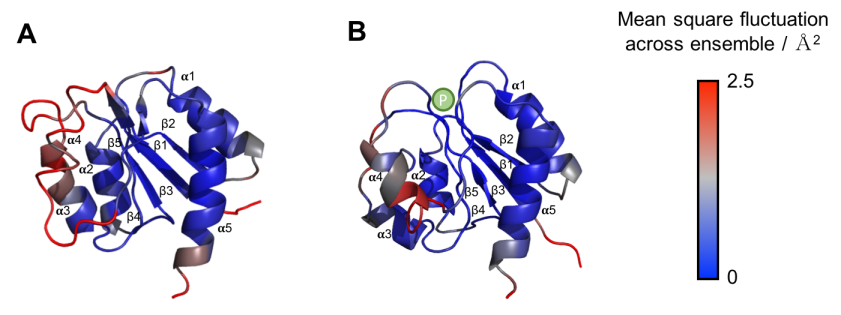
\includegraphics[width=\textwidth]{figures/ntrc/ntrc}

\caption{Ensembles of NtrC.
(A) The mean square fluctuation in the unperturbed ensemble is shown on the inactive structure (PDB ID 1DC7).
(B) The mean square fluctuation in the ensemble with additional constraints representing phosphorylation is shown in the active structure (PDB ID 1DC8).
Labels are taken from \cite{Volkman2001}.}

\label{fig:ntrc}
\end{figure}


\section{Discussion}

The allosteric prediction methods PARS, STRESS and AlloPred all use NMA to predict allosteric sites.
NMA is computationally-inexpensive and hence suitable for high-throughput, automated approaches.
However the assumption of harmonic fluctuations around an energetically-minimum structure often makes prediction of conformational changes difficult, particularly for transitions with a low degree of collectivity \cite{Yang2007}.
In addition, the choice of which normal modes to use is non-trivial.
Larger conformational changes are associated with low-frequency normal modes but higher-frequency modes are also required to take into account local effects.
The focus of NMA on changes in dynamics is also important - whilst NMA-based methods might be expected to reveal perturbations to vibrations in proteins there are a variety of other motions that contribute to allostery, such as local unfolding and rigid body movements \cite{Motlagh2014}.
By contrast, ExProSE generates native-like protein structures that can span large conformational changes.
The structure generation process is then perturbed to predict allosteric sites.
This has the potential to discover effects not revealed by NMA-based methods, whilst retaining the low computational cost and ease of use.
It also provides an ensemble of structures under the influence of the predicted modulator that can be used, for example, in flexible ligand docking.
Energy minimisation provides a way to improve the stereochemistry of generated structures for use in such approaches.

ExProSE requires two structures for each protein, whereas other methods only require one.
It also requires the structures to be different from each other in order to generate structures that span the conformational space.
This makes the method unsuitable for use on proteins where only one structure, or highly similar structures, are available.
However, many medically-important proteins have multiple structures available, including the examples used in this study.
In these cases, it makes sense to use the additional structural information.
The method also was successful at reproducing the allostery in CAP using only one structure as input.
For proteins with multiple different conformational states, more than two structures could be used as input to ExProSE to explore further regions of conformational space - the constraint combination procedure can be applied to an arbitrary number of structures.

For many ensemble generation methods, such as MD and tCONCOORD, the choice of parameters has a large effect on the structures produced.
The parameter in ExProSE with the largest effect is $W_{B}$ (see the experimental procedures), which affects the conformational spread of the ensemble.
Without any user input, the auto-parameterisation step of ExProSE selects a value that gives an ensemble well-spread over the conformational space between the two input structures.
Once $W_{B}$ has been selected automatically, an ensemble that spans the correct space is generally produced without any further choice of parameters.
This makes the method suitable for high-throughput structure generation across multiple proteins as the user does not need to make any parameter choices themselves.
The auto-parameterisation procedure can be adjusted to obtain the desired level of structural flexibility using the parameter $F$, which is intuitive in terms of the spread of structures over conformational space (see the experimental procedures).
This provides a way to generate an ensemble with more flexibility if the input structures are similar, as mentioned above.

In this study, LIGSITE\textsuperscript{\it cs} was used to predict pockets for ExProSE.
However, it is worth noting that any pocket prediction method that outputs pocket points is compatible with ExProSE without modification.
One of the challenges in allosteric site prediction is discovery of transient pockets - pockets that are only present in some structures of the ensemble.
There are currently no general methods that use transient pockets for allosteric site prediction \cite{Boehr2009}, though recent studies have used Markov state models on MD simulations to predict cryptic allosteric sites on multiple proteins \cite{Bowman2012, Bowman2015}.
These studies concluded that cryptic allosteric sites are more ubiquitous than previously thought.
ExProSE has the potential to identify transient pockets and predict their ability as allosteric sites.
For example, an ensemble could be clustered into a few representative structures and perturbation at sites on these structures could be used to predict transient allosteric pockets.

ExProSE builds on existing methods by using more structural information as input.
It is able to generate ensembles of protein structures that span relevant conformational changes in proteins.
This makes it an effective alternative to similar methods and to MD, which it is often not feasible to run on timescales long enough to explore large motions of interest without specialist approaches.
The perturbation procedure can be applied systematically to predict allosteric sites.
In a comparison of multiple allosteric site predictors, ExProSE showed performance similar to and complementary with existing methods.
Experimental results in the well-studied CAP were also reproduced by ExProSE.
The ability to generate ensembles of protein structures and investigate the response of an ensemble to perturbations should prove useful for both the exploration of individual proteins and the systematic study of the whole PDB.
Such methods are required to make sense of the increasing volume of structural data, and to understand the crucial importance of dynamics to protein function.


\chapter{CDK2}
\label{cha:cdk2}

This chapter describes computational and experimental work to test a potential allosteric site on cyclin-dependent kinase 2 (CDK2), a protein important in cell cycle regulation.
This allosteric site was predicted by ExProSE in Section~\ref{sec:exprose_results}.
A virtual screen of small molecules was carried out against the pocket.
Selected molecules were purchased and tested using two experimental assays to see if they could inhibit the interaction between CDK2 and cyclin A2.


\section{Materials and Methods}
\label{sec:cdk2_methods}


\subsection{Bioinformatics resources}

FTMap \cite{Kozakov2015}, the Fragment Hotspot Map \cite{Radoux2016}, ResiCon \cite{Dziubinski2016} and the DynOmics server \cite{Li2017} were run with default settings using the ANS-bound CDK2 structure (PDB ID 3PXF) as input.


\subsection{Virtual screening}

AutoDock Vina \cite{Trott2010} and DOCK \cite{Allen2015} were run in line with the respective documentation.
ChemMine \cite{Backman2011} clustering of structures used binning clustering at a similarity cutoff of 0.5.
The highest ranked by docking scores was retained in each case.

The ExProSE structures selected with an open pocket have the maximum sum of two distances across the opening of the pocket: the distance between atom OH on residue TYR180 and atom NH1 on ARG150, and the distance between atom OG on residue SER188 and atom O on THR165.
These structures are energy minimised as described in Section~\ref{sec:exprose_methods} to reduce any violations of stereochemistry.


\subsection{Reagents and compounds}

The buffers and media used for experimental work were as follows:
\begin{itemize}
\item Auto-induction media: 10 g/L tryptone, 5 g/L yeast extract, 5052, NPS, 1~M MgSO$_{4}$, Ampicillin.
\item Lysogeny broth: 10 g/L tryptone, 5 g/L yeast extract, 10 g/L NaCl.
\item Lysis buffer: 50 mM HEPES pH 7.0, 150 mM NaCl, 10 mM MgCl$_{2}$, 2 mM DTT, 1 mM EGTA, Triton.
\item Sodium phosphate pH 8 buffer: 100 mM sodium phosphate pH 8.0.
\item Tris pH 8 buffer: 100 mM Tris-HCl pH 8.0, 150 mM NaCl, 10 mM MgCl$_{2}$.
\item TBS-T buffer: 50 mM Tris-HCl pH 7.5, 150 mM NaCl, 0.1\% Tween 20.
\item Transfer buffer: 20\% methanol, 190 mM glycine, 25 mM Tris.
\end{itemize}


\subsection{Purification of cyclin A2}

The plasmid for cyclin A2 with either a His tag or GST tag (source - David J Mann unpublished) was transformed into \textit{E.\ coli} Tuner cells.
Various conditions for growth were tried in auto-induction media and lysogeny broth, similar to the approach in \cite{Wang2007}.
The final conditions used for His-tagged cyclin A2 were growth of cultures at 37$^{\circ}$C until optical density in auto-induction media, then incubation at 18$^{\circ}$C for 40 hours.
Cells were harvested by centrifugation (10 min at 5,000 rpm).
Harvested cells were resuspended in lysis buffer with 0.5 mg ml$^{-1}$ lysozyme.
After sonication and centrifugation (30 min at 16,000 rpm) the supernatant was incubated on Ni Sepharose Fast Flow beads in lysis buffer for 1 hour.
After washing the beads, cyclin A2 was eluted with 500 mM imidazole in lysis buffer, dialysed into lysis buffer and stored at -20$^{\circ}$C in 50\% glycerol.


\subsection{TR-FRET assay}

To label CDK2 with Cy5 dye, CDK2 (source - Gregory Craven unpublished, 10 mg/ml) in sodium phosphate pH 8 buffer was incubated overnight with Cy5 NHS ester dye in anhydrous DMF.
Excess dye was removed by gel filtration in sodium phosphate pH 8 buffer with the fractions containing CDK2 identified by fluorescent SDS-PAGE.

For the time-resolved F\"{o}rster resonance energy transfer (TR-FRET) CDK2 titration each well contained 20 \textmu L volume of 1 nM cyclin A2-His, 1 nM Eu-anti-His antibody and CDK2 at various concentrations in 50\% glycerol/50\% sodium phosphate pH 8 buffer.
A control with no CDK2 and 10 CDK2 concentrations were used - 1 \textmu M, 300 nM, 100 nM, 30 nM, 10 nM, 3 nM, 1 nM, 300 pM, 100 pM and 50 pM.
The plate was incubated for 1 hour and centrifuged at 800 rpm before being read.
20 recordings were made by the plate reader and the values averaged.


\subsection{Binding assay}

His-tagged cyclin A2 (75 nM) was incubated on Ni Sepharose Fast Flow beads in Tris pH 8 buffer with 12\% DMSO.
CDK2 (source - Gregory Craven unpublished) was added (8 nM) along with compounds in 5 concentrations: 0 M control, 8 \textmu M, 40 \textmu M, 200 \textmu M and 1 mM.
After incubation for 1 hour the beads were washed with Tris pH 8 buffer and heated in gel-loading dye at 100$^{\circ}$C for 10 minutes to release bound protein.
The proteins in the supernatant were separated by SDS-PAGE and transferred to a nitrocellulose membrane by electroblotting in transfer buffer for 1 hour at 100 V.
The membrane was incubated for 15 minutes in TBS-T buffer with 1.5\% skimmed milk powder.
The primary antibody, CDK2 rabbit polyclonal antibody was added and the membrane incubated overnight at 4$^{\circ}$C.
After washing with TBS-T buffer the secondary antibody was added and incubation for 1 hour carried out.
The membrane was washed with TBS-T buffer and imaged with chemiluminescence by adding ECL dye and using a 1 s exposure.


\section{Results}
\label{sec:cdk2_results}

Having predicted a new allosteric site on CDK2 using ExProSE, we wished to explore this pocket further computationally and test experimentally whether it was in fact an allosteric site.
Section~\ref{sec:exprose_results} and Figure~\ref{fig:cdk2_exprose} describe how ExProSE predicts the third predicted pocket, henceforth referred to as the pocket of interest, as being allosteric.
See Figure~\ref{fig:cdk2_intro} for the structural elements of CDK2.
These pockets are also shown in Figure~\ref{fig:cdk2_structure}A.
The pocket of interest is close to the region of cyclin binding, as shown in Figure~\ref{fig:cdk2_structure}B with the non-crystallised portion of cyclin A2 modelled with Phyre2 \cite{Kelley2015}.

This pocket is not open in the apo CDK2 structure (PDB ID 1HCL) or in the cyclin A2-bound structure (PDB ID 1FIN).
In the cyclin A2-bound structure there is in fact a protrusion instead of a pocket opening, suggesting that a small molecule would not be able to bind the pocket at the same time as cyclin A2 is bound to CDK2.
The pocket is shown in Figure~\ref{fig:cdk2_structure}C in various structures where it is open.
The residues that make up the pocket are shown in Figure~\ref{fig:cdk2_structure}D.
The pocket is open but small in the structure with two ANS molecules bound in the known allosteric site (PDB ID 3PXF), with a size of 45 \AA$^{3}$ predicted by LIGSITE\textsuperscript{\it cs}.
It is a similar shape in the structure with two ANS molecules and the ATP-binding site inhibitor staurosporine (PDB ID 4EZ7).
This structure also has the crystallisation artefact ethanediol crystallised at the pocket of interest, implying that binding there is possible.

A structure with ethanediol bound at the ANS site and an ATP-binding site inhibitor (PDB ID 4EZ3) appears to have the pocket slightly open.
This indicates that occupation of the ANS site and opening of the pocket of interest are linked, suggesting that if the pocket can be bound then the inactivating motions of the \textalpha C-helix will prevent cyclin binding and inactivate the protein.
The idea is that by stabilising the pocket of interest the inactive state is favoured and activation by cyclin A2 cannot occur.
The hope is that the pocket of interest can accommodate a small molecule ligand, and potentially that it can open further to present more binding interactions.

One risk of targeting this site is that the pocket is small, meaning a limited number of interactions can be made with a ligand.
The pocket is also only available in some states, meaning that there may be an energetic cost to stabilising it \cite{Oleinikovas2016}.
Off site binding may also be a problem - the ATP-binding site and ANS allosteric site present large pockets on CDK2 known to bind small molecules, and a molecule may bind there rather than at the pocket of interest.

CDK2 was examined with available bioinformatics resources.
FTMap \cite{Kozakov2015} and the Fragment Hotspot Map \cite{Radoux2016} sample the protein surface with molecular probes to find fragment binding hotspots.
FTMap \cite{Kozakov2015} does not predict the pocket of interest as a binding site.
The Fragment Hotspot Map \cite{Radoux2016} does not reveal the pocket of interest as a fragment binding site in the default map.
However adjusting the score cutoff does show there is some ability for fragment to bind to the pocket.

ResiCon calculates dynamic regions in proteins by considering contacts between residues \cite{Dziubinski2016}.
ResiCon was run on CDK2.
The pocket of interest seems to be on the edge of dynamic domains across a variety of given numbers of domain outputs, including the default result of two domains.
This indicates that the site could have the ability to cause structural rearrangement in distal parts of the protein by acting as a hinge that responds to ligand binding.
This is further evidenced by examining CDK2 using the DynOmics server \cite{Li2017}.
Residue that are close to the pocket of interest, such as ASP127 in the pocket, are predicted to be hinge residues that control the two slowest normal modes.

PDBFlex finds flexible regions in proteins based on all PDB depositions of the protein \cite{Hrabe2016}.
For CDK2 it indicates that the only real areas of variation in the structure is around the \textalpha C-helix and the T-loop, which is near the pocket of interest.


\begin{figure}
\centering

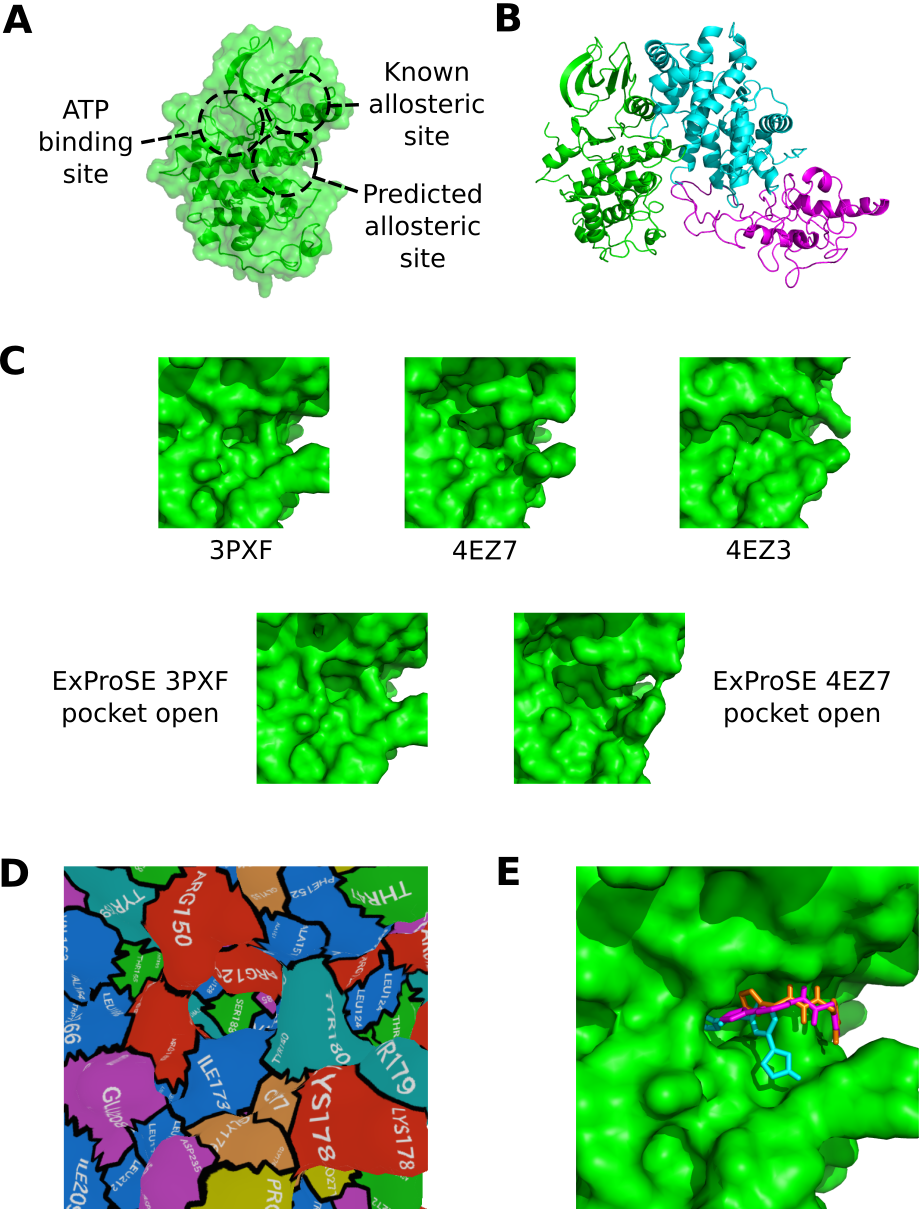
\includegraphics[width=0.95\textwidth]{figures/cdk2_structure/cdk2_structure}

\caption[Conformational variability and virtual screening of CDK2]
{Caption on following page.}

\label{fig:cdk2_structure}
\end{figure}

\begin{figure}

\contcaption{Structure, conformational variability and virtual screening of CDK2.
See also Figure~\ref{fig:cdk2_intro}.
(A) The structure of CDK2 (PDB ID 1HCL) with the ATP-binding site, the known allosteric site (ANS site) and the potential allosteric site (the pocket of interest) marked.
(B) The CDK2-cyclin A2 complex required for CDK2 activation.
The crystallised complex (PDB ID 1FIN) is shown with CDK2 in green and the crystallised portion of cyclin A2 in cyan.
The whole cyclin A2 sequence was modelled using Phyre2 \cite{Kelley2015} and aligned to the above complex and the ab initio modelled region (with no structural templates) is shown in magenta.
Part of this region potentially interacts with CDK2.
(C) The pocket of interest on CDK2 shown in various structures.
This is pocket 3 from Figure~\ref{fig:cdk2_exprose}.
The structures shown are three crystal structures with the PDB IDs given, and two structures with the pocket open generated using ExProSE from the structures indicated.
(D) Residues displayed around the pocket of interest using SurfStamp (\url{https://yamule.github.io/SurfStamp-public}). % http://process.sakura.ne.jp/surfstamp/viewer/test.cgi?pdbid=3PXF
The orientation is the same as in C and the ANS-bound structure (PDB ID 3PXF) is used.
(E) Example docking poses of screened compounds using AutoDock Vina on the structure with PDB ID 3PXF.
Shown are the lowest energy poses for compound A (magenta), B (cyan) and C (orange) from Table~\ref{tab:enamine_compounds}.}

\end{figure}


\subsection{Virtual screening}

A virtual screening approach was carried out to predict compounds that bind to the pocket of interest.
ZINC is a free database of commercially-available compounds for virtual screening \cite{Sterling2015}.
The ZINC12 LeadsNow subset contains over 3 million lead-like molecules in stock at chosen suppliers.
Lead-like molecules have a molecular weight between 250 and 350, an octanol-water partition coefficient not greater than 3.5 and no more than 7 rotatable bonds.
These criteria give smaller and less lipophilic molecules than those that would conventionally end up being drugs, i.e.\ those that fit Lipinski's rule of five \cite{Lipinski2001}.
This is because at the hit stage the priority is finding effective scaffolds with high affinity per atom (ligand efficiency).
Elaboration of the structure with further functional groups generally occurs later and would usually result in the addition of chemical groups, raising the molecular weight.

The LeadsNow subset is clustered as described at \url{http://zinc.docking.org} to get a representative subset of $\sim$250,000 compounds.
Each molecule has a Tanimoto coefficient, a similarity score that compares chemical fingerprints, of no more than 0.9 with any other molecule.
These compounds are docked using AutoDock Vina \cite{Trott2010} with standard settings to the pocket of interest in the ANS-bound structure (PDB ID 3PXF).
Examples of docking poses can be seen in Figure~\ref{fig:cdk2_structure}E.
The top 2,000 structures by affinity score from this screen were retained for further docking studies.
This was due to the computational cost of virtual screening - the score from AutoDock Vina on the ANS-bound structure was used to eliminate most compounds and the remaining compounds were taken forward for further studies.
The 2,000 retained molecules were docked using AutoDock Vina and DOCK \cite{Allen2015} onto four structures:
\begin{enumerate}
\item The ANS-bound structure, PDB ID 3PXF.
\item The ANS-bound structure with the ATP-binding site inhibitor staurosporine, PDB ID 4EZ7.
\item A structure selected from an ensemble of structures generated from (1) using ExProSE.
The structure selected is the one with the pocket of interest most open.
\item The same as (3) but the ensemble is generated using ExProSE from (2).
\end{enumerate}
The structure of the pocket of interest in each of these structures is shown in Figure~\ref{fig:cdk2_structure}C.
Docking to multiple structures means the compounds are scored in multiple conformations of the binding site, which is an approximation of ensemble docking.
This is important in general to take into account the flexibility of binding pockets, and especially important for this pocket as it is a flexible pocket not present in all structures.
Using two different docking algorithms, AutoDock Vina and DOCK, provides two different scores for each structure and goes some way to reducing the inaccuracies of virtual screening.
Compounds were in general better scored for structures (3) and (4), those with the pocket of interest open.
This is to be expected as a larger pocket presents more opportunities for interactions with the ligand.


\subsection{Compound selection}

Compounds were ranked by the average of the 8 scores from the above docking (4 structures, 2 docking methods).
In addition to the lead-like properties described previously, compounds were further filtered to remove compounds that would potentially give erroneous assay results.
Compounds violating various criteria set out by the SwissADME server for assessing medicinal chemistry friendliness \cite{Daina2017}, such as properties of pan-assay interference compounds \cite{Baell2014}, were removed.
Compounds marked as not having benign chemical functionality in ZINC12 were also removed.
Although compounds were clustered by ZINC12 to remove similar compounds, some compounds were relatively similar to each other on visual inspection.
Compounds were hence removed by similarity in ChemMine \cite{Backman2011}.
The top 20 ranked compounds remaining that were available from Enamine (\url{http://www.enamine.net}) were purchased and taken forward for experimental testing.
Docking scores and compound IDs are shown in Table~\ref{tab:enamine_compounds}.
The structures of the compounds are shown in Figure~\ref{fig:compound_structures}.
A search of these structures in the PDB indicates that none are currently ligands in the PDB.
None appear in the ChEMBL database of bioactive drug-like small molecules \cite{Gaulton2017}.


\begin{sidewaystable}
\centering

\begin{footnotesize}
% Table generated by Excel2LaTeX from sheet 'compounds'
\begin{tabular}{ p{2cm} l l p{2.5cm} l l l l l l l l }
\hline
                             &                    &                     &                                                   & \multicolumn{4}{c}{\textbf{AutoDock Vina best energy}} & \multicolumn{4}{c}{\textbf{DOCK best grid score}} \\
                             &                    &                     &                                                   & \multicolumn{4}{c}{\textbf{/ kcal mol$^{-1}$}}         & \multicolumn{4}{c}{}                              \\
\textbf{Compound\newline ID} & \textbf{ZINC12 ID} & \textbf{Enamine ID} & \textbf{Molecular\newline weight\newline (g/mol)} & \textbf{A} & \textbf{B} & \textbf{C} & \textbf{D}      & \textbf{A} & \textbf{B} & \textbf{C} & \textbf{D} \\
\hline
A & ZINC06731189 & Z28083007   & 279.3 & -7.1 & -8.1 & -7.6 & -7.4 & -37.3 & -40.0 & -40.8 & -35.1 \\
B & ZINC29799246 & Z2241108787 & 281.3 & -7.4 & -7.9 & -7.9 & -7.7 & -31.2 & -38.9 & -39.7 & -32.4 \\
C & ZINC58182552 & Z953947716  & 273.3 & -7.2 & -7.4 & -7.8 & -7.4 & -32.8 & -39.3 & -41.5 & -36.0 \\
D & ZINC03275010 & Z56813876   & 280.3 & -7.3 & -7.3 & -7.3 & -7.7 & -36.5 & -39.2 & -40.6 & -36.3 \\
E & ZINC25129280 & Z125831222  & 281.3 & -7.3 & -7.8 & -7.1 & -7.5 & -32.8 & -41.2 & -39.9 & -38.8 \\
F & ZINC97022380 & Z1537396696 & 280.3 & -7.7 & -7.6 & -7.4 & -7.8 & -35.0 & -37.0 & -38.2 & -32.6 \\
G & ZINC84057181 & Z1367181624 & 280.3 & -7.2 & -7.8 & -7.9 & -7.4 & -30.9 & -37.8 & -35.5 & -37.1 \\
H & ZINC30691564 & Z383528790  & 281.3 & -7.2 & -7.2 & -7.8 & -7.8 & -35.3 & -35.3 & -41.6 & -33.8 \\
I & ZINC36390489 & Z381531134  & 279.3 & -7.6 & -7.3 & -7.5 & -7.5 & -31.2 & -39.3 & -37.5 & -34.7 \\
J & ZINC89878745 & Z1159552572 & 279.3 & -7.0 & -8.0 & -8.3 & -7.2 & -37.3 & -38.3 & -38.9 & -32.5 \\
K & ZINC12812500 & Z220404550  & 279.3 & -7.0 & -7.9 & -7.5 & -7.7 & -31.8 & -38.1 & -39.0 & -34.6 \\
L & ZINC75147268 & Z1262428103 & 281.3 & -7.3 & -7.8 & -7.8 & -7.5 & -28.8 & -36.0 & -37.6 & -34.4 \\
M & ZINC71914433 & Z1232176487 & 274.3 & -7.0 & -7.4 & -7.4 & -7.5 & -36.2 & -37.6 & -40.2 & -35.7 \\
N & ZINC72288573 & Z1229931451 & 268.3 & -7.7 & -7.8 & -7.9 & -7.4 & -29.4 & -36.2 & -33.3 & -34.1 \\
O & ZINC69453509 & Z1030096350 & 287.4 & -7.2 & -7.6 & -7.1 & -7.7 & -33.9 & -40.5 & -33.1 & -35.8 \\
P & ZINC79097391 & Z1408168262 & 281.3 & -7.0 & -7.6 & -7.6 & -7.3 & -33.7 & -38.5 & -37.5 & -33.8 \\
Q & ZINC16497227 & Z66926805   & 280.3 & -6.9 & -7.4 & -7.8 & -7.9 & -29.2 & -38.8 & -40.0 & -33.5 \\
R & ZINC23143433 & Z352550190  & 271.3 & -7.5 & -7.3 & -6.9 & -7.1 & -32.5 & -39.6 & -38.4 & -36.2 \\
S & ZINC89858262 & Z1162482939 & 273.3 & -7.2 & -7.3 & -8.3 & -7.4 & -23.9 & -35.1 & -39.6 & -36.2 \\
T & ZINC69369685 & Z1097406485 & 272.3 & -7.2 & -7.1 & -7.0 & -7.1 & -37.0 & -40.6 & -43.1 & -35.6 \\
\hline
\multicolumn{3}{r}{\textbf{Mean values}} & 278.3 & -7.3 & -7.6 & -7.6 & -7.5 & -32.8 & -38.4 & -38.8 & -35.0 \\
\hline
\end{tabular}
\end{footnotesize}

\caption[Selected compounds to screen experimentally against a potential allosteric site on CDK2]
{Selected compounds to screen experimentally against a potential allosteric site on CDK2.
ZINC12 ID is the ID in the ZINC12 database (\url{http://zinc.docking.org}).
Enamine ID is the ID at Enamine Ltd (\url{http://www.enamine.net}).
The AutoDock Vina best energy and DOCK best grid score are shown for each ligand docked to four structures:
(A) PDB ID 3PXF,
(B) PDB ID 4EZ7,
(C) ExProSE pocket open structure from 3PXF,
(D) ExProSE pocket open structure from 4EZ7.
See the main text for more information on these structures.
The mean values across the 20 compounds are also shown.}

\label{tab:enamine_compounds}
\end{sidewaystable}


\begin{figure}
\centering

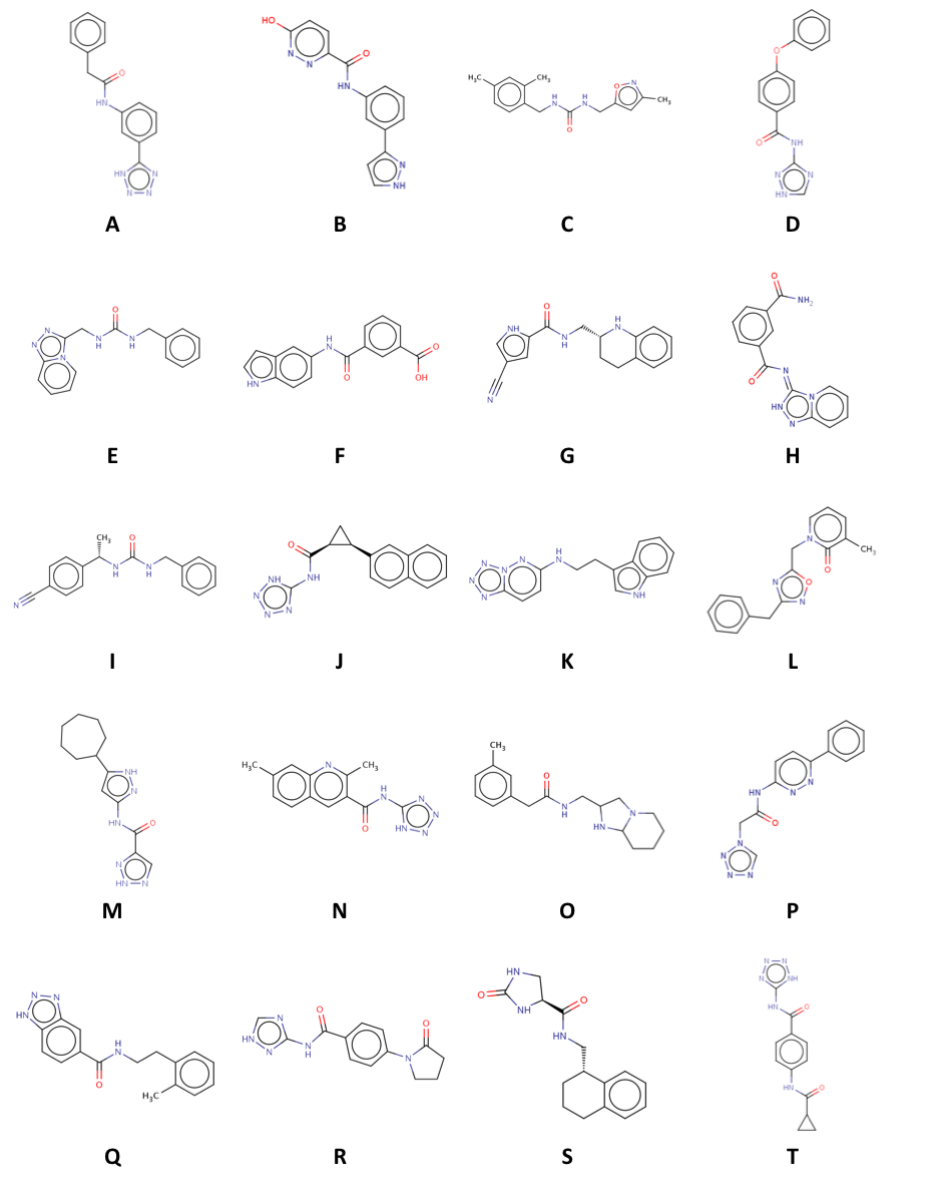
\includegraphics[width=0.9\textwidth]{figures/compound_structures/compound_structures}

\caption[Chemical structures of selected compounds to screen experimentally against a potential allosteric site on CDK2]
{Chemical structures of selected compounds to screen experimentally against a potential allosteric site on CDK2.
The compounds are labelled as in Table~\ref{tab:enamine_compounds}.
Images generated using \url{http://cdb.ics.uci.edu/cgibin/Smi2DepictWeb.py}.}

\label{fig:compound_structures}
\end{figure}


\subsection{Experimental aims}

The main aim of the experimental work was to screen the purchased compounds using the TR-FRET assay and a binding assay to see if the compounds could inhibit the CDK2-cyclin A2 interaction.
This required cyclin A2 to be purified.


\subsection{Purification of cyclin A2}

For optimal TR-FRET signal (see below) it is be beneficial to have a single surface-exposed cysteine labelled with Cy5 dye.
Cyclin A2 has two surface-exposed cysteine residues.
Hence, initial purification was attempted for cyclin A2 residues 169-432 with GST tag and the C327A mutation.
% The other surface-exposed is C193
The GST tag allowed selective separation of the protein during purification.
The His tag could not be used as this was going to be present on CDK2 to bind the donor fluorophore.
This purification resulted in low quantities of soluble protein ($<$ 1 mg from 4 L media) and purity was low, as shown in Figure~\ref{fig:purification}A.
Different purification strategies including varying the media, incubation temperature and incubation times were attempted but did not improve yield.

The difficulty of purifying this cyclin A2 mutant led us to try purification of cyclin A2 residues 169-432 with GST tag and no mutation.
This purified more readily than the mutant, as shown in Figure~\ref{fig:purification}B.
However the yield was still low (1 mg from 8 L media).
This could be because the cysteine mutation destabilises the protein, increasing its tendency to aggregate.
Concentration of the protein using spin filtration led to loss of the protein.
This, along with the low yield, suggests that cyclin A2-GST is unstable and has a tendency to aggregate and become insoluble \cite{Brown2015}.

Due to the difficulty of purifying cyclin A2-GST, a change was made to the experimental strategy.
The donor and acceptor fluorophores for the TR-FRET assay were switched so that the Eu anti-His antibody was targeted at cyclin A2 and CDK2 was conjugated with Cy5 dye - see later.
This required purification of cyclin A2 residues 169-432 with His tag.
This purification proved considerably more successful than cyclin A2-GST, with 10 mg produced from 4 L media - see Figure~\ref{fig:purification}C.
This indicates that the large GST tag may disrupt the stability or folding of cyclin A2, but the shorter His tag does not have the same effect.
Purified cyclin A2-His was taken forward for the TR-FRET assay.


\begin{figure}
\centering

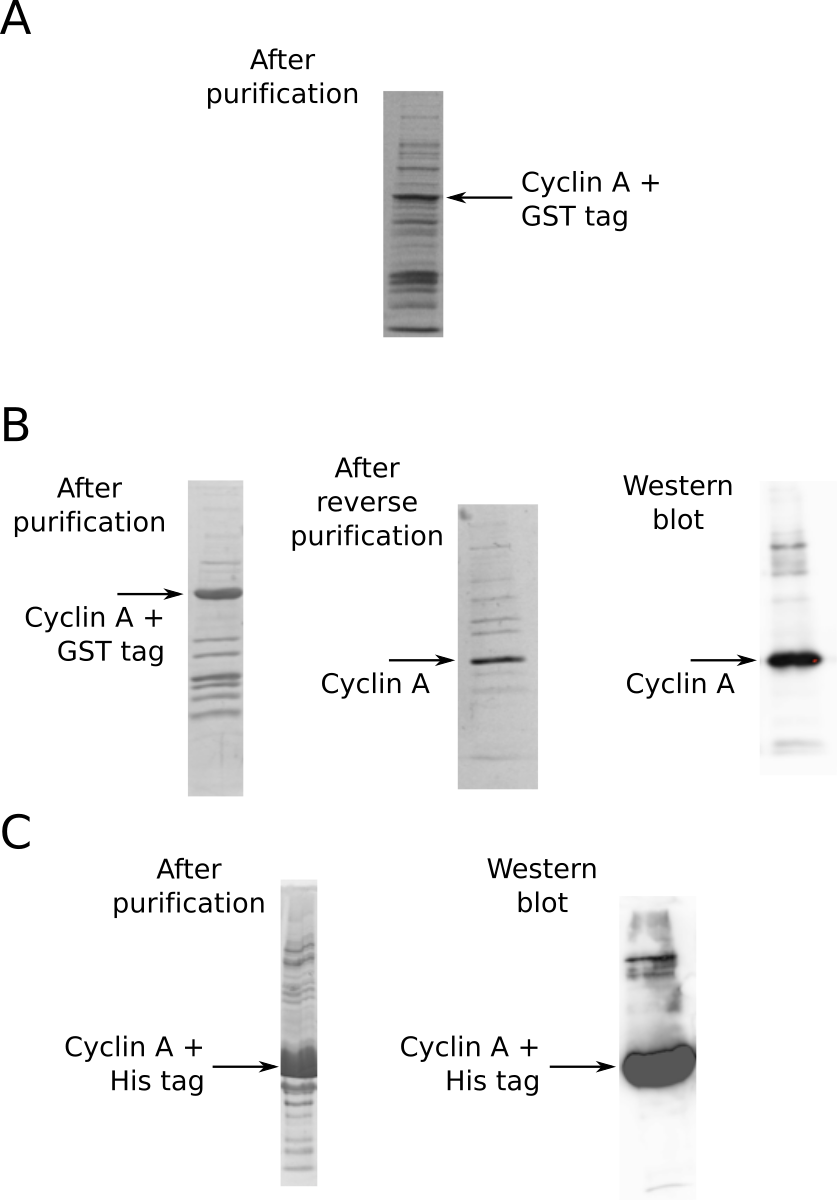
\includegraphics[width=0.6\textwidth]{figures/purification/purification}

\caption[SDS-PAGE results for purification of cyclin A2]
{SDS-PAGE results for purification of cyclin A2.
(A) Purification of cyclin A2 residues 169-432 with GST tag and the C327A mutation.
(B) Purification of cyclin A2 residues 169-432 with GST tag.
(C) Purification of cyclin A2 residues 169-432 with His tag.}

\label{fig:purification}
\end{figure}


\subsection{TR-FRET assay}

This popular assay for drug discovery research is the combination of time-resolved fluorometry with F\"{o}rster resonance energy transfer (FRET) \cite{Comley2006}.
Figure~\ref{fig:tr_fret}A and \ref{fig:tr_fret}B outline the principles of a TR-FRET assay.
FRET involves two fluorophores, a donor and an acceptor.
A time delay between excitation and detection means measurement occurs after the timescale of background fluorescence.
The long emission time of the donor fluorophore means a signal is obtained after the time delay.

CDK2 prepared previously in the lab was labelled with Cy5 dye.
The TR-FRET assay was tested using a titration of CDK2 with constant cyclin A2 and donor fluorophore.
An increase in signal with increasing CDK2 concentration would be expected.
Figure~\ref{fig:tr_fret}C shows the result of this titration.
Whilst there is a higher signal at higher CDK2 concentrations, this trend is also present for the control of cyclin A2-GST.
Cyclin A2-GST lacks the His tag required to bind to the donor fluorophore so should not lead to a TR-FRET signal.
This indicates that the increased signal with CDK2 concentration is likely due to excess, unbound Cy5 dye in the CDK2 solution.
Time constraints meant that a further gel filtration could not be carried out to remove this unbound dye.
The high background signal means the screen would not be effective at finding compounds that inhibit the cyclin A2-CDK2 interaction, so the compounds were not put through the TR-FRET screen.


\begin{figure}
\centering

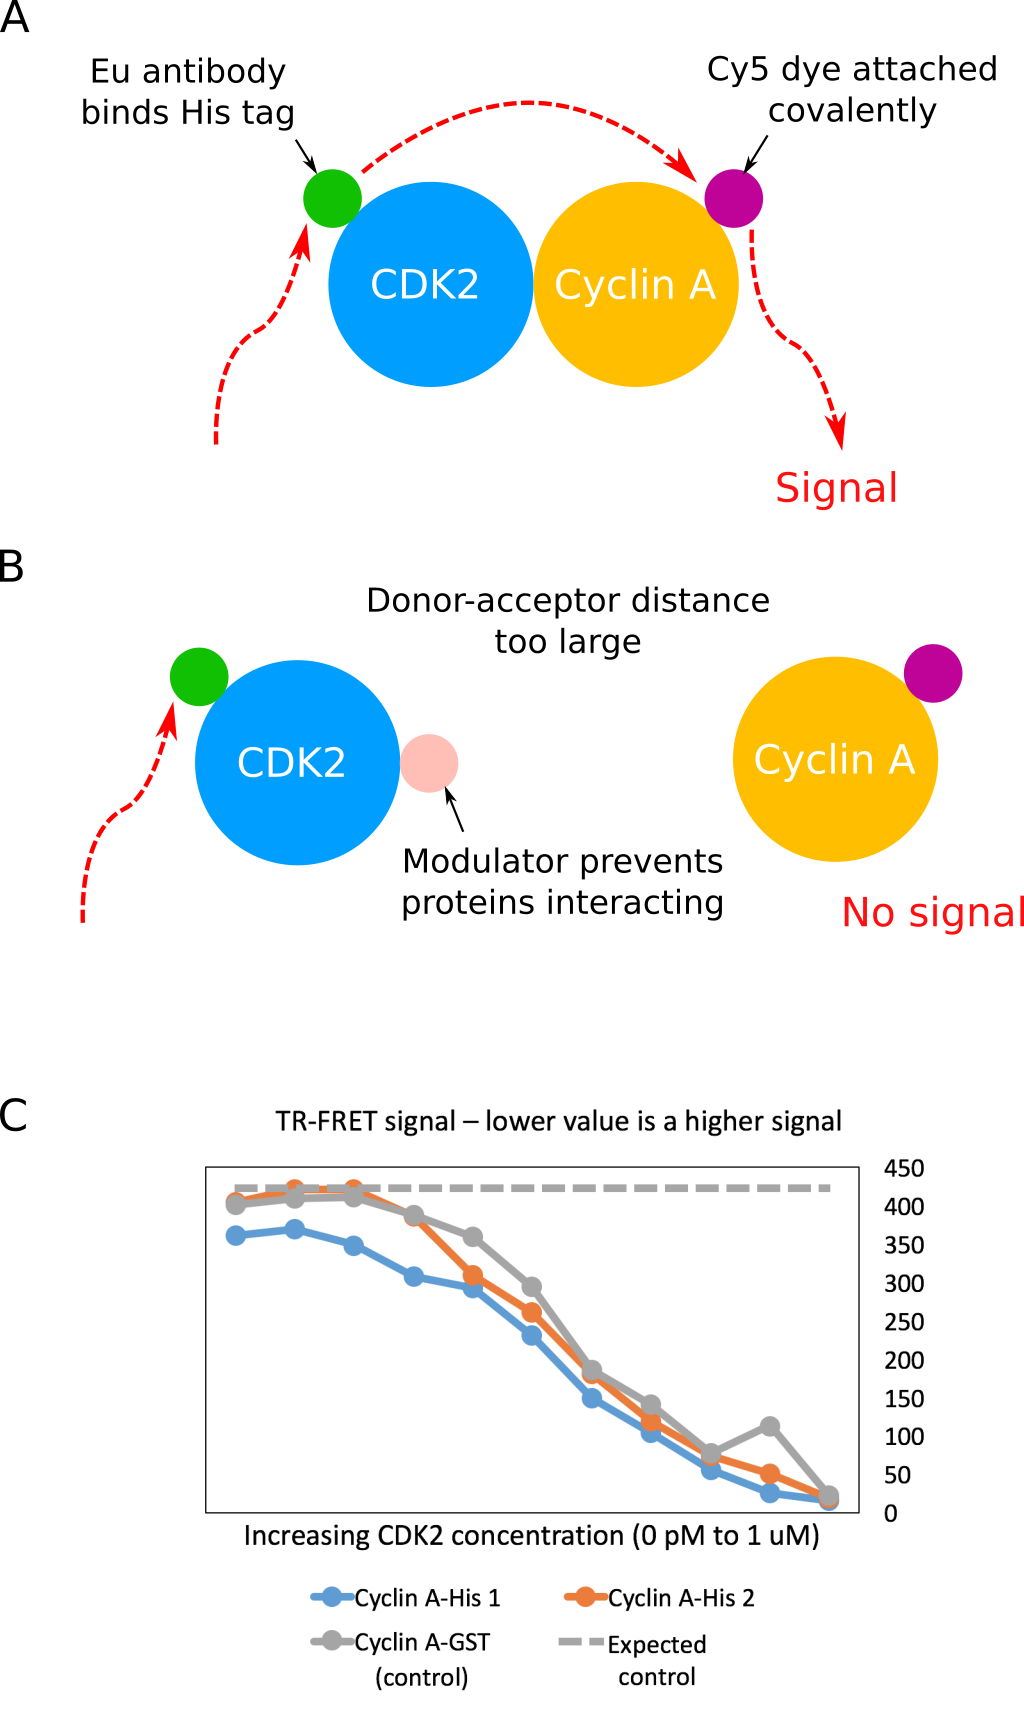
\includegraphics[width=0.7\textwidth]{figures/tr_fret/tr_fret}

\caption[TR-FRET assay principles and results]
{Caption on following page.}

\label{fig:tr_fret}
\end{figure}

\begin{figure}

\contcaption{(A) The principle of the TR-FRET assay used.
One protein in the binding pair is covalently-bound to Cy5 dye (the acceptor fluorophore).
The other protein is targeted with an antibody containing the lanthanide Eu (the donor fluorophore).
Light is shone at the excitation wavelength of the donor fluorophore.
This emits at the excitation wavelength of the acceptor fluorophore.
After a delay to allow background emission to recede, emission from the acceptor fluorophore is measured.
(B) If a modulator prevents the proteins interacting, emission from the donor to the acceptor fluorophore is not possible and there is no signal.
After difficulty purifying cyclin A2-GST, the strategy was switched so cyclin A2-His binds the Eu antibody and CDK2 is labelled with the dye.
(C) Results of a CDK2 titration TR-FRET assay.
The TR-FRET signal is shown for two repeats using cyclin A2-His, and for the control cyclin A2-GST which did not show the expected behaviour of a flat signal.}

\end{figure}


\subsection{Binding assay}

A binding assay was carried out to test whether the compounds could inhibit the CDK2-cyclin A2 interaction.
Cyclin A2-His and CDK2 were incubated with beads that selectively bind the His tag.
After washing the beads to remove unbound protein only cyclin A2 and proteins bound to it should remain.
In the absence of a binding inhibitor a signal for CDK2 would be expected in immunoblotting as CDK2 binds to cyclin A2.
This signal would be expected to disappear in the presence of a modulator that prevented the interaction.
This is only a semi-quantitative assay at best and TR-FRET would be much more informative.
However, it was carried out due to time constraints and the difficulties with obtaining results from TR-FRET.

The binding assay results can be seen in Figure~\ref{fig:binding_assay} for the 12 compounds it was carried out on.
A problem with the assay was binding of CDK2 to the beads despite the lack of a His tag on CDK2.
This gave a substantial background signal making a signal from the compounds hard to distinguish from the background.
However, some compounds do appear to remove the CDK2 signal at high concentrations.
Compound D at 200 \textmu M and 1 mM, and compound J at 1 mM, cause the CDK2 signal to decrease.
At these concentrations Compounds D and J had solubility issues in the assay.
As the expected background is high the solubility issues are likely the cause of the observed signal rather than genuine binding inhibition.


\begin{figure}
\centering

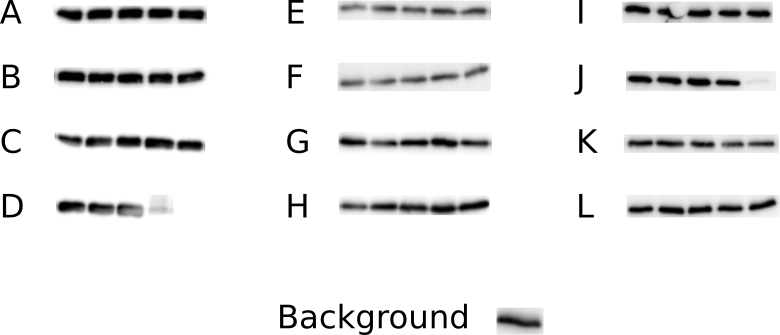
\includegraphics[width=0.7\textwidth]{figures/binding_assay/binding_assay}

\caption[Results of binding assay with selected compounds]
{Binding assay results for the 12 compounds tested.
The five bands represent increasing compound concentrations from left to right: 0 M control, 8 \textmu M, 40 \textmu M, 200 \textmu M and 1 mM.
The strength of the band represents the presence of CDK2.
The background signal, in the absence of cyclin A2, is also shown.
This shows non-specific binding of CDK2 to the beads and indicates that a signal in the assay would be hard to distinguish from the background.}

\label{fig:binding_assay}
\end{figure}


\section{Discussion}
\label{sec:cdk2_discussion}

The difficulty of purifying cyclin A2 is likely due to the propensity of the protein to aggregate.
This is probably due to large flexibility, a lack of stability in the absence of the binding partner and/or a partially folded state during expression \cite{Grigoroudis2015}.
This is exemplified by the fact that the crystal structure of the CDK2-cyclin A2 complex has only been found for part of the cyclin A2 structure \cite{Jeffrey1995}, as shown in Figure~\ref{fig:cdk2_structure}B.
In addition the full length of human cyclin A2 has not been crystallised in the absence of CDK2, with only the fragment corresponding to residues 171-432 in bovine cyclin A having a structure \cite{Brown1995}.
This is likely due to reasons related to the difficulties in purification.
The presence of the GST tag made the yield from cyclin A2 purification considerably lower than for the His tag.
This could be due to the large GST segment causing problems with folding leading to aggregation in the fusion protein.

Though time constraints meant that no more experiments could be carried out, there are a number of other tests that could be done to probe the allostery at the pocket of interest.
Primarily this would involve further work on the TR-FRET and binding assays to reduce background signal and allow the compounds to be screened.
Other tests that could be carried out include:

\begin{itemize}
\item Thermal shift assay: circular dichroism can be used to measure the unfolding of a protein by observing changes in plane-polarised light.
If a compound bound to CDK2 it may change the temperature at which the protein unfolds.
This assay is comparatively quick and easy but provides limited information.
\item Anti-proliferation assay: adding a compound to cancer cells should stop cell proliferation if the compound completely inhibits CDK2-cyclin A2 interaction.
However this assay does not indicate that the compound is specific to the CDK2-cyclin A2 interaction, as any effect that prevents proliferation will appear in the assay.
\item Mutagenesis: a mutation in the putative binding site of a compound will likely disrupt binding.
If inhibition occurs for the wild-type CDK2 but not for a mutant with a mutation, this gives evidence that the mutation site is the binding site or part of a crucial allosteric communication pathway.
This assumes that the mutation has no other effect on the structure such as destabilisation.
In addition, the effectiveness of mutagenesis studies to explore allostery has been questioned \cite{Tang2017}.
\item Cyclin E1: another cyclin that binds to CDK2 is cyclin E1.
Carrying out the above experiments with cyclin E1 rather than cyclin A2 would give an idea of the specificity of allosteric modulation of the interaction of CDK2 with cyclins.
Use of the different structures of cyclin A2 and cyclin E1 in complex with CDK2 may also help elucidate the allosteric mechanism \cite{Honda2005}.
\item Bovine cyclin A: bovine cyclin A purifies more readily than the human protein \cite{Brown2015} and this would provide an alternative source to the human protein.
\item Kinase assay: cyclin A2 is required for the activation, and hence kinase activity, of CDK2 \cite{Jeffrey1995}.
Assays that measure the kinase activity in the presence of the compounds indicate whether they are able to prevent CDK2 activation by cyclin A2.
\item Surface plasmon resonance (SPR): one binding partner is immobilised on a surface and the other partner is flowed across it.
The change in mass on the surface due to complex formation leads to a change in the refractive index of the solvent, which can be measured in real time.
SPR is a commonly-used tool to probe binding and would be suitable for the case of CDK2.
\item X-ray crystallography: hit compounds could be incubated with CDK2 and an attempt could be made at obtaining a crystal.
If successful this would indicate where the compound binds on CDK2 and show conformational changes due to binding.
It would also facilitate further computational studies on the new structure.

\end{itemize}

The difficulty of validating a predicted allosteric site experimentally acts as a deterrent to many groups.
However, the success of computational prediction methods is ultimately determined by whether they can make predictions that are validated experimentally.
In addition, iterative cycles of computational prediction and experimental validation can be used to develop and improve the computational approach, as has been seen recently for protein design applications \cite{Rocklin2017}.
The work in this chapter represents the first steps that would be taken on the path to experimental validation of a predicted site.
As more groups proceed from computational prediction to experimental validation \cite{Brecher2017} it is hoped that the path will become more established and systematic.


\chapter{Conclusion}
\label{cha:conclusion}

This thesis has explored the concept of allostery in proteins and developed methods for allosteric site prediction.
The background of allostery, a property of the protein structural ensemble, was introduced.
Two computational approaches were described.
AlloPred uses normal modes and machine learning to predict allosteric pockets on proteins.
ExProSE uses two structures of a protein to generate ensembles that span conformational space and can be perturbed to predict and explore allostery.
Allosteric prediction methods and virtual screening were used to predict modulators for a potential allosteric site on a protein kinase important for cell cycle control, CDK2.
These modulators were tested experimentally but the results were inconclusive.
Implications, discussion and further work for each of these approaches is described in the relevant chapters.

Themes of this work have included the benefits and drawbacks of NMA, MD and distance geometry methods; the separation of finding good binding sites in general with potential allosteric sites; the importance of experimental validation of computational predictions; and the difficulty of comparing allosteric prediction methods.
Ultimately, the variety of allosteric mechanisms and frameworks for studying allostery makes prediction challenging and indicates that more experimental and computational work is required in this important area.

For many years papers have pointed to the immense potential of allostery for both understanding and drugging proteins.
Yet they regularly contain the qualification that a unified framework of allostery remains `elusive', and approved allosteric drugs remain rare more than 50 years after the first descriptions of allostery.
In order to unlock the true potential of allostery, predictive methods need to be as established and robust as those in other areas of bioinformatics.
When allosteric prediction is as effective as prediction of secondary structure or disordered regions, the power of allostery will be truly revealed.
However the recent emergence of methods such as those presented here means the future of allosteric prediction looks bright.
In an analogous way to allostery itself, it is hoped that the effects of exploring allostery will propagate to all areas of structural biology.


\chapter{Appendices}
\label{cha:appendices}

\section{AlloPred documentation}

This section contains documentation for the AlloPred source code.
This documentation can be found along with the source code at \url{https://github.com/jgreener64/allopred}.


\subsection{Requirements}

\begin{itemize}
\item Python 2.7 with the NumPy and ProDy packages installed.
\item fpocket v2.0, which can be downloaded from \url{http://fpocket.sourceforge.net}. Follow the installation instructions to compile the executables.
\item SVM-light, which can be downloaded from \url{http://svmlight.joachims.org}. Follow the installation instructions to compile the executables.
\end{itemize}


\subsection{Usage}

Follow these steps to set up AlloPred - the shell commands are for bash:

\begin{enumerate}
\item Download the files and extract them as usual, or clone the repository.
\item The environmental variables \verb|$ALLOPRED_DIR| and \verb|$SVM_LIGHT_DIR| need to be set as the filepaths to the AlloPred directory and the SVM-light directory respectively:
\begin{lstlisting}[language=bash]
    export ALLOPRED_DIR=/path/to/allopred/
    export SVM_LIGHT_DIR=/path/to/svm_light/
\end{lstlisting}
Consider adding these lines to your profile so you don't have to run them every session.
\end{enumerate}

Follow these step to run AlloPred:

\begin{enumerate}
\item Obtain a PDB format file (\verb|in_file.pdb|), e.g.\ from the Protein Data Bank.

\item Create a one-line file (\verb|act_res.txt|) containing the active site residues of the protein. The format is \verb|10:A,11:B| for residue 10 on chain A and residue 11 on chain B. These can be found using resources such as the Catalytic Site Atlas. An example PDB file and active residue file can be found in the example directory of AlloPred.

\item Run fpocket v2.0 on the PDB file:
\begin{lstlisting}[language=bash]
    fpocket -f in_file.pdb
\end{lstlisting}
This assumes \verb|fpocket| is on the path. This produces the directory \verb|in_file_out|. AlloPred is optimised on the default fpocket parameters but you can change these in accordance with the fpocket documentation if you wish.

\item The following command, from the directory containing \verb|in_file.pdb| and \verb|in_file_out|, runs the AlloPred pipeline:
\begin{lstlisting}[language=bash]
    python $ALLOPRED_DIR/run_allopred.py in_file act_res.txt
\end{lstlisting}
The arguments are the input file prefix and the path to the active site residue file. Running the \verb|run_allopred.py| script with fewer than 2 arguments returns these instructions for the command.

\item The output files are:
    \begin{itemize}
    \item \verb|in_file.out|: the AlloPred output file containing the input parameters and the values for each pocket in order of AlloPred ranking.
    \item \verb|in_file.svm|: the SVM input file in the SVM-light format.
    \end{itemize}
\end{enumerate}


\subsection{Other files}

\begin{itemize}
\item \verb|dataset| contains information on the training and testing sets.
\item \verb|example| contains the inputs and outputs of an example run using the PDB entry with ID 1FX2.
\item \verb|svm_model.txt| is the optimised SVM built on the whole training set.
\end{itemize}


\section{ExProSE documentation}

This section contains documentation for the ExProSE source code.
This documentation can be found along with the source code at \url{https://github.com/jgreener64/ProteinEnsembles.jl}.
% Version info


\subsection{Summary}

Install using \verb|Pkg.add("ProteinEnsembles")| from within Julia v0.5. Run using

\begin{lstlisting}[language=bash]
    exprose --i1 input_1.pdb --d1 input_1.dssp \
        --i2 input_2.pdb --d2 input_2.dssp \
        -n 50 -o exprose_out
\end{lstlisting}

where \verb|exprose| is in the \verb|bin| directory.


\subsection{Installation}

Julia v0.5 is required and can be downloaded from \url{http://julialang.org/downloads}. Install ProteinEnsembles.jl by running \verb|Pkg.add("ProteinEnsembles")| from the Julia REPL. This will also automatically install a few other required Julia packages. If you want, the tests can be run using \verb|Pkg.test("ProteinEnsembles")|. If you wish to use the auto-parameterisation procedure (see below) you must also have TM-score installed.


\subsection{Requirements}

To use ProteinEnsembles.jl you will need the following:
\begin{itemize}
\item PDB files of the protein of interest. Two is best, but one may be used (see the paper). They must have polar hydrogens only added; this can be done using tools such as Chimera or pdbtools. The chain labelling and residue numbering must be consistent between the files as this is used to find common atoms. Alternative atom locations are discarded. PDB files must also be a single model and not have any inserted residues. HETATM records are discarded by default.
\item DSSP files corresponding to the PDB files above. These can be obtained using dssp.
\end{itemize}


\subsection{Usage}

These instructions are tailored towards Mac/Unix. However they could be modified to work on Windows.

Although organised as a Julia package, ProteinEnsembles.jl is primarily designed for use from the command line. The \verb|exprose| script in the \verb|bin| directory implements this. For example, to see the command line options run

\begin{lstlisting}[language=bash]
    ~/.julia/v0.5/ProteinEnsembles/bin/exprose -h
\end{lstlisting}

For easy access to the \verb|exprose| command you might like to add the following line to your profile:

\begin{lstlisting}[language=bash]
    export PATH=$PATH:~/.julia/v0.5/ProteinEnsembles/bin
\end{lstlisting}

Then, if all input files are in your current directory, run the program as follows:

\begin{lstlisting}[language=bash]
    # Generate an ensemble of 50 structures with an output directory exprose_out
    exprose --i1 input_1.pdb --d1 input_1.dssp --i2 input_2.pdb \
        --d2 input_2.dssp -n 50 -o exprose_out

    # Use a tolerance weighting of 0.5
    exprose --i1 input_1.pdb --d1 input_1.dssp --i2 input_2.pdb \
        --d2 input_2.dssp -n 50 -o exprose_out -w 0.5

    # Generate an ensemble from a single structure with a tolerance weighting of 1.0
    exprose --i1 input_1.pdb --d1 input_1.dssp -n 50 -o exprose_out -w 1.0
\end{lstlisting}

The method may also be run from within Julia. The below Julia script does the same thing as the first example above:

\begin{lstlisting}
    using ProteinEnsembles
    runpipeline(
        i1="input_1.pdb",
        d1="input_1.dssp",
        i2="input_2.pdb",
        d2="input_2.dssp",
        n_strucs=50,
        out_dir="exprose_out"
    )
\end{lstlisting}

Or, to split it up a little into the constituent functions:

\begin{lstlisting}
    using ProteinEnsembles
    constraints_com, constraints_one, constraints_two = interactions(
        "input_1.pdb",
        "input_1.dssp",
        "input_2.pdb",
        "input_2.dssp"
    )
    ensemble_com = generateensemble(constraints_com, 50)
    runanalysis("exprose_out", ensemble_com, constraints_one, constraints_two)
\end{lstlisting}


\subsubsection{Selecting parameters}

The auto-parameterisation procedure can select a more suitable tolerance weighting value (see the paper). TM-score must be installed to do this. For example:

\begin{lstlisting}[language=bash]
    exprose-param --i1 input_1.pdb --d1 input_1.dssp --i2 input_2.pdb \
        --d2 input_2.dssp -o exprose_param -t TMscore
\end{lstlisting}

runs the auto-parameterisation procedure with the \verb|-t| option specifying the command to run TM-score. The last line of the output gives a suggested tolerance weighting. This value is also written out to \verb|suggested.tsv|. Use this value in a normal \verb|exprose| run as above.


\subsubsection{Allosteric site prediction}

To predict allosteric sites you should run LIGSITE\textsuperscript{\it cs} on the \emph{second} input structure (the one you give as \verb|--i2|). You then need to run the \verb|cluster-ligsite| script in \verb|bin| to assign the points to pockets:

\begin{lstlisting}[language=bash]
    cluster-ligsite pocket_r.pdb pocket_all.pdb pocket_points.pdb
\end{lstlisting}

where \verb|pocket_r.pdb| and \verb|pocket_all.pdb| are in the LIGSITE\textsuperscript{\it cs} output. Then carry out an \verb|exprose| run with the \verb|pocket_points.pdb| file (\verb|-l|) and the number of pockets (e.g.\ top 4) to perturb at (\verb|-m|) as parameters:

\begin{lstlisting}[language=bash]
    exprose --i1 input_1.pdb --d1 input_1.dssp --i2 input_2.pdb \
        --d2 input_2.dssp -n 50 -o exprose_out -l pocket_points.pdb -m 4
\end{lstlisting}

A tolerance weighting from an auto-parameterisation run can also be used here. View the \verb|predictions.tsv| output file to get the order of allosteric pocket predictions. Note that other pocket prediction software can be used provided you can get the output into the same format as \verb|pocket_points.pdb|, i.e. pocket cavity points with the pocket number in the residue number column.


\subsubsection{Output}

The output directory contains the following:
\begin{itemize}
\item \verb|input_1.pdb| and \verb|input_2.pdb|: atoms used from the input structures are written back out and superimposed.
\item \verb|pdbs|: generated structures in PDB format. Superimposed to \verb|input_1.pdb| and \verb|input_2.pdb|.
\item \verb|pcs|: projections onto the principal components (PCs) from the principal component analysis of the generated structures. Contains files for generated (\verb|pcs.tsv|) and input structures (\verb|pcs_input_1.tsv| and \verb|pcs_input_2.tsv|) - line n corresponds to structure n and column c corresponds to PC c. Has graphs of these for the first few PCs (\verb|pc_x_y.png|). Also includes a list of PCs ordered by decreasing distance between the input structures (\verb|pcs_input_dist.tsv|) and the percentage variation explained by each PC (\verb|evals_spread.tsv|).
\item \verb|pymol|: PyMol scripts to view PCs on \verb|input_1.pdb|, e.g.\ run\newline \verb|pymol input_1.pdb pymol/view_pc_1.pml|.
\item \verb|rmsds_input_1.tsv| and \verb|rmsds_input_2.tsv|: RMSDs of generated structures to the input structures. Line n corresponds to structure n.
\item \verb|rmsfs.tsv| and \verb|rmsfs.png|: RMSFs of each residue over the ensemble of generated structures, and a plot of this. Line n corresponds to residue index n.
\item \verb|spe_scores.tsv|: SPE error scores of generated structures (see paper). Line n corresponds to structure n.
\end{itemize}

For allosteric site prediction there will be \verb|pdbs_mod_n| and \verb|mod_n| containing similar information for each perturbed ensemble, as well as the ratio of RMSF values to the unperturbed ensemble (\verb|rmsfs_ratio.tsv|). There will also be the order of allosteric predictions (\verb|predictions.tsv|) and the size of the perturbation on modulating each site (\verb|perturbations.tsv|), which is the RMSD between the centroid structure of the perturbed and unperturbed ensembles.

The default plot colours are blue for generated structures, red for input structure 1, green for input structure 2 and orange for perturbed ensemble structures.


\section{BioJulia Bio.Structure module}

Open source software packages to parse PDB files and manipulate protein structures exist in many programming languages.
There are a lack of such packages in the Julia language so a new module, Bio.Structure, was contributed to the BioJulia project (\url{http://biojulia.net}).
Features of the package include fast PDB parsing, easy access to structural elements, iteration over elements, selector functions, downloading of PDB files, writing PDB files and spatial functions such as distances and Ramachandran angles.
The structure of the type heirarchy is based on Biopython \cite{Cock2009} and is shown in Figure~\ref{fig:model_structure}.
Examples of basic use cases for Bio.Structure are shown in Figure~\ref{fig:biojulia_example}.


\begin{figure}
\centering

\includegraphics[width=0.9\textwidth]{figures/model_structure/model_structure}

\caption[Hierarchy of types in the BioJulia Bio.Structure module]
{Hierarchy of types in the BioJulia Bio.Structure module.
Types, analogous to classes in other languages, are shown in text.
\texttt{StructuralElement}, \texttt{AbstractResidue} and \texttt{AbstractAtom} are abstract types and may not themselves be instantiated.
Concrete (i.e.\ not abstract) types are shown in bold text.
Subtypes, analogous to subclasses, are indicated by red dotted lines.
A blue line indicates that an instance of the type contains a list of the indicated type.
For example, a \texttt{Chain} contains multiple \texttt{AbstractResidue}s.}

\label{fig:model_structure}
\end{figure}


\begin{figure}
\centering

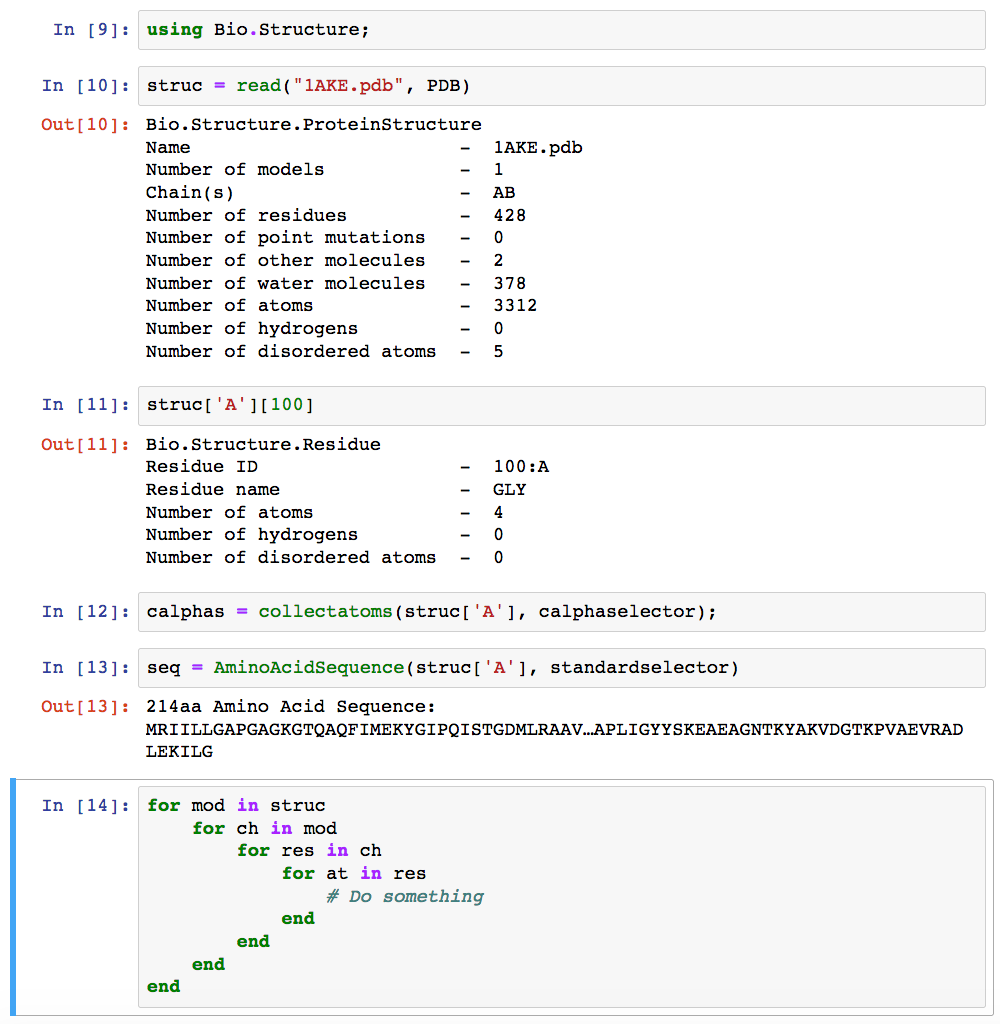
\includegraphics[width=0.9\textwidth]{figures/biojulia_example/biojulia_example}

\caption[Example functionality of the Bio.Structure module in the Jupyter Notebook]
{Example functionality of the Bio.Structure module.
The Jupyter Notebook and Julia v0.5.2 are used.
Cases shown are importing the module, reading in a PDB file, accessing residues by index, extracting C\textsuperscript{\textalpha} atoms, extracting the amino acid sequence and iterating over sub-elements.}
% cite Jupyter? Possibly http://ebooks.iospress.nl/publication/42900

\label{fig:biojulia_example}
\end{figure}


As part of the development of Bio.Structure information was collected on existing packages with similar functionality.
These comparisons are shown in Table~\ref{tab:package_comparison}.
The results of each package running various benchmarks are shown in Figure~\ref{fig:pdb_benchmarks}.
Bio.Structure is able to read in PDB file 1CRN in 1.4 ms (after just-in-time compilation) on average.
This is faster than any other package tested.


\begin{sidewaystable}
\centering

\begin{footnotesize}
\begin{tabular}{ l p{1.2cm} p{1.2cm} p{1.5cm} p{1.2cm} p{1.7cm} p{1.2cm} p{1.2cm} p{1.2cm} p{1.2cm} p{1.2cm} p{1.2cm} }
\hline
                      & BioJulia     & MIToS        & Biopython    & ProDy        & MDAnalysis   & Bio3D        & Rpdb         & BioPerl       & BioRuby      & Victor        & ESBTL        \\
\hline
Parse 1CRN / ms       & 1.4          & 2.4          & 9.1          & 2.2          & 6.4          & 31           & 19           & 63            & 25           & 10            & 6.8          \\
Parse 3JYV / s        & 0.49         & 0.74         & 1.0          & 0.28         & 0.80         & 14           & 2.2          & 3.8           & 0.98         & 7.7           & 0.95         \\
Parse 1HTQ / s        & 27           & 28           & 25           & 1.7          & 3.0          & 60           & 34           & 71            & 18           & 17            & -            \\
Count / ms            & 0.91         & 0.16         & 0.48         & 8.9          & 5.7          & 0.53         & 0.46         & 0.79          & 0.19         & -             & -            \\
Distance / ms         & 0.11         & 0.011        & 0.39         & 5.6          & 3.3          & 1.4          & 1.9          & 0.85          & 0.51         & -             & -            \\
Ramachandran / ms     & 13           & -            & 130          & 180          & 3500         & -            & -            & -             & -            & -             & -            \\
Language              & Julia        & Julia        & Python       & Python       & Python       & R            & R            & Perl          & Ruby         & C++           & C++          \\
Parses header         & $\times$     & $\times$     & $\checkmark$ & $\checkmark$ & $\times$     & $\checkmark$ & $\checkmark$ & $\times$      & $\checkmark$ & $\checkmark$  & $\times$     \\
Heirarchichal parsing & $\checkmark$ & $\times$     & $\checkmark$ & $\checkmark$ & $\checkmark$ & $\times$     & $\times$     & $\checkmark$  & $\checkmark$ & $\checkmark$  & $\checkmark$ \\
Supports disorder     & $\checkmark$ & $\times$     & $\checkmark$ & $\times$     & $\times$     & $\times$     & $\times$     & $\times$      & $\times$     & $\times$      & $\checkmark$ \\
Writes PDB files      & $\checkmark$ & $\checkmark$ & $\checkmark$ & $\checkmark$ & $\checkmark$ & $\checkmark$ & $\checkmark$ & $\checkmark$  & $\times$     & $\checkmark$  & $\checkmark$ \\
Superimposition       & $\times$     & $\checkmark$ & $\checkmark$ & $\checkmark$ & $\checkmark$ & $\checkmark$ & $\times$     & $\times$      & $\times$     & $\times$      & $\times$     \\
PCA                   & $\times$     & $\times$     & $\times$     & $\checkmark$ & $\checkmark$ & $\checkmark$ & $\times$     & $\times$      & $\times$     & $\times$      & $\times$     \\
Software license      & MIT          & MIT          & Biopython    & MIT          & GPLv2        & GPLv2        & GPL          & GPL/\newline Artistic  & Ruby         & GPLv3         & GPLv3        \\
\hline
\end{tabular}
\end{footnotesize}

\caption[Comparison of open source packages to read and manipulate PDB files in various programming languages]
{Comparison of open source packages to read and manipulate PDB files in various programming languages.
See Figure~\ref{fig:pdb_benchmarks} for descriptions and a visual representation of the benchmarks.}
% Do the methods need citation?

\label{tab:package_comparison}
\end{sidewaystable}


\begin{figure}
\centering

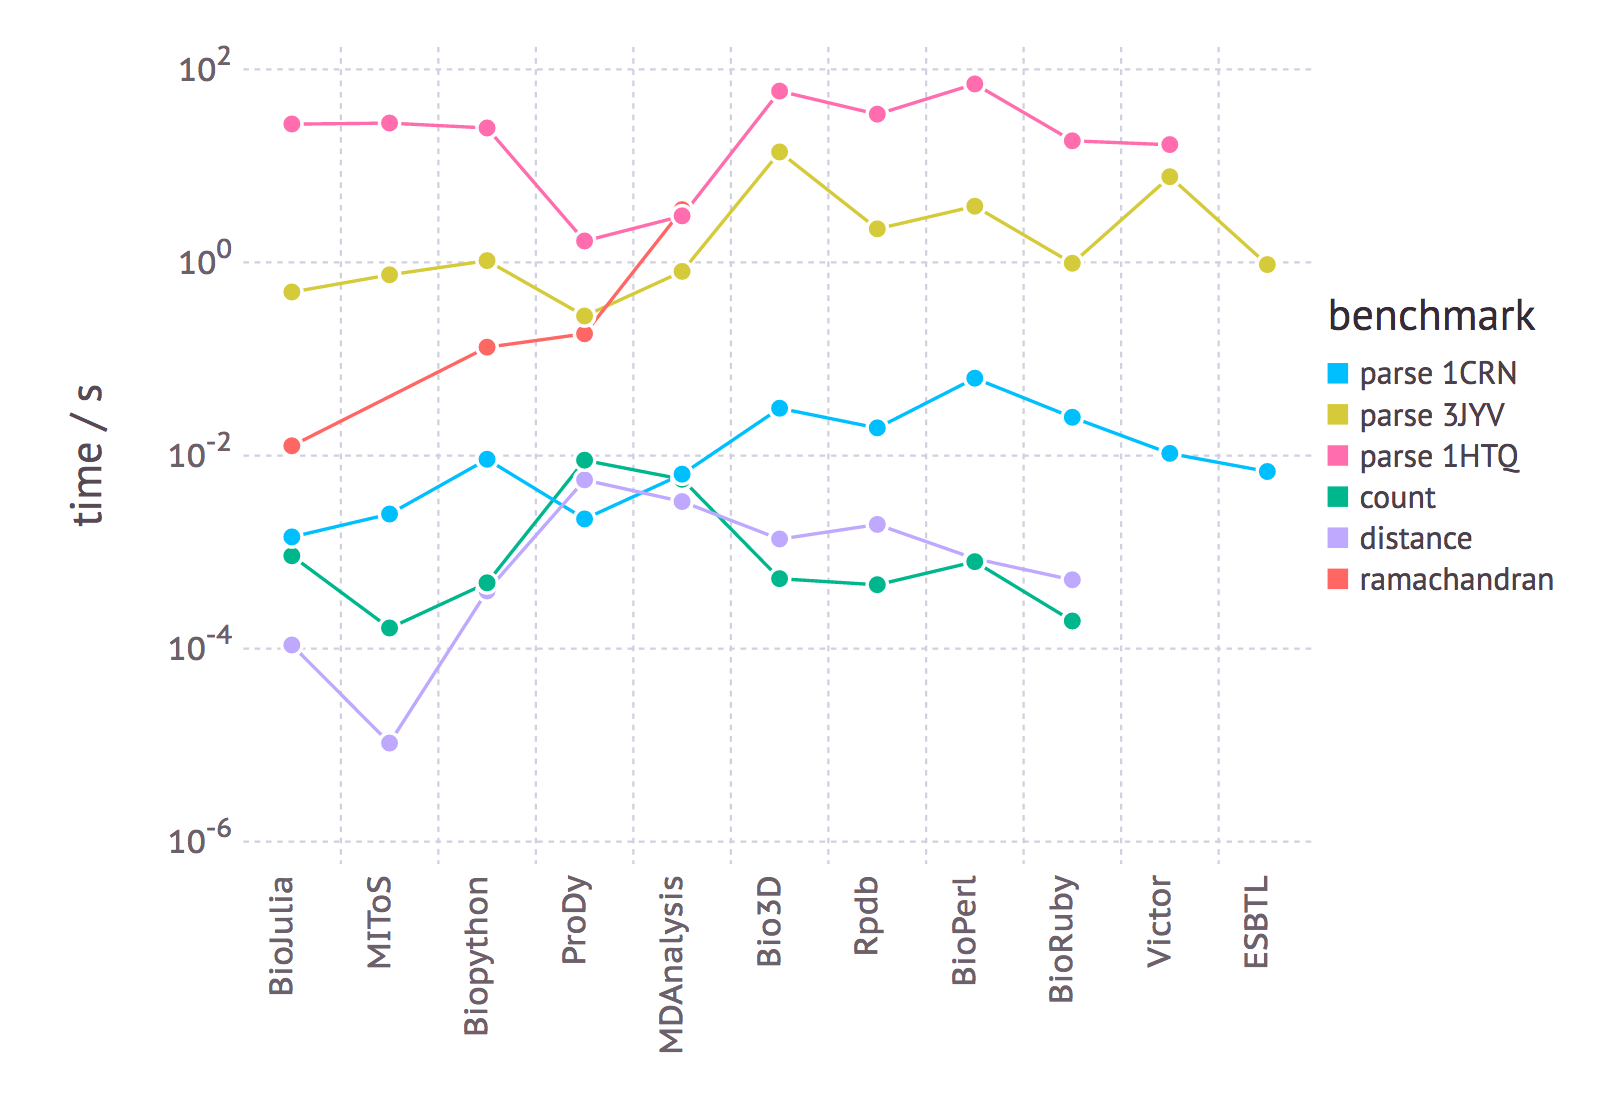
\includegraphics[width=0.9\textwidth]{figures/pdb_benchmarks/pdb_benchmarks}

\caption[Benchmarks on common tasks for open source packages to read and manipulate PDB files in various programming languages]
{Benchmarks on common tasks for open source packages to read and manipulate PDB files in various programming languages.
Benchmarks were carried out on a 3.1 GHz Intel Core i7 processor with 16 GB 1867 MHz DDR3 RAM.
The operating system was Mac OS X Yosemite 10.10.5.
Time is the elapsed time.
The mean over a number of runs is taken for each benchmark.
The three PDB files parsed are 1CRN (327 atoms), 3JYV (57,327 atoms) and 1HTQ (10 models of 97,872 atoms).
These are taken from the benchmarking in \cite{Gajda2013}.
`Count' is a count of the number of alanine residues in adenylate kinase (PDB ID 1AKE).
`Distance' is a calculation of the distance between residues 50 and 60 of chain A in adenylate kinase.
`Ramachandran' is a calculation of the Ramachandran \textphi /\textpsi\ angles in adenylate kinase.}

\label{fig:pdb_benchmarks}
\end{figure}


\singlespacing

\begin{small}
\renewcommand{\bibname}{References}
\bibliographystyle{unsrt}
\bibliography{library}
\end{small}

\end{document}
